% !TeX spellcheck = hu_HU
% !TeX encoding = UTF-8
% !TeX program = xelatex
% TODO Change language to en_GB (recommended) or en_US for English documents
\documentclass[11pt,a4paper,oneside]{report}             % Single-side
%\documentclass[11pt,a4paper,twoside,openright]{report}  % Duplex

% thanks to http://tex.stackexchange.com/a/47579/71109
\usepackage{ifxetex}
\usepackage{ifluatex}
\newif\ifxetexorluatex % a new conditional starts as false
\ifnum 0\ifxetex 1\fi\ifluatex 1\fi>0
   \xetexorluatextrue
\fi

\ifxetexorluatex
  \usepackage{fontspec}
\else
  \usepackage[T1]{fontenc}
  \usepackage[utf8]{inputenc}
  \usepackage[lighttt]{lmodern}
\fi

\usepackage[english,magyar]{babel} % Alapértelmezés szerint utoljára definiált nyelv lesz aktív, de később külön beállítjuk az aktív nyelvet.

%\usepackage{cmap}
\usepackage{amsfonts,amsmath,amssymb} % Mathematical symbols.
%\usepackage[ruled,boxed,resetcount,linesnumbered]{algorithm2e} % For pseudocodes. % beware: this is not compatible with LuaLaTeX, see http://tex.stackexchange.com/questions/34814/lualatex-and-algorithm2e
\usepackage{booktabs} % For publication quality tables for LaTeX
\usepackage{graphicx}

%\usepackage{fancyhdr}
%\usepackage{lastpage}

\usepackage{anysize}
%\usepackage{sectsty}
\usepackage{setspace} % For setting line spacing

\usepackage[unicode]{hyperref} % For hyperlinks in the generated document.
\usepackage[table,xcdraw]{xcolor}
\usepackage{listings} % For source code snippets.

\usepackage[amsmath,thmmarks]{ntheorem} % Theorem-like environments.

\usepackage[hang]{caption}

\singlespacing

\newcommand{\selecthungarian}{
	\selectlanguage{magyar}
	\setlength{\parindent}{2em}
	\setlength{\parskip}{0em}
	\frenchspacing
}

\newcommand{\selectenglish}{
	\selectlanguage{english}
	\setlength{\parindent}{0em}
	\setlength{\parskip}{0.5em}
	\nonfrenchspacing
	\renewcommand{\figureautorefname}{Figure}
	\renewcommand{\tableautorefname}{Table}
	\renewcommand{\partautorefname}{Part}
	\renewcommand{\chapterautorefname}{Chapter}
	\renewcommand{\sectionautorefname}{Section}
	\renewcommand{\subsectionautorefname}{Section}
	\renewcommand{\subsubsectionautorefname}{Section}
}

\usepackage[numbers]{natbib}
\usepackage{xspace}

\usepackage{enumerate}
\usepackage{enumitem}
\usepackage{multicol}
\usepackage{pythonhighlight}
\usepackage{minted}

\setsansfont{Calibri}
\setmonofont{Consolas}
\renewcommand{\theFancyVerbLine}{
	\sffamily\textcolor[rgb]{0.5,0.5,0.5}{\scriptsize\arabic{FancyVerbLine}}}

\usepackage{tabularx}
	\newcolumntype{L}{>{\raggedright\arraybackslash}X}
	
	
\usepackage{rotating}

\usepackage{csquotes}

\usepackage{algorithm}
\usepackage{algpseudocode}

%TODO Set the main variables
\newcommand{\vikszerzoVezeteknev}{Boér}
\newcommand{\vikszerzoKeresztnev}{Lehel}

\newcommand{\vikkonzulensAMegszolitas}{dr.~}
\newcommand{\vikkonzulensAVezeteknev}{Zainkó}
\newcommand{\vikkonzulensAKeresztnev}{Csaba}

\newcommand{\vikkonzulensBMegszolitas}{}
\newcommand{\vikkonzulensBVezeteknev}{}
\newcommand{\vikkonzulensBKeresztnev}{}

\newcommand{\vikkonzulensCMegszolitas}{}
\newcommand{\vikkonzulensCVezeteknev}{}
\newcommand{\vikkonzulensCKeresztnev}{}

\newcommand{\vikcim}{Biometrikus felhasználó azonosítás} % Cím
\newcommand{\viktanszek}{\bmemit} % Tanszék
\newcommand{\vikdoktipus}{\msc} % Dokumentum típusa (\bsc vagy \msc)
\newcommand{\vikmunkatipusat}{diplomatervet} % a "hallgató nyilatkozat" részhez: szakdolgozatot vagy diplomatervet

%--------------------------------------------------------------------------------------
% TDK-specifikus változók
%--------------------------------------------------------------------------------------
\newcommand{\tdkszerzoB}{Második Szerző} % Második szerző neve; hagyd üresen, ha egyedül írtad a TDK-t.
\newcommand{\tdkev}{2014} % A dolgozat írásának éve (pl. "2014") (Ez OTDK-nál eltérhet az aktuális évtől.)

% További adatok az OTDK címlaphoz (BME-s TDK-hoz nem kell kitölteni)
\newcommand{\tdkevfolyamA}{IV} % Első szerző évfolyama, római számmal (pl. IV).
\newcommand{\tdkevfolyamB}{III} % Második szerző évfolyama, római számmal (pl. III).
\newcommand{\tdkkonzulensbeosztasA}{egyetemi tanár} % Első konzulens beosztása (pl. egyetemi docens)
\newcommand{\tdkkonzulensbeosztasB}{doktorandusz} % Második konzulens beosztása (pl. egyetemi docens)

\newcommand{\szerzoMeta}{\vikszerzoVezeteknev{} \vikszerzoKeresztnev} % egy szerző esetén
%\newcommand{\szerzoMeta}{\vikszerzoVezeteknev{} \vikszerzoKeresztnev, \tdkszerzoB} % két szerző esetén

%TODO Language configuration -- choose one
% Beállítások magyar nyelvű dolgozathoz
%--------------------------------------------------------------------------------------
% Elnevezések
%--------------------------------------------------------------------------------------
\newcommand{\bme}{Budapesti Műszaki és Gazdaságtudományi Egyetem}
\newcommand{\vik}{Villamosmérnöki és Informatikai Kar}

\newcommand{\bmemit}{Méréstechnika és Információs Rendszerek Tanszék}

\newcommand{\keszitette}{Készítette}
\newcommand{\konzulens}{Konzulens}

\newcommand{\bsc}{Szakdolgozat}
\newcommand{\msc}{Diplomaterv}
\newcommand{\tdk}{TDK dolgozat}
\newcommand{\bsconlab}{BSc Önálló laboratórium}
\newcommand{\msconlabi}{MSc Önálló laboratórium 1.}
\newcommand{\msconlabii}{MSc Önálló laboratórium 2.}

\newcommand{\pelda}{Példa}
\newcommand{\definicio}{Definíció}
\newcommand{\tetel}{Tétel}

\newcommand{\bevezetes}{Bevezetés}
\newcommand{\koszonetnyilvanitas}{Köszönetnyilvánítás}
\newcommand{\fuggelek}{Függelék}

% Opcionálisan átnevezhető címek
%\addto\captionsmagyar{%
%\renewcommand{\listfigurename}{Saját ábrajegyzék cím}
%\renewcommand{\listtablename}{Saját táblázatjegyzék cím}
%\renewcommand{\bibname}{Saját irodalomjegyzék név}
%}

\newcommand{\szerzo}{\vikszerzoVezeteknev{} \vikszerzoKeresztnev}
\newcommand{\vikkonzulensA}{\vikkonzulensAMegszolitas\vikkonzulensAVezeteknev{} \vikkonzulensAKeresztnev}
\newcommand{\vikkonzulensB}{\vikkonzulensBMegszolitas\vikkonzulensBVezeteknev{} \vikkonzulensBKeresztnev}
\newcommand{\vikkonzulensC}{\vikkonzulensCMegszolitas\vikkonzulensCVezeteknev{} \vikkonzulensCKeresztnev}

\newcommand{\selectthesislanguage}{\selecthungarian}

\bibliographystyle{unsrt}

\def\lstlistingname{lista}

\newcommand{\appendixnumber}{6}  % a fofejezet-szamlalo az angol ABC 6. betuje (F) lesz

% Settings for English documents
%%--------------------------------------------------------------------------------------
% Elnevezések
%--------------------------------------------------------------------------------------
\newcommand{\bme}{Budapest University of Technology and Economics}
\newcommand{\vik}{Faculty of Electrical Engineering and Informatics}

\newcommand{\bmemit}{Department of Measurement and Information Systems}

\newcommand{\keszitette}{Author}
\newcommand{\konzulens}{Advisor}

\newcommand{\bsc}{Bachelor's Thesis}
\newcommand{\msc}{Master's Thesis}
\newcommand{\tdk}{Scientific Students' Association Report}
\newcommand{\bsconlab}{BSc Project Laboratory}
\newcommand{\msconlabi}{MSc Project Laboratory 1}
\newcommand{\msconlabii}{MSc Project Laboratory 2}

\newcommand{\pelda}{Example}
\newcommand{\definicio}{Definition}
\newcommand{\tetel}{Theorem}

\newcommand{\bevezetes}{Introduction}
\newcommand{\koszonetnyilvanitas}{Acknowledgements}
\newcommand{\fuggelek}{Appendix}

% Optional custom titles
%\addto\captionsenglish{%
%\renewcommand*{\listfigurename}{Your list of figures title}
%\renewcommand*{\listtablename}{Your list of tables title}
%\renewcommand*{\bibname}{Your bibliography title}
%}

\newcommand{\szerzo}{\vikszerzoKeresztnev{} \vikszerzoVezeteknev}
\newcommand{\vikkonzulensA}{\vikkonzulensAMegszolitas\vikkonzulensAKeresztnev{} \vikkonzulensAVezeteknev}
\newcommand{\vikkonzulensB}{\vikkonzulensBMegszolitas\vikkonzulensBKeresztnev{} \vikkonzulensBVezeteknev}
\newcommand{\vikkonzulensC}{\vikkonzulensCMegszolitas\vikkonzulensCKeresztnev{} \vikkonzulensCVezeteknev}

\newcommand{\selectthesislanguage}{\selectenglish}

\bibliographystyle{plainnat}

\newcommand{\ie}{i.e.\@\xspace}
\newcommand{\Ie}{I.e.\@\xspace}
\newcommand{\eg}{e.g.\@\xspace}
\newcommand{\Eg}{E.g.\@\xspace}
\newcommand{\etal}{et al.\@\xspace}
\newcommand{\etc}{etc.\@\xspace}
\newcommand{\vs}{vs.\@\xspace}
\newcommand{\viz}{viz.\@\xspace} % videlicet
\newcommand{\cf}{cf.\@\xspace} % confer
\newcommand{\Cf}{Cf.\@\xspace}
\newcommand{\wrt}{w.r.t.\@\xspace} % with respect to
\newcommand{\approximately}{approx.\@\xspace}

\newcommand{\appendixnumber}{1}  % a fofejezet-szamlalo az angol ABC 1. betuje (A) lesz


%--------------------------------------------------------------------------------------
% Page layout setup
%--------------------------------------------------------------------------------------
% we need to redefine the pagestyle plain
% another possibility is to use the body of this command without \fancypagestyle
% and use \pagestyle{fancy} but in that case the special pages
% (like the ToC, the References, and the Chapter pages)remain in plane style

\pagestyle{plain}
\marginsize{35mm}{25mm}{15mm}{15mm}

\setcounter{tocdepth}{3}
%\sectionfont{\large\upshape\bfseries}
\setcounter{secnumdepth}{3}

\sloppy % Margón túllógó sorok tiltása.
\widowpenalty=10000 \clubpenalty=10000 %A fattyú- és árvasorok elkerülése
\def\hyph{-\penalty0\hskip0pt\relax} % Kötőjeles szavak elválasztásának engedélyezése


%--------------------------------------------------------------------------------------
% Setup hyperref package
%--------------------------------------------------------------------------------------
\hypersetup{
    % bookmarks=true,            % show bookmarks bar?
    unicode=true,              % non-Latin characters in Acrobat's bookmarks
    pdftitle={\vikcim},        % title
    pdfauthor={\szerzoMeta},    % author
    pdfsubject={\vikdoktipus}, % subject of the document
    pdfcreator={\szerzoMeta},   % creator of the document
    pdfproducer={},    % producer of the document
    pdfkeywords={},    % list of keywords (separate then by comma)
    pdfnewwindow=true,         % links in new window
    colorlinks=true,           % false: boxed links; true: colored links
    linkcolor=black,           % color of internal links
    citecolor=black,           % color of links to bibliography
    filecolor=black,           % color of file links
    urlcolor=black             % color of external links
}


%--------------------------------------------------------------------------------------
% Set up listings
%--------------------------------------------------------------------------------------
\definecolor{lightgray}{rgb}{0.95,0.95,0.95}
\lstset{
	basicstyle=\scriptsize\ttfamily, % print whole listing small
	keywordstyle=\color{black}\bfseries, % bold black keywords
	identifierstyle=, % nothing happens
	% default behavior: comments in italic, to change use
	% commentstyle=\color{green}, % for e.g. green comments
	stringstyle=\scriptsize,
	showstringspaces=false, % no special string spaces
	aboveskip=3pt,
	belowskip=3pt,
	backgroundcolor=\color{lightgray},
	columns=flexible,
	keepspaces=true,
	escapeinside={(*@}{@*)},
	captionpos=b,
	breaklines=true,
	frame=single,
	float=!ht,
	tabsize=2,
	literate=*
		{á}{{\'a}}1	{é}{{\'e}}1	{í}{{\'i}}1	{ó}{{\'o}}1	{ö}{{\"o}}1	{ő}{{\H{o}}}1	{ú}{{\'u}}1	{ü}{{\"u}}1	{ű}{{\H{u}}}1
		{Á}{{\'A}}1	{É}{{\'E}}1	{Í}{{\'I}}1	{Ó}{{\'O}}1	{Ö}{{\"O}}1	{Ő}{{\H{O}}}1	{Ú}{{\'U}}1	{Ü}{{\"U}}1	{Ű}{{\H{U}}}1
}


%--------------------------------------------------------------------------------------
% Set up theorem-like environments
%--------------------------------------------------------------------------------------
% Using ntheorem package -- see http://www.math.washington.edu/tex-archive/macros/latex/contrib/ntheorem/ntheorem.pdf

\theoremstyle{plain}
\theoremseparator{.}
\newtheorem{example}{\pelda}

\theoremseparator{.}
%\theoremprework{\bigskip\hrule\medskip}
%\theorempostwork{\hrule\bigskip}
\theorembodyfont{\upshape}
\theoremsymbol{{\large \ensuremath{\centerdot}}}
\newtheorem{definition}{\definicio}

\theoremseparator{.}
%\theoremprework{\bigskip\hrule\medskip}
%\theorempostwork{\hrule\bigskip}
\newtheorem{theorem}{\tetel}


%--------------------------------------------------------------------------------------
% Some new commands and declarations
%--------------------------------------------------------------------------------------
\newcommand{\code}[1]{{\upshape\ttfamily\scriptsize\indent #1}}
\newcommand{\doi}[1]{DOI: \href{http://dx.doi.org/\detokenize{#1}}{\raggedright{\texttt{\detokenize{#1}}}}} % A hivatkozások közt így könnyebb DOI-t megadni.

\DeclareMathOperator*{\argmax}{arg\,max}
%\DeclareMathOperator*[1]{\floor}{arg\,max}
\DeclareMathOperator{\sign}{sgn}
\DeclareMathOperator{\rot}{rot}


%--------------------------------------------------------------------------------------
% Setup captions
%--------------------------------------------------------------------------------------
\captionsetup[figure]{
	width=.75\textwidth,
	aboveskip=10pt}

\renewcommand{\captionlabelfont}{\bf}
%\renewcommand{\captionfont}{\footnotesize\it}

%--------------------------------------------------------------------------------------
% Hyphenation exceptions
%--------------------------------------------------------------------------------------
\hyphenation{Shakes-peare Mar-seilles ár-víz-tű-rő tü-kör-fú-ró-gép}


\author{\vikszerzo}
\title{\viktitle}

%--------------------------------------------------------------------------------------
% Table of contents and the main text
%--------------------------------------------------------------------------------------
\begin{document}

\pagenumbering{gobble}

%TODO These includes define guidelines -- remove these
%~~~~~~~~~~~~~~~~~~~~~~~~~~~~~~~~~~~~~~~~~~~~~~~~~~~~~~~~~~~~~~~~~~~~~~~~~~~~~~~~~~~~~~
%\selecthungarian
%--------------------------------------------------------------------------------------
% Rovid formai es tartalmi tajekoztato
%--------------------------------------------------------------------------------------

\footnotesize
\begin{center}
\large
\textbf{\Large Általános információk, a diplomaterv szerkezete}\\
\end{center}

A diplomaterv szerkezete a BME Villamosmérnöki és Informatikai Karán:
\begin{enumerate}
\item	Diplomaterv feladatkiírás
\item	Címoldal
\item	Tartalomjegyzék
\item	A diplomatervező nyilatkozata az önálló munkáról és az elektronikus adatok kezeléséről
\item	Tartalmi összefoglaló magyarul és angolul
\item	Bevezetés: a feladat értelmezése, a tervezés célja, a feladat indokoltsága, a diplomaterv felépítésének rövid összefoglalása
\item	A feladatkiírás pontosítása és részletes elemzése
\item	Előzmények (irodalomkutatás, hasonló alkotások), az ezekből levonható következtetések
\item	A tervezés részletes leírása, a döntési lehetőségek értékelése és a választott megoldások indoklása
\item	A megtervezett műszaki alkotás értékelése, kritikai elemzése, továbbfejlesztési lehetőségek
\item	Esetleges köszönetnyilvánítások
\item	Részletes és pontos irodalomjegyzék
\item	Függelék(ek)
\end{enumerate}

Felhasználható a következő oldaltól kezdődő \LaTeX diplomatervsablon dokumentum tartalma. 

A diplomaterv szabványos méretű A4-es lapokra kerüljön. Az oldalak tükörmargóval készüljenek (mindenhol 2,5~cm, baloldalon 1~cm-es kötéssel). Az alapértelmezett betűkészlet a 12 pontos Times New Roman, másfeles sorközzel, de ettől kismértékben el lehet térni, ill. más betűtípus használata is megengedett.

Minden oldalon -- az első négy szerkezeti elem kivételével -- szerepelnie kell az oldalszámnak.

A fejezeteket decimális beosztással kell ellátni. Az ábrákat a megfelelő helyre be kell illeszteni, fejezetenként decimális számmal és kifejező címmel kell ellátni. A fejezeteket decimális aláosztással számozzuk, maximálisan 3 aláosztás mélységben (pl. 2.3.4.1.). Az ábrákat, táblázatokat és képleteket célszerű fejezetenként külön számozni (pl. 2.4. ábra, 4.2. táblázat vagy képletnél (3.2)). A fejezetcímeket igazítsuk balra, a normál szövegnél viszont használjunk sorkiegyenlítést. Az ábrákat, táblázatokat és a hozzájuk tartozó címet igazítsuk középre. A cím a jelölt rész alatt helyezkedjen el.

A képeket lehetőleg rajzoló programmal készítsék el, az egyenleteket egyenlet-szerkesztő segítségével írják le (A \LaTeX~ehhez kézenfekvő megoldásokat nyújt).

Az irodalomjegyzék szövegközi hivatkozása történhet sorszámozva (ez a preferált megoldás) vagy a Harvard-rendszerben (a szerző és az évszám megadásával). A teljes lista névsor szerinti sorrendben a szöveg végén szerepeljen (sorszámozott irodalmi hivatkozások esetén hivatkozási sorrendben). A szakirodalmi források címeit azonban mindig az eredeti nyelven kell megadni, esetleg zárójelben a fordítással. A listában szereplő valamennyi publikációra hivatkozni kell a szövegben (a \LaTeX-sablon a Bib\TeX~segítségével mindezt automatikusan kezeli). Minden publikáció a szerzők után a következő adatok szerepelnek: folyóirat cikkeknél a pontos cím, a folyóirat címe, évfolyam, szám, oldalszám tól-ig. A folyóiratok címét csak akkor rövidítsük, ha azok nagyon közismertek vagy nagyon hosszúak. Internetes hivatkozások megadásakor fontos, hogy az elérési út előtt megadjuk az oldal tulajdonosát és tartalmát (mivel a link egy idő után akár elérhetetlenné is válhat), valamint az elérés időpontját.

\vspace{5mm}
Fontos:
\begin{itemize}
	\item A szakdolgozatkészítő / diplomatervező nyilatkozata (a jelen sablonban szereplő szövegtartalommal) kötelező előírás, Karunkon ennek hiányában a szakdolgozat/diplomaterv nem bírálható és nem védhető!
	\item Mind a dolgozat, mind a melléklet maximálisan 15~MB méretű lehet!
\end{itemize}

\vspace{5mm}
\begin{center}
Jó munkát, sikeres szakdolgozatkészítést, ill. diplomatervezést kívánunk!
\end{center}

\normalsize
\selectthesislanguage

%%--------------------------------------------------------------------------------------
% Feladatkiiras (a tanszeken atveheto, kinyomtatott valtozat)
%--------------------------------------------------------------------------------------
\clearpage
\begin{center}
\large
\textbf{FELADATKIÍRÁS}\\
\end{center}

A feladatkiírást a tanszéki adminisztrációban lehet átvenni, és a leadott munkába eredeti, tanszéki pecséttel ellátott és a tanszékvezető által aláírt lapot kell belefűzni (ezen oldal \emph{helyett}, ez az oldal csak útmutatás). Az elektronikusan feltöltött dolgozatban már nem kell beleszerkeszteni ezt a feladatkiírást.


\selectthesislanguage

%TODO Titlepage -- choose one from below
%~~~~~~~~~~~~~~~~~~~~~~~~~~~~~~~~~~~~~~~~~~~~~~~~~~~~~~~~~~~~~~~~~~~~~~~~~~~~~~~~~~~~~~
\hypersetup{pageanchor=false}
%--------------------------------------------------------------------------------------
%	The title page
%--------------------------------------------------------------------------------------
\begin{titlepage}
\begin{center}

\includegraphics[width=60mm,keepaspectratio]{figures/bme_logo.pdf}\\
\vspace{0.3cm}
\textbf{\bme}\\
\textmd{\vik}\\
\textmd{\viktanszek}\\[5cm]

\vspace{0.4cm}
{\huge \bfseries \vikcim}\\[0.8cm]
\vspace{0.5cm}
\textsc{\Large \vikdoktipus}\\[4cm]

{
	\renewcommand{\arraystretch}{0.85}
	\begin{tabular}{cc}
	 \makebox[7cm]{\emph{\keszitette}} & \makebox[7cm]{\emph{\konzulens}} \\ \noalign{\smallskip}
	 \makebox[7cm]{\szerzo} & \makebox[7cm]{\vikkonzulensA} \\
	  & \makebox[7cm]{\vikkonzulensB} \\
	  & \makebox[7cm]{\vikkonzulensC} \\
	\end{tabular}
}

\vfill
{\large \today}
\end{center}
\end{titlepage}
\hypersetup{pageanchor=false}

		   % Szakdolgozat/Diplomaterv címlap
%%% TDK címlap
\begin{titlepage}
  \begin{center}  
  
\includegraphics[width=7cm]{./figures/bme_logo.pdf}
  \vspace{0.3cm}
  
  \bme \\
  \vik \\
  \viktanszek \\
  \vspace{5cm}
  
  \huge {\vikcim}
  \vspace{1.5cm}
  
  \large {\textbf{\tdk}}
  \vfill
    
  {\Large 
  	\keszitette: \\ \vspace{0.3cm}
  	\szerzo \\
	\tdkszerzoB \\
  	\vspace{1.5cm}
  	\konzulens: \\ \vspace{0.3cm}
  	\vikkonzulensA \\
  	\vikkonzulensB \\
  }
  
  \vspace{2cm}
  \large {\tdkev}
 \end{center}
\end{titlepage}
%% Címlap vége
	% TDK címlap
%%% OTDK külső címlap
\begin{titlepage}
  	$\;$ 
	\vspace{5cm}
	
	\begin{center}
	\Huge
	\textbf{TDK-dolgozat}\let\thefootnote\relax\footnote{A dolgozat bemutatását a XXXXXXXXX  ``Lorem ipsum dolor sit amet'' című program támogatta.}
	\end{center}
	
	\vspace{13cm}
	
	\Large
	\hspace{8cm} \szerzo
	
	\hspace{8cm} \tdkszerzoB
	
	\hspace{8cm} \tdkev.
\end{titlepage}

\newpage
\thispagestyle{empty}


%% OTDK belső címlap
\begin{titlepage}
  \begin{center}  
  
\includegraphics[width=7cm]{./figures/bme_logo.pdf}
  \vspace{0.3cm}
  
  \bme \\
  \vik \\
  \viktanszek \\
  \vspace{3.5cm}
  
  \huge {\vikcim}
  \vspace{1.5cm}
  
  \large {\textbf{\vikdoktipus}}
  \vfill
    
  {\Large 
  	{\large \keszitette:} \\ \vspace{0.2cm}
  	\szerzo \\ \tdkevfolyamA. évfolyam \\
	\vspace{0.5cm}
	\tdkszerzoB \\ \tdkevfolyamB. évfolyam \\
  	\vspace{1.5cm}
  	{\large \konzulens:} \\ \vspace{0.2cm}
  	\vikkonzulensA,\\ \tdkkonzulensbeosztasA \\
  	\vspace{0.5cm}
  	\vikkonzulensB,\\ \tdkkonzulensbeosztasB \\
  }
  
  \vspace{2cm}
  \large {\tdkev.}
  
 \end{center}
\end{titlepage}   % OTDK címlap


% Table of Contents
%~~~~~~~~~~~~~~~~~~~~~~~~~~~~~~~~~~~~~~~~~~~~~~~~~~~~~~~~~~~~~~~~~~~~~~~~~~~~~~~~~~~~~~
\tableofcontents\vfill


% Declaration and Abstract
%~~~~~~~~~~~~~~~~~~~~~~~~~~~~~~~~~~~~~~~~~~~~~~~~~~~~~~~~~~~~~~~~~~~~~~~~~~~~~~~~~~~~~~
\selectlanguage{magyar}
\pagenumbering{gobble}
%--------------------------------------------------------------------------------------
% Nyilatkozat
%--------------------------------------------------------------------------------------
\begin{center}
\large
\textbf{HALLGATÓI NYILATKOZAT}\\
\end{center}

Alulírott \emph{\vikszerzoVezeteknev{} \vikszerzoKeresztnev}, szigorló hallgató kijelentem, hogy ezt a \vikmunkatipusat{} meg nem engedett segítség nélkül, saját magam készítettem, csak a megadott forrásokat (szakirodalom, eszközök stb.) használtam fel. Minden olyan részt, melyet szó szerint, vagy azonos értelemben, de átfogalmazva más forrásból átvettem, egyértelműen, a forrás megadásával megjelöltem.

Hozzájárulok, hogy a jelen munkám alapadatait (szerző(k), cím, angol és magyar nyelvű tartalmi kivonat, készítés éve, konzulens(ek) neve) a BME VIK nyilvánosan hozzáférhető elektronikus formában, a munka teljes szövegét pedig az egyetem belső hálózatán keresztül (vagy autentikált felhasználók számára) közzétegye. Kijelentem, hogy a benyújtott munka és annak elektronikus verziója megegyezik. Dékáni engedéllyel titkosított diplomatervek esetén a dolgozat szövege csak 3 év eltelte után válik hozzáférhetővé.

\begin{flushleft}
\vspace*{1cm}
Budapest, \today
\end{flushleft}

\begin{flushright}
 \vspace*{1cm}
 \makebox[7cm]{\rule{6cm}{.4pt}}\\
 \makebox[7cm]{\emph{\vikszerzoVezeteknev{} \vikszerzoKeresztnev}}\\
 \makebox[7cm]{hallgató}
\end{flushright}
\thispagestyle{empty}

\vfill
\clearpage
\thispagestyle{empty} % an empty page

\selectthesislanguage
 %TODO Hallgatói nyilatkozat -- TDK és OTDK esetén törlendő!
\pagenumbering{roman}
\setcounter{page}{1}

\selecthungarian

%----------------------------------------------------------------------------
% Abstract in Hungarian
%----------------------------------------------------------------------------
\chapter*{Kivonat}\addcontentsline{toc}{chapter}{Kivonat}

A biometrikus azonosításra használható modern, neurális hálózat alapú beszélőfelismerés jelenleg széles körben kutatott, gyorsan fejlődő terület. Jelenleg nincs átfogó rendszerezés, összehasonlítás a rendszerek között és ingyenesen elérhető beszélőfelismerő alkalmazás sem különböző modellek teljesítményének összeméréshez.
\newline
\newline
Dolgozatomban bemutatom a korai beszélőfelismerő rendszereket, a mai modern neurális hálózat alapú megközelítéseket és az ingyenesen elérhető beszédadatbázisokat. Ismertetem a metatanítás fogalmát a hozzá kapcsolódó optimizációs technikákkal. Részletesen bemutatok két beszélőfelismerő modellt; egy módosított WaveNet architektúrát és egy sziámi konvolúciós hálózatot, amelyeken méréseket is végzek. Végül leírom az általam készített Android alapú beszélőfelismerő alkalmazás implementációs részleteit, optimizálását és a felhasználási lehetőségeit.


\vfill
\selectenglish


%----------------------------------------------------------------------------
% Abstract in English
%----------------------------------------------------------------------------
\chapter*{Abstract}\addcontentsline{toc}{chapter}{Abstract}

Modern neural network-based speech recognition for biometric identification is a widely researched, rapidly evolving field. There is currently no comprehensive systematisation, system comparison, and free speech recognition application to compare performance across different models.
\newline
\newline
In my thesis I introduce early speech recognition systems, today's modern neural network-based approaches and free speech recognition datasets. I introduce the concept of meta-learning with the related optimization techniques. I present in detail two models of speech recognition; a modified WaveNet architecture and a Siamese convolutional network, on which I also make measurements. Finally, I will describe the implementation details, optimization, and applications of my Android-based speech recognition application.


\vfill
\selectthesislanguage

\newcounter{romanPage}
\setcounter{romanPage}{\value{page}}
\stepcounter{romanPage}    %TODO Összefoglaló -- TDK és OTDK esetén nem kötelező


% The main part of the thesis
%~~~~~~~~~~~~~~~~~~~~~~~~~~~~~~~~~~~~~~~~~~~~~~~~~~~~~~~~~~~~~~~~~~~~~~~~~~~~~~~~~~~~~~
\pagenumbering{arabic}

%TODO import your own content
%----------------------------------------------------------------------------
\chapter{Bevezetés}

\textbf{Kontextus.} Biometrikus felhasználó azonosítás során a felhasználót saját biológiai jellemzői alapján azonosítjuk. A biometrikus azonosító rendszer a felhasználók biometrikus adatait tárolja és ezek segítségével azonosítja őket. Ezen módszer széleskörű megjelenése a mobiltelefonok fejlődésének köszönhető. Az újabb okostelefonok már képesek ujjlenyomat, arc és hang alapú azonosításra is.
\newline
\newline
A biometrikus azonosításnak számos előnye van a mai hagyományos jelszó alapú bejelentkezéssel szemben. Jelszavakat elveszíthetünk, eltulajdoníthatják tőlünk, illetve ha valaki hozzáfér az email fiókunkhoz már a kétfaktoros jelszavas autentikáció sem biztosít elegendő védelmet~\cite{nicolls_2019}. A biometrikus jellemzők egyedik és fizikailag a felhasználóhoz tartoznak ezért nehéz megszemélyesíteni őket és jóval nagyobb védelmet biztosítanak a jelszavaknál. A nagyobb védelmen kívül gyorsabb és kényelmesebb használni őket, illetve a jelszavakkal ellentétben nem kell emlékezzünk rájuk.
\newline
\newline
\textbf{Probléma.} A jelenleg elterjedt biometrikus azonosítási módszerek körében a biometrikus jel rögzítéséhez bonyolult és drága eszközökre van szükség (retinaszkenner, ujjlenyomat olvasó, digitális tábla aláíráshoz stb.).
\newline
\newline
A biometrikus azonosítási módszerek közül kevésbé elterjedt és jelenleg nagyon kutatott téma a hangalapú felhasználó azonosítás. Ennek előnye, hogy a hang rögzítéséhez nincs szükség drága vagy csak az újabb okostelefonokban található rendszerekre (retinaszkenner, ujjlenyomatolvasó), csupán egy mikrofonra és felhasználói szempontból is kényelmes.
\newline
\newline
Napról napra újabb módszerek, modellek jelennek meg, amelyek nincsenek egységesen rendszerezve, összehasonlítva. Továbbá nem létezik olyan szabad szoftver amellyel tetszőleges modellt használva szimulálhatunk egy beszélőfelismerő rendszert.
\newline
\newline
\textbf{Megvalósítás.} Dolgozatomban bemutatom a beszélőfelismerés fejlődését, megvizsgálom a mai modern neurális hálózat alapú beszélőfelismerő rendszereket, a rendelkezésre álló beszédadatbázisokat. Bemutatok részletesen két beszélőfelismerő modellt, majd meta tanítás alapú optimizációs technikákat. Végül ismertetem az általam implementált android prototípus alkalmazást hangalapú biometrikus azonosításhoz.
\newline
\newline
\textbf{Cél.} A hosszú távú cél egy olyan beszélőfelismerő rendszer létrehozása, amely segítségével összehasonlíthatjuk a különböző modellek teljesítményét, illetve egy általánosan felhasználható beszélőfelismerő alkalmazás létrehozása hangalapú autentikációhoz.
\newline
\newline
\textbf{Kontribúciók.} A dolgozatom a következő kontribúciókat tartalmazza:
\begin{itemize}
	\item Módosított Wavenet architektúra teljesítményének mérése beszélőfelismerésre.
	\item Mérések a voicemap modellen: VoxCeleb adatbázis, triplet loss.
	\item Android prototípus alkalmazás beszélőfelismerésre.
\end{itemize} 


\section{Biometrikus azonosítás}

A biometria az emberek fizikai jellemzőinek mérésével és elemzésével foglalkozik. Alkalmazását tekintve három területet különböztetünk meg~\cite{gemalto_2019}:

\begin{itemize}
	\item Felhasználó ellenőrzés: Az azonosító rendszer a biometrikus adatot egy, korábban rögzített mintához hasonlítja. Ez alapján dönt, hogy a felhasználó hozzáférhet-e a kívánt erőforráshoz. Ilyen egy ujjlenyomat-olvasóval ellátott mobiltelefonon a képernyőzár feloldása. A felhasználó ellenőrzés arra ad választ, hogy az illető az-e akinek mondja magát.
	\item Felhasználó azonosítás: Az azonosító rendszer a biometrikus adatot több korábban vett mintához hasonlítja és arra ad választ, hogy ki a felhasználó; azaz beletartozik-e a korábban eltárolt biometrikus adatokból álló csoportba vagy nem. Ilyen lehet például egy ujjlenyomat-leolvasóval ellátott beléptetőrendszer cégek esetében.
	\item Duplikátum detektálás: Annak ellenőrzése, hogy egy felhasználó egynél többször szerepel-e egy adatbázisban. Csalások, például szociális támogatást többször igénylők kiszűrésére használják.
\end{itemize}
\ \\
Az első biometrikus azonosítási eljárás az ujjlenyomatvételen alapuló személyiségazonosítás volt, amely a modern kriminalisztika világában terjedt el, de manapság már megtalálható okostelefonokban, biometrikus beléptetőrendszerekben is.
\newline
\newline
A biometrikus azonosítást az ún. biometrikus azonosító rendszer végzi el. A folyamat során a biometrikus azonosító rendszer mintát vesz az azonosítandó egyén egy vagy több előre meghatározott fizikai jellemzőjéről, és ezekről digitális lenyomatokat képez. Az első, regisztrációs fázisban a biometrikus minta lenyomatát a rendszer egy adatbázisban eltárolja, majd később az azonosítás során az aktuális mintát összeveti a korábban rögzítettel és dönt az egyezésről. Ahhoz, hogy az ember egy fizikai jellemzőjét biometrikus adatként használhassuk, a következő elvárásokat támasztjuk vele szemben:

\begin{itemize}
	\item Általánosság: A biometrikus adattal minden egyénnek rendelkeznie kell.
	\item Egyediség: A biometrikus adatnak egyedinek kell lennie a releváns populáción belül.
	\item Állandóság: A biometrikus adat nem, vagy csak keveset változzon az idő eltetével.
	\item Mérhetőség: Az biometrikus adat az egyén részéről legyen könnyen mérhető testi adottság.
	\item Teljesítmény: A biometrikus azonosító rendszerek teljesítménye: gyorsaság, pontosság, technológia.
	\item Elfogadottság: A releváns populáción belül a mérési eljárás mennyire elfogadott (emberi méltóság megőrzése).
	\item Biztonság: Mennyire nehéz utánozni, hamisítani a biometrikus adatot?
\end{itemize}

A biometrikus adat lehet fiziológiai (DNS, arc, ujjlenyomat, írisz) vagy viselkedési (hang, írás, gesztusok). Mivel ezek az adatok statisztikai jellegűek, megbízhatóságuk változó. Minél több adat van egy mintában, annál egyedibb, és minél nagyobb a releváns populáció (eltárolt minták összessége), annál valószínűbb, hogy találunk két hasonló mintát. Ennek elkerülésére manapság terjednek a multimódusú biometrikus azonosító rendszerek, amelyek több biometrikus adatot felhasználva végzik ez az ellenőrzés, azonosítás és duplikátum detektálás feladatát. 

\section{Biometrikus rendszerek teljesítménye}

A beszélőfelismerő rendszerek teljesítményének mérésekor a fel nem ismert beszélőket és a rosszul felismert beszélőket vesszük figyelembe. Míg az előbbi kisebb probléma, hiszen a felhasználó újra próbálkozhat, egy illetéktelen felhasználó téves azonosítása jelentős biztonsági rés, ezért minimalizálnunk kell azt.
\newline
\newline
Egy beszélőfelismerő rendszernek kétfajta feladatot adhatunk~\cite{van_leeuwen_2007}:
\begin{itemize}
	\item célzott próba: Két hangmintát adunk a rendszernek egyazon beszélőtől.
	\item nem célzott próba: Két hangmintát adunk a rendszernek két különböző beszélőtől.
\end{itemize} 

Mindkét esetben a rendszernek a feladata eldönteni, hogy a két hangminta ugyanattól a felhasználótól származik-e, vagyis megkülönböztetni a célzott és nem célzott próbákat egymástól.
A felismerő rendszer mindkét próba esetén tévedhet, ez két féle hibát von maga után:

\begin{itemize}
	\item hamis pozitív vagy téves riasztás: Egy nem célzott próbát célzottnak tekint.
	\item hamis negatív vagy téves visszautasítás: Egy célzott próbát nem célzottnak tekint.
\end{itemize} 

A teljesítmény mérése több módszer is létezik. A NIST a \emph{Detection Cost Function ($C_{det})$} metrikát ajánlja, de ez alkalmazásfüggő. Ebben a fejezetben az EER mérőszámot mutatom be, mert kiszámolása jóval egyszerűbb és nem tartalmaz alkalamazásfüggő paramétereket.

\subsection{Equal Error Rate}
\ \\
Az \emph{Equal Error Rate (EER)} vagy \emph{Crossover Rate (CER)} a biometrikus rendszerek teljesítményének mérésére használatos mérőszám. Az \emph{EER} segítségével tudjuk eldönteni ellenőrzés vagy azonosítás esetén a döntési küszöbérték szintjét, amely mellett a rendszer legjobban teljesít, azaz így optimizáljuk azt. Például beszélőfelismerés esetén két hang különbségét valamekkora távolsággal jellemezzük. Ebben az esetben a küszöbérték alatt azt a távolságot értjük amely szintje alatt a két beszélőt azonosnak, fölötte különbözőnek tekintjük.
\newline
\newline
A biometrikus rendszereket három fontos mérőszámmal jellemezzük. Az FAR, az FRR és az előző kettőn alapuló EER. Az első kettőre általában angolul, a következőképpen hivatkozunk:
\begin{itemize}
	\item False Acceptance Rate (FAR): A tévesen elfogadás esetén a biometrikus rendszer beenged egy illetéktelen felhasználót, azaz hiba miatt mással azonosítja őt. A téves elfogadási ráta ennek a mértéke, a téves elfogadások számának aránya az összes elfogadáshoz képest.
	$$FAR = \frac{FA}{AA},$$
	ahol \emph{FA} a téves elfogadások száma, \emph{AA} pedig az összes elfogadás száma.
	\item False Rejection Rate (FRR): A téves visszautasítás azt jelenti, hogy az illetékes felhasználót a rendszer hiba miatt nem tudja azonosítani. A téves visszautasítási ráta a téves visszautasítások számának aránya az összes visszautasításhoz képest.
	$$FRR = \frac{FA}{AA},$$
	ahol \emph{FR} a téves visszautasítások száma, \emph{AR} pedig az összes visszautasítás száma.
\end{itemize}
Az EER az a pont, ahol az FAR értéke megegyezik az FRR-el.
\newline
\newline
A biometrikus rendszerek karakterisztikáját a \ref{fig:eer} ábra szemlélteti. Vegyük egy beszélőfelismerő rendszer példáját. Látható, hogy a döntési küszöb növelése (mekkora távolság esetén tekintjük azonosnak a két beszélőt) esetén az \emph{FAR} nő és az \emph{FRR} csökken. Ez normális, mert ilyenkor megengedőbbek vagyunk, nagyobb távolság esetén is azonosnak tekintjük a két beszélőt, így több olyan eset lesz amikor két hangminta különböző beszélőktől származik, a rendszer mégis azonosnak tekinti őket és kevesebb olyan amikor két hangminta azonos beszélőtől van és a rendszer mégis visszautasítja. 
\newline
\newline
Ha a küszöböt csökkentjük szigorúbb lesz a rendszer, sokkal kevesebb téves elfogadás lesz, de a szigorúság miatt megnő a téves viszautasítások száma.
\newline
\newline
Az EER a két grafikon metszéspontjában található, ahol FAR és FRR értéke minimális és optimális (az optimizálás alatt érthetjük a kettő szorzatát). Az EER a vízszintes tengelyen megadja az optimális küszöbértéket, a függőlegesen pedig egy hiba rátát. Ez az FRR és FAR hiba rátája, mivel a kettő ebben a pontban megegyezik.

\begin{figure}[!ht]
	\centering
	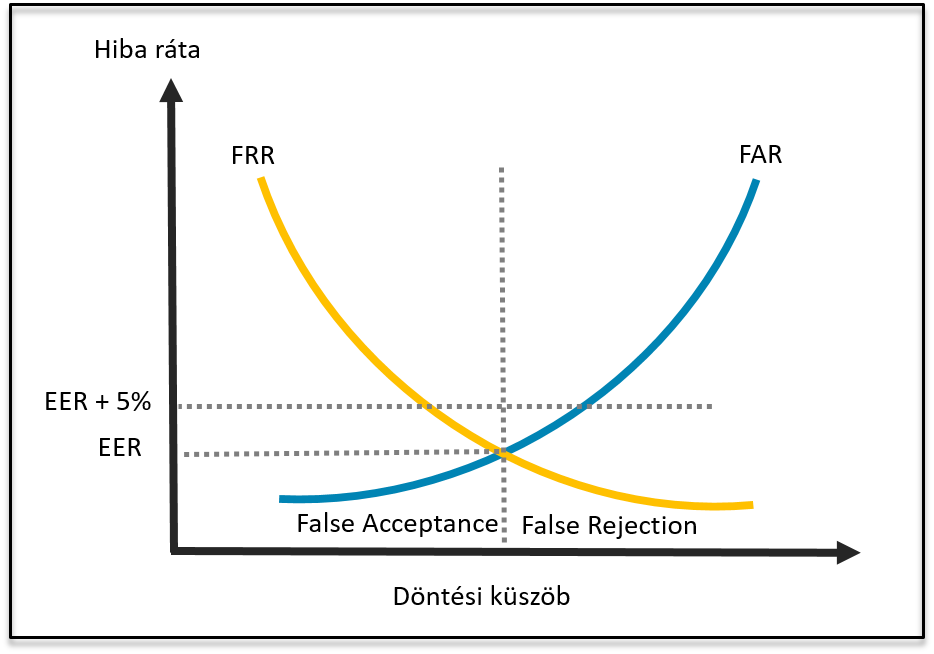
\includegraphics[width=150mm, keepaspectratio]{figures/eer.png}
	\caption{Biometrikus rendszerek karakterisztikája.}
	\label{fig:eer}
\end{figure}
\ \\
Az EER minimalizálásával tehát maximalizáljuk a biometrikus rendszer teljesítményét abból a szempontból, hogy a lehetséges hibák száma így a legkevesebb.
\newpage
\section{Beszélőfelismerés}

Az emberi kommunikáció során fontos feladat a beszélő partner felismerése. A telekommunikációs technológia fejlődése miatt elterjedt a telefonon vagy interneten történő hangalapú kommunikáció; a telefonos felhasználófelismerés mint biometrikus azonosítási módszer megjelent már banki alkalmazásokban, call centerekben és az elektronikus kereskedelemben is (mobiltelefonos vásárlás). Az elektronikus kommunikáció során sokszor csak a beszélő hangjára hagyatkozhatunk, az alapján ismerhetjük fel az illetőt. A beszélőfelismerést háromféle módon végezhetjük~\cite{taufiq_2015}:

\begin{itemize}
	\item Naiv beszélőfelismerés: Az emberi, naiv beszélőfelismerés során az ismerős hangokat meglepően nagy pontossággal ismerjük fel.
	\item Törvényszéki beszélőfelismerés: A törvényszéki szakértői vizsgálat eredménye.
	\item Automatikus beszélőfelismerés: A beszélőfelismerést számítógépes rendszer végzi.
\end{itemize}

A beszélőfelismerés alatt három szűkebb fogalmat értünk. Ha a folyamat során az ismeretlen beszélőről azt ellenőrizzük, hogy az-e akinek állítja magát beszélő ellenőrzésről van szó. Beszélő szegmentáláskor a hangmintát homogén csoportokra bontjuk a beszélő személye alapján. Végül beszélő azonosításról beszélünk, ha az illető hangját rögzített hangok egy csoportjával vetjük össze és azt szeretnénk eldönteni, hogy melyikhez hasonlít a legjobban. Utóbbi felveti a kérdést, hogy mi történik ha a beszélő nem tagja a csoportnak.
\newline
\newline
Emiatt megkülönböztetjük a nyitott és zárt halmazú beszélőazonosítást. Utóbbi esetén csak olyan beszélőket ismerünk fel, akikről van hangminta az adatbázisban, míg az előbbinél ismeretlen beszélők is megjelenhetnek, így ezt is kezelni kell.
\newline
\newline
A beszélőfelismerés továbbá lehet szövegfüggő és szövegfüggetlen attól függően, hogy a felismerő rendszer egy előre meghatározott mondatot vár, vagy bármilyen hangminta alapján képes elvégezni a felismerést.

\section{Az automatikus beszélőfelismerés története}

Az automatikus beszélőfelismerést egy számítógépes program végzi emberi beavatkozás nélkül. Az első automatikus beszédfelismerő rendszert a Texas Instruments fejlesztetése volt és 1977-ben publikálták~\cite{Shaver2016ABR}. A rendszer szövegfüggő beszélőellenőrzésre volt képes és az évek során a téves elutasítási és elfogadási rátája 1$\%$ alatt maradt. A hetvenes évek óta a beszélőazonosító és ellenőrző rendszerek rengeteget fejlődtek kezdve a vektor kvantálástól a GMM modelleken át a mély neurális hálókig.

\begin{figure}[!ht]
	\centering
	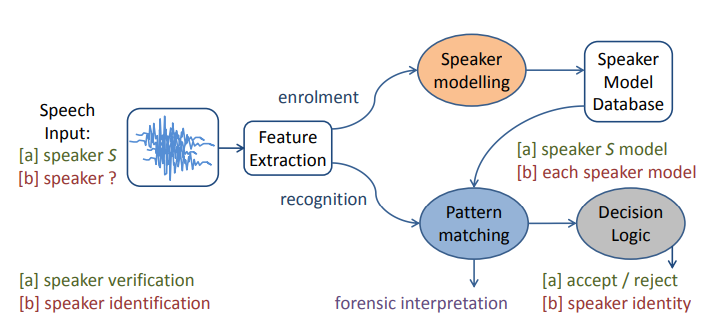
\includegraphics[width=150mm, keepaspectratio]{figures/automatic_speaker_recognition.png}
	\caption{Korábbi automatikus beszélőfelismerő rendszerek architektúrája~\cite{finnian_2014}.}
	\label{fig:automatic_speaker_recognition}
\end{figure}
\ \\
Az automatikus beszélőfelismerő általános működését a \ref{fig:automatic_speaker_recognition} ábra szemlélteti. Működését tekintve két fázist különböztetünk meg: A regisztrációs vagy felvételi fázisban hangmintát veszünk a felhasználótól~\cite{finnian_2014}. Később az azonosítási vagy ellenőrzési fázisban a rendszer újabb mintát kér és az előbbi fázisban eltárolt hangmintával hasonlítja össze. 
\newline
\newline
Mindkét fázis során az első lépés rögzített, alacsonyabb dimenziós \emph{jellemzők kinyerése}, amelynek során a beszédet tömörebb formára hozzuk (pl. hangvektor). Az első, \emph{regisztrációs fázisban} ezután statisztikai modelleket készít az egyes beszélőkhöz a kinyert jellemzők alapján, amelyeket eltárol a beszélő adatbázisban. Ebben a fázisban egy küszöbérték is meghatározásra kerül. \emph{ellenőrzési fázisban} a rendszer kinyeri ugyanazokat a jellemzőket az aktuális hangmintából, majd egy \emph{mintaillesztés} nevű eljárással összehasonlítja a korábban tárolt modellt a jellemzőkkel. Az összehasonlítás eredményét és a küszöbértéket figylembe véve a rendszer dönt az azonosítás vagy ellenőrzés eredményéről.

\begin{enumerate}
	\item beszélő-ellenőrzés esetén megkeresi az ellenőrizendő személyhez tartozó modellt az adatbázisban és összehasonlítja az aktuális jellemzőkkel. Ha az eredmény a küszöbszint felett van, a rendszer egyezést mutat.
	\item beszélőazonosítás esetén az aktuális jellemzőket az összes modellel összehasonlítja, majd a legjobb egyezés mellett dönt. 
\end{enumerate}

\subsection{Jellemző kinyerés}
A jellemző kinyerés célja a dimenzió csökkentése és a beszélőspecifikus információk kinyerése. Mivel a beszéd komplex jel, a beszélő azonosítása szempontjából felesleges információkat is hordoz. Ilyen például a környezet és a csatorna zaja. A kinyert jellemzőket a hangminta terjedelme alapján osztályozzuk. \emph{Rövidtávú jellemzők} a 20-30 ms-os keretekből kinyert mel-frekvenciás és lineáris prediktív kepsztrális együtthatók (MFCC és LPCC)~\cite{taufiq_2015}. A \emph{prozódikus jellemzők} kinyerése 100 ms-os terjedelemben történik és a beszéd ritmusát, a hangmagasságot és a sebességet jellemzik. A hosszútávú jellemzőket a jel akár perc hosszú kereteiből nyerjük ki. Ezek képesek reprezentálni a beszélő akcentusát illetve a szavak szemantikáját és az idiolektust.
\newline
\newline
A beszélőfelismerő rendszerek teljesítményét javította, ha a jellemzőket csak
a hangminta azon részeiből nyerték ki, amikben beszéd is volt. Erre alkalmazott technika a \emph{Voice Activation Detection} (\emph{VAD}).

\subsection{Jellemző normalizálás}

Jellemzőkinyerés során próbáljuk kiszűrni a beszélő szempontjából értékes részéket, ugyanakkor nincs tökéletes jellemző, amely ne változna a környezet hatására. Ezt a változást segítik minimalizálni a normalizálási módszerek.

\subsection{A beszélőfelismerő modellek története}

Kezdetben a vektor kvantálás volt az elterjed modellezési módszer, amit később a \emph{Gaussian Mixture Model} (\emph{GMM}) váltott fel. A GMM egy adathalmazt több normális eloszlás keverékeként ír le és képes nem felügyelt módon klaszterezni az adatokat. Egy beszélőhöz egy valószínűségi sűrűségfüggvényt rendel, amely különböző pontokban kiértékelve (például teszt fázisban a beszélőtől kinyert jellemzők) egy valószínűséget ad a két beszélő hasonlóságára~\cite{taufiq_2015}.
\newline
\newline
A GMM megközelítés főleg beszélőazonosításra alkalmas. Beszélő-ellenőrzéshez szükség volt egy másik modellre is, ami képes leírni minden más beszélőt az ellenőrizendőn kívül. Erre adott megoldást az \emph{Universal Background Model} (\emph{UBM}). Később jobb teljesítményt értek el, ha a teszt fázisban a beszélőkkel először UBM modelleket tanítottak és ezekből származtattak GMM-eket. Ezt nevezik GMM-UBM módszernek.
\newline
\newline
Mivel a tanító és teszt hangminták eltérő hosszúságúak lehetnek, szükség volt egy fix hosszúságú reprezentációra, ezt oldották meg a GMM szupervektorok, amelyeket az akkori megközelítés szerint szupport-vektor gépekkel vagy faktoranalízissel használtak.
\newline
\newline
Az utóbbi két módszer előnyeit kombinálva megszületett az $i-vektorok$, amelyet követve eljutunk a mai state-of-the-art módszerhez, a mély neurális hálózatokhoz (DNN).

\section{Korábbi eredmények}

A \ref{fig:previous_identification_results} ábra korábbi eredményeket mutat szövegfüggetlen beszélőfelismerő rendszerekről. Megfigyelhető, hogy főleg tízes, százas nagyságrendű beszélővel tanított, zárt-halmazú rendszerekről van szó és a tanító mintákat is többnyire laboratóriumi körülmények között rögzítették. A pontosságot ennek fényében kell értelmezni.

\begin{table}[!ht]
	\resizebox{\textwidth}{!}{%
	\begin{tabular}{*7l} \toprule
		\bfseries Szerző (év)
		& \bfseries Szervezet
		& \bfseries Adatbázis
		& \bfseries Módszer
		& \bfseries Jellemzők
		& \bfseries \begin{tabular}{@{}l@{}} Hang \\ típusa \end{tabular}
		& \bfseries Pontosság \\ \midrule
		
		\begin{tabular}{@{}l@{}} Douglas A. Reynolds  \\  (1995) \end{tabular}
		& \begin{tabular}{@{}l@{}} Lincoln  \\  Laboratory \end{tabular}
		& 49
		& MFCC 
		& \begin{tabular}{@{}l@{}} rövid \\ kifejezések \end{tabular} 
		& telefon 
		& 96.8 \% \\
		
		\begin{tabular}{@{}l@{}} Rabah W.  \\  (2004) \end{tabular}
		& \begin{tabular}{@{}l@{}} King Abdulaziz  \\  University \end{tabular}
		& 20
		& \begin{tabular}{@{}l@{}} SVD-alapú   \\  algoritmus \end{tabular}
		& LPC/Cepstral
		& iroda
		& 94 \% \\
		
		\begin{tabular}{@{}l@{}} Yang Shao  \\  (2008) \end{tabular}
		& \begin{tabular}{@{}l@{}} Ohio State  \\  University \end{tabular}
		& 34 
		& GFCCs 
		& hallási jellemzők
		& telefon
		& \~{}99.33 \% \\
		
		\begin{tabular}{@{}l@{}} P. Krishnamoorthy  \\  (2011) \end{tabular}
		& TIMIT
		& 100 
		& GMM-UBM 
		& MFCC
		& labor
		& 80 \% \\
		
		\begin{tabular}{@{}l@{}} Alfredo Maesa  \\  (2012) \end{tabular}
		& Voxforge.org
		& 250 
		& MFCC 
		& \begin{tabular}{@{}l@{}} spektrális \\ jellemzők \end{tabular} 
		& \begin{tabular}{@{}l@{}} beszéd- \\ adatbázis \end{tabular} 
		& > 96 \% \\

		\begin{tabular}{@{}l@{}} Sharada V. Chougule  \\  (2015) \end{tabular}
		& \begin{tabular}{@{}l@{}} Finolex Academy  \\  of Management \\ and Technology \end{tabular}
		& 97 
		& NDSF 
		& spektrális
		& labor
		& \~{}98-100 \% \\
		
	\bottomrule
	\end{tabular}}
	\centering
	\caption{Korábbi eredmények szövegfüggetlen beszélőazonosítás terén 2017 előtt~\cite{singh_2017}.}
	\label{fig:previous_identification_results}
\end{table}

\newpage

\section{Modern beszélőfelismerés}

A következő fejezetben bemutatom a 2017-2019-ben publikált korszerű beszélőfelismerő rendszereket és az általuk elért eredményeket. Mivel ez a kutatási terület jelenleg népszerű és folyamatosan újabb eredményeket érnek el, a bemutatott rendszereket a hivatkozások száma, a dátum és a \emph{www.paperswithcode.com} oldal rangsorolása alapján választottam ki.
\newline
\newline
Az eredmények általános összehasonlítása több ok miatt is nehéz feladat. A cikkekben a legjobb eredmények feltüntetése miatt relatív eredményeket tartalmaznak egy-egy korábban
publikált rendszerhez képest. Ezen kívül változik, hogy zárt vagy nyílt-halmazú beszélőfelismerésről, beszélő azonosításról vagy beszélő-ellenőrzésről van-e szó. Változik maga a teszthalmaz nehézsége is: etnikai, nemi, foglalkozásbeli diverzitás, a hangminták hossza, a hangfelvétel minősége, van-e irreleváns zaj, stb. Továbbá
a legtöbb cikk nem biztosít letölthető modellt, konfigurációt, szkripteket az előfeldolgozáshoz, így azonos környezethez reprodukálni kellene őket.


\subsection{Deep Speaker: an End-to-End Neural Speaker Embedding (2017) System~\cite{deep_speaker}}

A Deep Speaker egy neurális hálózatokon alapuló embedding rendszer. Az \emph{embedding} kifejezés alatt valamilyen leképzést értünk. Például amikor hangokból hangvektorokat készítünk. A rendszer a hangmintákat egy hipergömbre vetíti, ahol azoknak a hasonlóságát koszinusz távolsággal méri.
\newline
\newline
A leképzések előnye, hogy felhasználástól függetlenek, módszertől függően használhatók beszélőazonosításra, identifikációra és diarizációra is. 
\newline
\newline
Jellemző kinyerésre ResNet és GRU (LSTM változat) architektúrákkal próbálkoztak. Tanításhoz \emph{triplet loss} veszteséget használtak, és a hangvektorok között koszinusz távolságot számoltak.
\newline
\newline
A Deep Speaker által elért eredményeket a korábbi legkorszerűbb \emph{i-vektoros} rendszerekhez mérték.
Ezeknek az általános felépítése a következőképpen néz ki:
\begin{itemize}
	\item Statisztikák gyűjtése
	\item i-vektorok leképzése (jellemző kinyerés)
	\item osztályozás (PLDA)
\end{itemize} 
Ezek a rendszerek GMM-UBM modellt használtak a statisztikák kinyerésére, amiket jellemzőkkel (pl. MFCC) optimalizáltak. A GMM-UBM helyett később
DNN alapú megoldással is próbálkoztak. A GMM-UBM kimeneteként kapott
sokdimenziós statisztikákat ezután alacsony dimeziójú i-vektorokká alakítják, amit aztán PLDA modellel osztályoznak és verifikációra használják.
Jelenleg a mai korszerű rendszerek az első két lépést összevonják és CNN-eket használnak alacsony dimenziós jellemzőkinyerésre.
\begin{table}[!ht]
	\begin{tabular}{*3l} \toprule
		\bfseries Rendszer & \bfseries EER (\%) & \bfseries ACC (\%) \\ \midrule
		DNN i-vector baseline & 13,79 & 51,72 \\
		\rowcolor{gray!10}
		ResCNN, softmax & 6,13 & 81,95 \\
		ResCNN, triplet & 2,69 & 86,21 \\
		\rowcolor{gray!10}
		ResCNN, softmax (pre-train) + triplet & 2,23 & 90,53 \\
		GRU, softmax & 5,42 & 83,05 \\
		GRU, triplet & 3,23 & 84,19 \\
		\rowcolor{gray!10}
		GRU, softmax (pre-train) + triplet & 2,77 & 89,50 \\
		\bottomrule
		\hline
	\end{tabular}
	\centering
	\caption{Mandarin nyelvű szöveg-független azonosítás eredményei tanításra és tesztelésre a Train50k és Eva200 adathalmazokat használva.}
	\label{fig:deep-speaker-independent-mandarin-results}
\end{table}
\newpage
\ \\
A legjobb architektúrának a \emph{ResCNN} bizonyult softmax előtanítással és triplet lossal tanítva. Ezzel a \ref{fig:deep-speaker-independent-mandarin-results} szerint Eva200 adathalmazon \emph{90,53\%}-os eredményt értek el. A Train50k, Train250k és Eva200k az UID adathalmaz részei.

\begin{table}[!ht]
	\begin{tabular}{*3l} \toprule
		\bfseries Rendszer & \bfseries EER (\%) & \bfseries ACC (\%) \\ \midrule
		ResCNN on Train50k & 2,23 & 90,53 \\
		\rowcolor{gray!10} 
		ResCNN on Train250k & 1,83 & 92,58 \\
		GRU on Train50k & 2,77 & 89,50 \\
		\rowcolor{gray!10} 
		GRU on Train250k & 2,35 & 90,77 \\
		\bottomrule
		\hline
	\end{tabular}
	\centering
	\caption{Szöveg-független azonosítás eredményei.}
	\label{fig:deep-speaker-independent}
\end{table}
\ \\
A \ref{fig:deep-speaker-independent} szerint pedig nagyobb adathalmazzal való tanítás nagyobb pontosságot és alacsonyabb EER-t eredményezett. A legjobb eredményt a RestCNN-el érték el Train250k-val tanítva.
\newline
\newline
Az eredmények a korábbi i-vektoros rendszerekhez képest a Deep Speaker 50\% csökkentette az EER-t, és pontosságban 60\%-os javulást ért el.

\subsection{Speaker Recognition from Raw Waveform with SincNet (2018)~\cite{sincnet}}

A SincNet is a korábban használt i-vektoros rendszerek helyett mutat be egy új CNN hálózatot. A CNN-ek előnye, hogy a korábban használt kézzel fabrikált jellemzők (pl. MFCC) helyett a hálózat maga tanulja meg a hang alacsony szintű reprezentációját nyers hullámformákból. Mivel a cikk a CNN-t kiegészíti hangszűrőkkel és a jelfeldolgozásban használatos fogalmakat használ, először ismertetem ezeket:
\begin{itemize}
	\item Beszéd frekvencia: Egy periodikus hullámforma esetében a frekvencia a periódusidő reciproka, azza megmondja, hogy egységnyi idő alatt hány periódus ment végbe. Az emberi hang esetében a komplex hullámforma Fourier analízissel felbontható trigonometrikus (periodikus) függvények összegére. A Fourier transzformáció segítségével az idő-amplitúdó doménből frekvencia-amplitúdót képzünk, így a frekvencia komplex jel esetén és értelmet nyer.
	\item Sávszélesség: Hang esetében általánosan a legalacsonyabb és legmagasabb frekvencia közötti különbség.
	\item Cutoff frekvencia: A hangszűrők legfontosabb paramétere. Például aluláteresztő szűrő esetében a cutoff fölötti frekvenciákat a szűrő tompítja, nem engedi át.
	\item Band pass filter: Olyan szűrő, ami csak a cutoff frekvencia környezetében lévő frekvenciákat engedi át (egy alul -és felüláteresztő szűrő kombinációja).
\end{itemize} 
\ \\
\newline
A SincNet egy új CNN architektúra, amelyben az első réteg ún. paraméterezhető sinc függvényekkel van kiegészítve, amelyek band pass szűrőket implementálnak.
\newline
\newline
A korábban használt kézzel fabrikált jellemzők, mint az MFCC vagy FBANK esetében semmi sem garantálja, hogy optimálisak minden beszélőfelismerő feladatra. A cikk szerint lehetséges, hogy ezek a jellemzők nem veszik figyelembe a hangmagasságot és a formánsokat. A feltevésük szerint hullámforma feldolgozásánál a legfontosabb a CNN első rétege. Ezért a SincNet a hullámformákat sinc függvényekkel konvolválja, amelyek paraméterei az alacsony és magas cutoff frekvencia.

\begin{figure}[!ht]
	\centering
	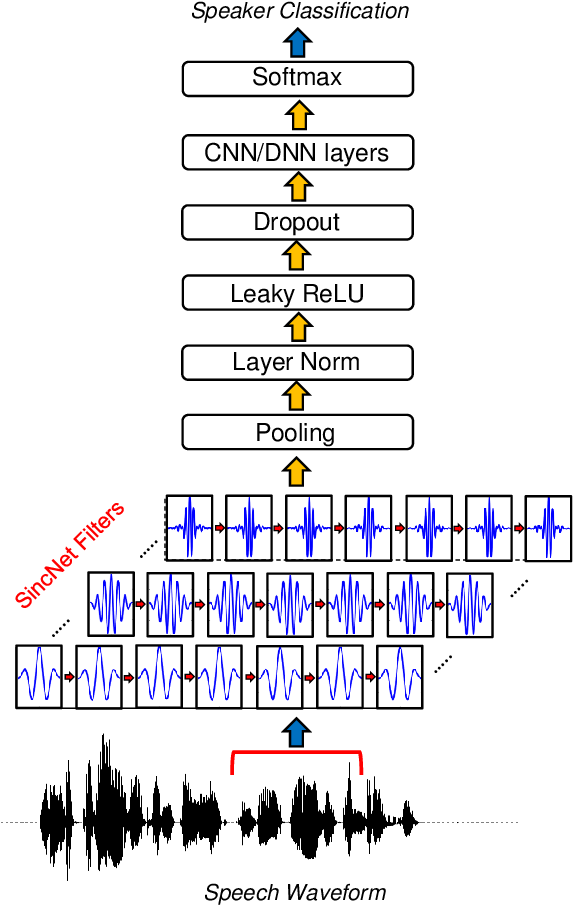
\includegraphics[width=120mm, keepaspectratio]{figures/sincnet-nn.png}
	\caption{SincNet architektúra~\cite{sincnet}.}
	\label{fig:sincnet-nn}
\end{figure}
\ \\
\newline
A SincNetet a TIMIT (462 beszélő) és Librispeech (2484 beszélő) adatbázisokkal tanították.
A beszédminták elejéről a szüneteket eltávolították, és LibriSpeech esetén azokat a mintákat, amelyek tartalmaztak legalább 125 ms hosszú szünetet, annak mentén feldarabolták. A TIMIT adatbázisnál egy beszélőtől 5 mintával tanítottak és 3 mintával teszteltek, míg LibriSpeechnél véletlenszerűen választottak 12-16 másodperces mintákkal tanítottak és 2-6 másodpercesekkel teszteltek.
\newline
\begin{table}[!ht]
	\begin{tabular}{*3l} \toprule
		\bfseries Rendszer & \bfseries TIMIT & \bfseries LibriSpeech \\ \midrule
		DNN-MFCC & 0,99 & 2,02 \\
		\rowcolor{gray!10} 
		CNN-FBANK & 0,86 & 1,55 \\
		CNN-Raw  & 1,65 & 1,00 \\
		\rowcolor{gray!10} 
		SINCNET & 0,85 & 0,96 \\
		\bottomrule
		\hline
	\end{tabular}
	\centering
	\caption{Szöveg-független azonosítás eredményei adatbázisok szerint.}
	\label{fig:sincnet-identification}
\end{table}
\ \\
A \ref{fig:sincnet-identification}-es táblázat a CER (Classification Error Rate [\%]) hiba rátát mutatja. E szerint a SincNet jobban teljesít az MFCC, FBANK és nyers hullámformákkal tanított CNN-eknél mindkét adatbázis esetében, bár látható, hogy a sima CNN és a SincNet között minimális a különbség.
\newline
\begin{table}[!ht]
	\begin{tabular}{*3l} \toprule
		\bfseries Rendszer & \bfseries d-vector & \bfseries DNN-class \\ \midrule
		DNN-MFCC & 0,88 & 0,72 \\
		\rowcolor{gray!10} 
		CNN-FBANK & 0,60 & 0,37 \\
		CNN-Raw  & 0,58 & 0,36 \\
		\rowcolor{gray!10} 
		SINCNET & 0,51 & 0,32 \\
		\bottomrule
		\hline
	\end{tabular}
	\centering
	\caption{Szöveg-független ellenőrzés (verifikáció) eredményei.}
	\label{fig:sincnet-verification}
\end{table}
\ \\
\newline
A SincNettel nem jellemző vektorokat képeztek és a köztük lévő távolságot használták a hasonlóság mérésére, hanem osztályozással használják. Ebben az esetben zárt-halmazú beszélőazonosításról beszélünk. Ez sokkal kevésbé flexibilis, mert új beszélő esetén mindig újra kell tanítani a hálózatot, de cserébe jobb teljesítményre képes. A \ref{fig:sincent-verification} ábrán egy d-vector nevű hangvektorokat képző neurális hálózatot hasonlítottak össze a SincNettel. Beszélőellenőrzés esetén a SincNet sokkal jobb EER-t ért el.
\newpage
\subsection{VoxCeleb2: Deep Speaker Recognition (2018)~\cite{voxceleb2}}

A VoxCeleb1 és VoxCeleb2 nagy méretű, beszélőfelismerés céljából készült adatbázisok. Az előbbi több mint 1000, utóbbi pedig több mint 6000 hangmintát tartalmaz hírességektől. Az adatbázisok felépítésének részleteit a \ref{voxceleb1} és \ref{voxceleb2} fejezetek ismertetik. Mindkét adatbázissal végeztek méréseket különböző neurális hálózatokkal, de a legjobb eredményeket illetve nyílt-halmazú beszélőfelismerést a VoxCeleb2-vel érték el.
\newline
\newline
Bemutatják a VGGVox nevű CNN alapú neurális hálózatot, amelyet spektrogramokkal tanítottak és hangvektorokat hoz létre. Előnye ennek a megoldásnak, hogy nyílt-halmazú beszélőfelismerésre használható, új beszélő esetén nem szükséges újra tanítani a hálózatot. 
\newline
\newline
Módosított VGG-M és ResNet architektúrákkal kísérleteztek. A modelleket contrastive loss veszteségfüggvénnyel tanították és előtanításra egy softmax réteget használtak keresztentrópiával, ami javította a modell teljesítményét. Tanító adathalmaznak a VoxCeleb2 adatbázist használták és a tesztelést a VoxCeleb1-el végezték. A méréseket EER és a \ref{eq:cdet} detektálási költség függvény szerint értékelték ki,

\begin{equation} \label{eq:cdet}
C_{det} = C_{miss} \cdot P_{miss} \cdot P_{target} + C_{fa} \cdot P_{fa} \cdot (1 - P_{target})
\end{equation}

ahol \emph{C\_miss} és \emph{C\_fa} alkalmazás specifikus paraméterek a hamis negatív és hamis pozitív hibák költsége, \emph{P\_miss} és \emph{P\_fa} pedig a hibák előfordulásának valószínűségét jelzik. \emph{P\_target} annak a valószínűsége, hogy a rendszer két olyan mintát hasonlít össze, amely egy embertől származik.
\newline
\begin{table}[!ht]
	\begin{tabular}{*4l} \toprule
		\bfseries Rendszer & \bfseries Tanítóhalmaz & \bfseries $C_{min}^{det}$ & \bfseries EER \\ \midrule
		I-vectors + PLDA & VoxCeleb1 & 0,73 & 8,8 \\
		VGG-M (Softmax) & VoxCeleb1 & 0,75 & 10,2 \\
		VGG-M & VoxCeleb1 & 0,71 & 7,8 \\
		VGG-M  & VoxCeleb2 & 0,609 & 5,94 \\
		ResNet-34 & VoxCeleb2 & 0,549 & 4,83 \\
		ResNet-50 & VoxCeleb2 & 0,429 & 3,95 \\
		\bottomrule
		\hline
	\end{tabular}
	\centering
	\caption{Beszélő ellenőrzés (verifikáció) eredményei.}
	\label{fig:sincnet-verification}
\end{table}

\newpage

\subsection{Utterance-level Aggregation for Speaker Recognition in the Wild (2019)~\cite{speaker_in_the_wild}}

A cikk két fő témája egy olyan neurális hálózat létrehozása, amely képes különböző hosszúságú hangmintákból jellemző vektorokat képezni és olyan hangminták vizsgálata amelyek irreleváns zajokat is tartalmaznak.

\begin{figure}[!ht]
	\centering
	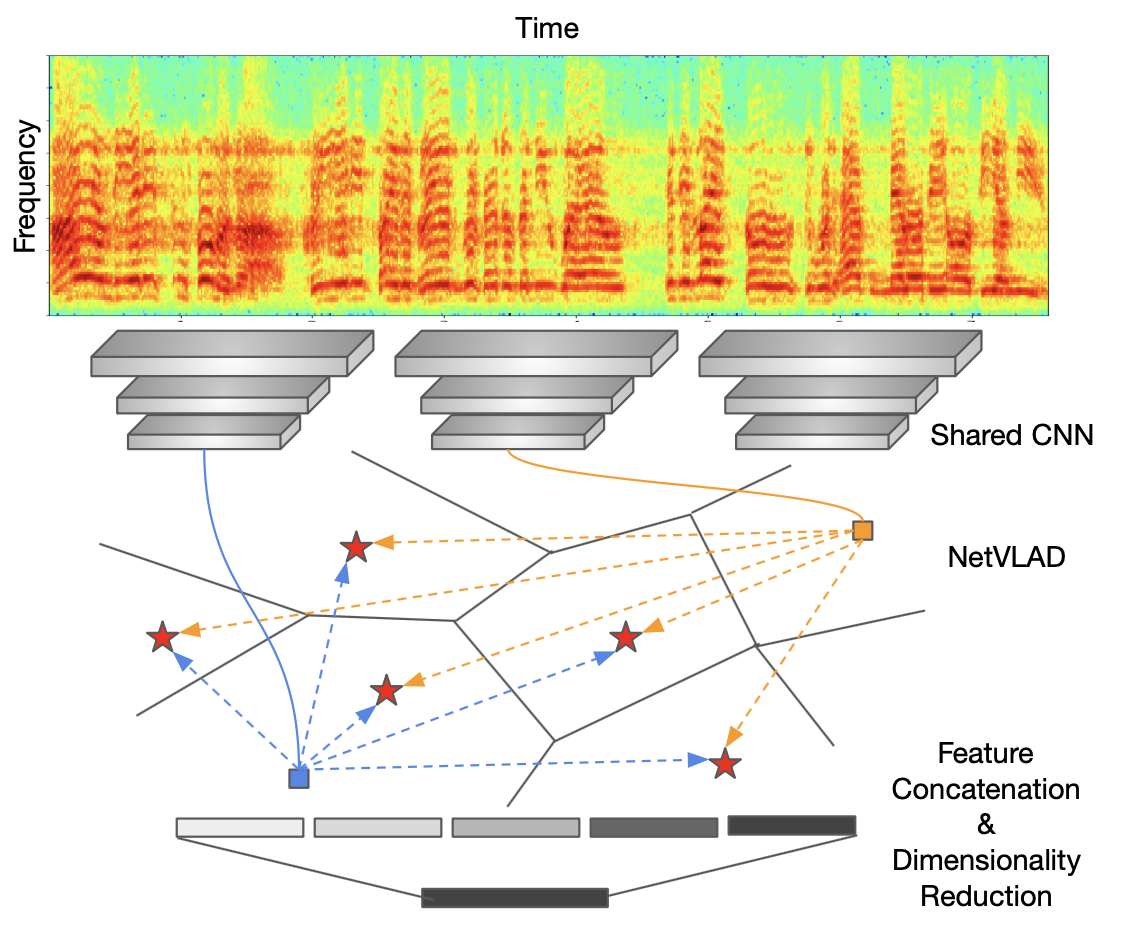
\includegraphics[width=150mm, keepaspectratio]{figures/frame-cnn.png}
	\caption{Neurális hálózat architektúra~\cite{speaker_in_the_wild}.}
	\label{fig:frame-cnn}
\end{figure}
\ \\
\newline
\newline
A hálózat három részből áll. Először egy módosított ResNet architektúrát használnak a keretszintű vektorok előállítására spektrogramokból. Az ábrán látható megosztott CNN-t hívjuk trönk hálózatnak. A keretszintű vektorok aggregálását a NetVLAD illetve GhostVLAD (Vector of Locally Aggregated Descriptors módszeren alapuló) hálózatokkal végzik. Legvégül egy FC (Fully Connected) réteget használnak a dimenzió 512-re csökkentésére.
\newline
\newline
A teljes modell end-to-end tanítására a VoxCeleb2 adatbázist használták és tesztelésként beszélőellenőrzést (verifikációt) mértek a VoxCeleb1-en.
\begin{figure}[!ht]
	\centering
	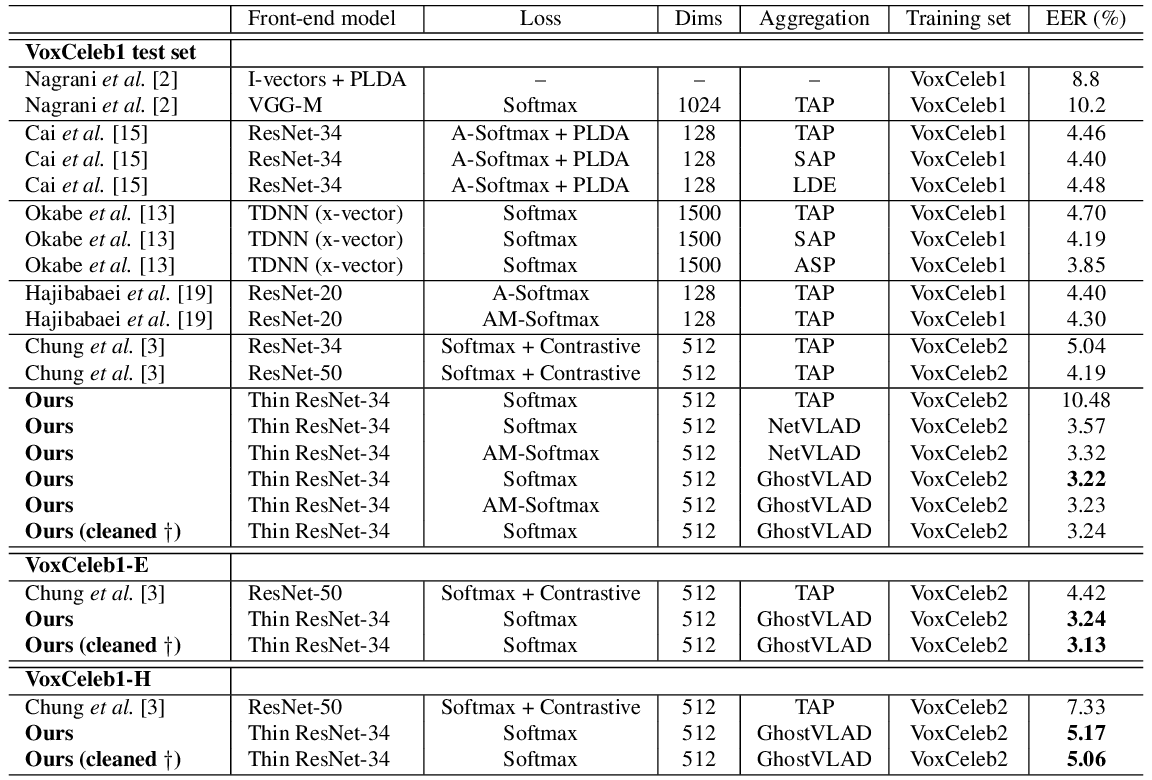
\includegraphics[width=150mm, keepaspectratio]{figures/frame-cnn-results.png}
	\caption{Neurális hálózat architektúra~\cite{speaker_in_the_wild}.}
	\label{fig:frame-cnn-results}
\end{figure}
\ \\
A \ref{fig:frame-cnn-results} táblázat mutatja a verifikációval mért EER-eket az akkori legkorszerűbb rendszerekkel szemben. Az addigiaknál lényegesen jobb EER-t értek el ezzel a módszerrel.



\chapter{Beszédadatbázisok}

A fejezet bemutatja a jelenleg ingyenes, bárki által elérhető és a tanítás során használt beszédadatbázisokat. Egy beszédadatbázis előállítása bár ránézésre egyszerű feladatnak tűnik,
valójában komplex folyamat és sok munkát igényel. Egyes adatbázisokat beszédfelismerés céljából készítettek, másokat beszélőfelismerésre. Az előbbinél a kontrollált körülmények előállítása, megfelelés egyes nyelvtani mérőszámoknak (fonémák, diádok egyenletes elosztása stb.), utóbbinál a nagyobb méret miatt az automatizmus szükségessége bonyolítja a feladatot. Ezen felül mindkét esetben a szerzői jogok védelmére is ügyelni kell. (A dolgozatban a beszédadatbázis, beszédkorpusz és beszédadathalmaz ugyanarra vonatkozik.)

\section{Beszédadatbázisok}

\subsection{TIMIT}

A TIMIT beszédkorpuszt automatikus beszédfelismerő rendszerek fejlesztéséhez tervezték. 630 beszélőtől tartalmaz mintákat amerikai angol nyelven a 8 legelterjedtebb nyelvjárásban.
A TIMIT archívum tartalmaz egy TRAIN és egy TEST mappát, ezek tanításhoz és teszteléshez valók. Ezeken belül további, a dialektusok sorszámával (DR1, ..., DR8), azon belül a beszélő azonosítójával elnevezett könyvtárak találhatók. Egy beszélőhöz
10 db beszédminta tartozik 16 kHz-es NIST SPHERE fájlok formájában~\cite{timit}.
\newline
\newline
\begin{table}[!ht]
	\begin{tabular}{*4l} \toprule
		\bfseries Dialektus regió (DR) & \bfseries Férfi & \bfseries Nő & \bfseries Összesen \\ \midrule
		1                             & 31 (63\%)      & 18 (27\%)   & 49 (8\%)          \\
		\rowcolor{gray!10} 
		2                             & 71 (70\%)      & 31 (30\%)   & 102 (16\%)        \\
		3                             & 79 (67\%)      & 23 (23\%)   & 102 (16\%)        \\
		\rowcolor{gray!10} 
		4                             & 69 (69\%)      & 31 (31\%)   & 100 (16\%)        \\
		5                             & 62 (63\%)      & 36 (37\%)   & 98 (16\%)         \\
		\rowcolor{gray!10} 
		6                             & 30 (65\%)      & 16 (35\%)   & 46 (7\%)          \\
		7                             & 74 (74\%)      & 26 (26\%)   & 100 (16\%)        \\
		\rowcolor{gray!10} 
		8                             & 22 (67\%)      & 11 (33\%)   & 33 (5\%)          \\
		\bottomrule
		\hline
	\end{tabular}
	\centering
	\caption{A beszélők eloszlása dialektusok szerint.}
	\label{fig:timit-dialects}
\end{table}
\newpage
A dialektus régiók a következők:

\begin{multicols}{2}
	\begin{itemize}
		\item DR1:  New England
		\item DR2:  Northern
		\item DR3:  North Midland
		\item DR4:  South Midland
		\item DR5:  Southern
		\item DR6:  New York City
		\item DR7:  Western
		\item DR8:  Army Brat (moved around)
	\end{itemize}
\end{multicols}
\ \\
A NIST SPHERE formátum az elején definiál egy fix hosszú fejlécet, amit a hang bináris kódolása követ. Erre figyelni kell a hangfájlok beolvasásánál, Python esetében nem minden hangfeldolgozó könyvtár támogatja. Ilyen esetben kézzel el kell távolítani a fejlécet a fájlok elejéről. A hangfájlokhoz tartozik egy szöveges dokumentum ami az elhangzott szöveget és annak a wav fájlbeli helyét tartalmazza. Továbbá egy WRD fájl írja le a szavakat és egy PHN kiterjesztésű a fonémákat, illetve azok időbeni elhelyezkedését a wav fájlban.
\newline
\newline
A hangfájlokhoz tartozó egyéb fájlok beszédfelismerés szempontjából fontosak. Mivel én a beszédkorpuszt beszélőfelismerésre használtam, csak a hangfájlokra volt szükségem. A TEST mappában -- mivel a TIMIT-et alapvetően beszédfelismeréshez tervezték -- teljesen különböző beszélők vannak a TRAIN mappához képest, ezért a TRAIN mappabeli beszélőket osztottam fel tanításhoz és teszteléshez.

\subsection{CMU Arctic}

A CMU Arctic adatbázist beszédszintézishez kapcsolódó kutatásokhoz tervezték. A beszédszintézis az emberi beszéd mesterséges, általában számítógéppel történő előállítása. Mivel akkoriban (2003) a publikusan elérhető beszédadatbázisok kis méretűek voltak, létrehozták a CMU Arcticot, ami több beszédadatbázis összessége. Egy adatbázis egy beszélőhöz tartozik és egyéb információkat is tartalmaz, mint a fonetikus kiejtés vagy a beszédjel egyes jellemzőit (pitchmark) tartalmazó fájlok~\cite{cmu_arctic}.
\newline
\newline
Mivel a CMU Arctic felhasználási célja a beszédszintézis, a felvételek studió minőségűek, mentesek külső zajoktól és a beszélő által keltett zajoktól is.
\newline
\newline
Az egyes Arctic adatbázisok közel 1150 kb. 1-4 másodperces beszédmintából állnak. Az egy beszélőhöz tartozó mintákat két azonos elemszámú A és B csoportra osztották, amelyek fonetikailag kiegyensúlyozottak. Ez azt jelenti, hogy az adott beszédmintában található fonémák körülbelül ugyanakkora gyakorisággal fordulnak elő mint az átlagos társalgás közben az adott nyelven.
A beszédminták WAV fájlok formájában 32 kHz-en lettek mintavételezve. A felvételek öt beszélőtől tartalmaznak hangmintákat:
\newline
\begin{itemize}
	\item férfi általános amerikai angol akcentus
	\item női általános amerikai angol akcentus
	\item férfi kanadai angol akcentus
	\item férfi skót angol akcentus
	\item férfi indiai angol akcentus
\end{itemize}
\bigskip
A CMU Arctic tartalmaz egy listát az egyes beszélők által felolvasott szövegekkel.
Mivel ez egy mindenki által elérhető ingyenes beszédadatbázisnak készült és szabad szoftver licensszel rendelkezik, fontos szempont volt, hogy a felolvasott szövegek ne sértsenek szerzői jogokat. Emiatt a listán szereplő mondatok a legnagyobb ingyenes, szabadon felhasználható szövegkorpuszból, a Project Gutenbergből származnak. A Project Gutenberg célja szerzői jogokat nem sértő angol nyelvű könyvek gyűjtése és elérhetővé tétele.
\newline
\newline
A CMU Arctic eleinte 2,5 millió szóból és az azokat tartalmazó 168000 mondatból állt. Ezekből a FestVox beszédszintézis projekt segítségével kiválogattak 52000 olyan mondatot, amelyek kiejtése könnyű és hossza 5 és 15 szó közé esett. További szigorításként csak olyan szavak kerülhettek be, amelyek részei a CMUDICT lexikonnak, hogy elkerüljék az eltérő kiejtéseket.
\newline
\newline
Ezután a Festvox segítségével az 52000 mondatból kiválogatták a legnagyobb diád lefedettségű halmazt. A diád két egymás utáni félhang együtteseként előálló nyelvi egység, amely lefedettségének mértéke a beszédszintézis során előállított beszéd minősége miatt fontos. 
\newline
\newline
A kiválogatott részt kivéve egy újabb halmazt választottak ki, amelyek 668 és 629 mondatból álltak. Ezeket manuálisan átnézve tovább finomították.

\begin{table}[!ht]
	\begin{tabular}{*4l} \toprule
		\bfseries Arctic & \bfseries Automatikus fázis & \bfseries Kézi finomítás I. & \bfseries Kézi finomítás II. \\ \midrule
		A halmaz                             & 668      & 597   & 593          \\
		\rowcolor{gray!10} 
		B halmaz                             & 629      & 541   & 539        \\
		Összesen                             & 1297      & 1138   & 1132        \\
		\bottomrule
		\hline
	\end{tabular}
	\centering
	\caption{Arctic CMU automatikus és kézi fázisok.}
	\label{fig:arctic-phases}
\end{table}
\ \\
A CMU Arctic diád lefedettsége 80\% és az előbbihez hasonlóan triád lefedettsége 14\%. Az előbbi megelőzi a TIMIT beszédkorpuszban lévő diád lefedettséget, utóbbiban viszont a TIMIT jobb a több (2343) mondat miatt.

\begin{table}[!ht]
	\begin{tabular}{*8l} \toprule
		\bfseries Corpus & \bfseries Mondat & \bfseries Szó & \bfseries Fonéma  & \bfseries \begin{tabular}{@{}l@{}} Fonéma \\ lefedettség \end{tabular}  & \bfseries \begin{tabular}{@{}l@{}} Diád \\ lefedettség \end{tabular}  & \bfseries \begin{tabular}{@{}l@{}} Triád \\ lefedettség \end{tabular} \\ \midrule
		TIMIT-all & 2342 & 20771 & 87819 & 100\% & 78,2\% & 19,4\% \\
		\rowcolor{gray!10} 
		Arctic & 1132 & 10045 & 39153 & 100\% & 79,6\% & 13,7\% \\
		\bottomrule
		\hline
	\end{tabular}
	\centering
	\caption{Arctic CMU vs. TIMIT.}
	\label{fig:arctic-vs-timit}
\end{table}

\subsection{LibriSpeech}

2015-ben már vizsgálták a hangoskönyvek beszédszintézishez való használatát és léteztek ilyen célú beszédadatbázisok, de nem volt automatikus beszédfelismerés céljára létrehozott, ingyenes, mindenki által elérhető beszédkorpusz. A LibriSpeech beszédfelismerő rendszerek tanítására és kiértékelésére készült. Tartalma a LibriVox projektből származik, amelynek célja szabadon terjeszthető hangfelvételek készítése ingyenes, közkinccsé vált könyvekről, és ezek közzététele bárki számára az interneten~\cite{librispeech}.
\newline
\newline
A projekt körülbelül 1000 órányi beszédet tartalmaz 16 kHz-en mintavételezve. Tartalmaz ezek mellett több előre tanított beszédfelismerő modellt és Kaldi szkripteket beszédfelismerő rendszerek készítéséhez.
\newline
\newline
Az előfeldolgozási fázisban a könyvek szövegét normalizálták; kis és nagybetűk helyett csak nagybetűket használtak, eltüntették az írásjeleket és a gyakori rövidítéseket teljes szavakkal helyettesítették. Ezután a hangmintákat felismertették a Kaldi \emph{gmm-decode-faster} dekóderével, amihez egy VoxCeleb adatbázison tanított modellt használtak.
\newline
\newline
Összemérték az előbbi modell által felismert szöveget az eredeti írással és azokat a részeket választották ki, ahol a kettő megegyezett. A hanganyagot legfeljebb 35 másodperces részekre tördelték minimum 0.5 másodperces szünetek mentén.
\newline
\newline
A következő fázisban egy fMMRl (HMM-alapú) modellel ismét összemérték a felismert szöveget a valódival. Ez okozott hamis pozitív eredményeket is, de az audioanyag mennyisége miatt elhanyagolható volt. Ez a fázis tehát 35 másodperces nagy valószínűséggel helyesen transzkriptált anyagokat tartalmazott.
\newline
\newline
A harmadik fázis ezeknek az apróbb szegmensekre tördelése volt, amit két módszerrel végeztek el. Tanítóadatok esetén minden olyan szünetnél tördeltek, ahol az legalább 0,3 másodperc hosszú volt. Tesztadatok esetén csak ott tördeltek, ahol ez a szünet egybeesett a mondat végével is.

\begin{table}[!ht]
	\begin{tabular}{*6l} \toprule
		\bfseries Részhalmaz & \bfseries Óra & \bfseries beszélő / perc & \bfseries \begin{tabular}{@{}l@{}} Férfi \\ beszélő \end{tabular}
		& \bfseries \begin{tabular}{@{}l@{}} Női \\ beszélő \end{tabular} & \bfseries \begin{tabular}{@{}l@{}} Összes \\ beszélő \end{tabular} \\ \midrule
		dev-clean & 5,4 & 8 & 20 & 20 & 40 \\
		\rowcolor{gray!10} 
		test-clean & 5,4 & 8 & 20 & 20 & 40 \\
		dev-other & 5,3 & 10 & 16 & 17 & 33 \\
		\rowcolor{gray!10} 
		test-other & 5,1 & 10 & 17 & 16 & 33 \\
		train-clean-100 & 100,6 & 25 & 125 & 126 & 251 \\
		\rowcolor{gray!10}
		train-clean-360 & 363,6 & 25 & 439 & 482 & 921 \\
		train-other-500 & 496,7 & 30 & 564 & 602 & 1166 \\
		\bottomrule
		\hline
	\end{tabular}
	\centering
	\caption{LibriSpeech részhalmazok.}
	\label{fig:librispeech-subset}
\end{table}
\ \\
Az audiófelvételek válogatásához a LibriVox API segítségével szereztek információkat a felolvasóról,
hogy mely hangoskönyvekben olvastak fel milyen fejezeteket, a kapcsolódó referencia szövegeket pedig a Project  Gutenbergből és az Internet Archiveból nyerték ki. A \emph{train}, \emph{dev} és \emph{test} részhalmazok között fontos, hogy ne legyen átfedés, tehát ugyanaz az olvasó csak egyetlen halmazban olvasson ezek közül. Ehhez a válogatáson kívül további óvintézkedésként kivették a többszereplős fejezeteket és lefuttaták a LIUM beszélő szegmentáló toolkitet ennek detektálására.
\newline
\newline
A tanítóhalmazba válogatott részeket három részre osztották. Ezek egyenként 100, 360 és 500 órányi audiofelvételt tartalmaznak. Az első kettőbe automatikus módszerrel az amerikai angol akcentushoz hasonló részeket válogatták bele. Egy egyszerű, a Wall Street Journal si-84 adatbázison tanított akusztikus modellt használtak a LibriSpeechen beszédfelismerésre. Ezáltal meghatározták és rangsorolták a beszélőket a Word Error Rate (a modell által hibásan felismert szavak) szerint. Az alacsonyabb WER pontszámmal rendelkező olvasók a \emph{clean}, a magasabbal az \emph{other} részhalmazokba kerültek.

\subsection{VoxCeleb1} \label{voxceleb1}

A beszélőfelismerésre használt adatbázisok kontrollált körülmények között felvett audio anyagot tartalmaznak és kézzel válogatottak, emiatt kis méretűek. Kontrollált körülmény alatt értjük a studioban felvett, külső és belső zajoktól mentes hanganyagot. Ezek a valós körülmények közötti, azaz zajos környezetben elhangzó beszédfelismerést megnehezítik. A VoxCeleb készítői a beszélőfelismerő adabázisok automatikus létrehozására terveztek egy folyamatot és létrehozták, valamint ingyenesen elérhetővé tették a VoxCeleb beszédadatbázist, ami valós körülmények közötti hangfelvételeket tartalmaz~\cite{voxceleb1}.
\newline
\newline

\begin{table}[!ht]
	\begin{tabular}{*4l} \toprule
		\bfseries Név & \bfseries Körülmények & \bfseries Beszélők száma & \bfseries Minták száma \\ \midrule
		ELSDSR                             & Kontrollált & 22     & 198          \\
		\rowcolor{gray!10} 
		Forensic Comparison                & Telefonos   & 552   & 1264        \\
		SITW                           & Multimédia        & 299   & 2800        \\
		\rowcolor{gray!10} 
		VoxCeleb                           & Multimédia        & 1251   & 153516        \\
		\bottomrule
		\hline
	\end{tabular}
	\centering
	\caption{Beszédadatbázisok beszédfelismerés.}
	\label{fig:speaker-recognition-datasets}
\end{table}
\ \\
A VoxCeleb több mint 100000 olyan beszédmintát tartalmaz 1251 hírességtől, amik YouTube videókból származnak. Az adatbázisban a nemek aránya kiegyensúlyozott (férfiak 55\%, nők 45\%), a beszélők különböző származásúak, korúak illetve eltérő akcentussal rendelkeznek. A beszéd általában publikus eseményekről származik, így a háttérzaj, egyéb beszélők és a felvevő eszköz minősége zajossá teszi azt.
\newline
\newline
Az adatbázis előállítása a következő módon történt:
\begin{itemize}
	\item A beszélő jelöltek kiválasztása:  Olyan hírességeket válogattak akik benne vannak a VGG adathalmazban, ami 2622 híres (interneten sokat keresett) ember arcát tartalmazza.
	\item YouTube videók letöltése: Letöltötték a kiválasztott emberekhez tartozó első 50 YouTube videót. A keresés az illető nevét és utána az \emph{interview} szót tartalmazta, hogy kiszűrjék a zeneszámokat, sportfelvételeket és minél nagyobb valószínűséggel beszéljenek benne.
	\item Arcdetektálás: Az egyes videókon egy HOG-alapú arc detektorral meghatározták az arcok helyét minden egyes frameben.
	\item Aktív beszélőazonosítás: Mivel egy videóban több arc is megjelenhet egyszerre, vagy a beszélőt szinkronizálhatják, az éppen beszélő arc meghatározására illetve a szinkron kiszűrésére volt szükség. A megoldás a SyncNet volt, egy olyan kétcsatornás CNN, ami képes megbecsülni a szájmozgás és a beszéd közötti korrelációt.
	\item Arcfelismerés: Végül egy a VGG Face adathalmazzal tanított CNN segítségével ellenőrizték, hogy a beszélő arc valóban a kérdéses személy-e.
\end{itemize}

\subsection{VoxCeleb2} \label{voxceleb2}

A VoxCeleb2 ugyanúgy beszélőfelismeréshez készített, de az előző verzióhoz képest jóval nagyobb, 6112 hírességtől tartalmaz 2442 órányi beszédet tartalmazó beszédadatbázis különböző nyelvű, korú és származású beszélőkkel~\cite{voxceleb2}.
\newline
\newline
Az adatbázis előállítási folyamatot az előzőhöz képest tovább bővítették.
\begin{itemize}
	\item Duplikátum detektálás: YouTube-on gyakran feltöltik ugyanazt a videót más url alatt különböző felhasználók. Egy a VoxCeleb1 adatbázison tanított konvolúciós hálózatot használtak jellemző kinyerésre, amellyel 1024 dimenziós vektorokkal reprezentálták a beszédmintákat. Egy beszélőre kiszámolták a vektorpárok közötti Euklideszi-távolságot és ahol ez kisebb volt mint 0,1 azokat azonosnak tekintették.
	\item Nemzetiség: A beszélők nemzetiségét a Wikipediáról gyűjtötték ki egy keresőrobottal (angolul webcrawler). Ezzel a módszerrel a 6112 beszélő közül 5689 nemzetiségét sikeresen azonosították. Ebből kiderült, hogy a VoxCeleb2 etnikailag sokkal diverzifikáltabb a VoxCeleb1-hez képest, mivel a VoxCeleb1 adatbázisban jelenlévő 36 nemzetiségnél jóval többet, pontosan 145-öt tartalmaz. Ugyanakkor az amerikai angolt beszélők aránya is sokkal kisebb, 29\% a VoxCeleb1-ben mért 64\%-hoz képest.
\end{itemize}

\begin{table}[!ht]
	\begin{tabular}{*3l} \toprule
		\bfseries Adatok & \bfseries VoxCeleb1 & \bfseries VoxCeleb2 \\ \midrule
		Beszélők száma   & 1251 & 6112 \\
		\rowcolor{gray!10} 
		Beszélők száma   & 1251 & 6112 \\
		Női beszélők száma & 561 & 2351 \\
		\rowcolor{gray!10}
		Férfi beszélők száma & 690 & 3761 \\
		Videók száma & 22496 & 150480 \\
		\rowcolor{gray!10}
		Beszédminták száma & 153516 & 1128246 \\
		Átlagos videó / beszélő & 18 & 25 \\
		\rowcolor{gray!10}
		Átlagos beszédminta / beszélő & 116 & 185 \\
		Átlagos beszédminta hossz & 8,2 & 7,8 \\
		\bottomrule
		\hline
	\end{tabular}
	\centering
	\caption{VoxCeleb1 vs. VoxCeleb2.}
	\label{fig:voxceleb1-vs-2}
\end{table}

\chapter{Neurális hálózat alapú beszélőfelismerő rendszerek}

Ebben a fejezetben bemutatom a legújabb korszerű, mély neurális hálózaton alapuló beszélőfelismerő rendszereket, majd ismertetem a WaveNet architektúrát és egy arra épülő beszélőfelismerő neurális hálózatot; a Wavenet classifiert. Végül bemutatom a voicemapet, egy beszélőfelismerő feladatokra használható könyvtárat, amelyet a saját alkalmazásomban is felhasználok. Az előbbi két rendszeren saját méréseket is végzek.
\newline
\newline
Fontos különbség, hogy míg a WaveNet classifier csupán zárthalmazú beszélőfelismerésre képes, a voicemap más elven, hangvektorokkal működik, ezért támogatja a nyílthalmazú beszélőfelismerést.

\section{Modern beszélőfelismerés} \label{section:modern_speaker_recognition}

A következő fejezetben bemutatom a 2017-2019-ben publikált korszerű beszélőfelismerő rendszereket és az általuk elért eredményeket. Mivel ez a kutatási terület jelenleg népszerű és folyamatosan újabb eredményeket érnek el, a bemutatott rendszereket a hivatkozások száma, a dátum és a \emph{www.paperswithcode.com} oldal rangsorolása alapján választottam ki.
\newline
\newline
Az eredmények általános összehasonlítása több ok miatt is nehéz feladat. A cikkekben a legjobb eredmények feltüntetése miatt relatív eredményeket tartalmaznak egy-egy korábban
publikált rendszerhez képest. Ezen kívül változik, hogy zárt vagy nyílt-halmazú beszélőfelismerésről, beszélő azonosításról vagy beszélő-ellenőrzésről van-e szó. Változik maga a teszthalmaz nehézsége is: etnikai, nemi, foglalkozásbeli diverzitás, a hangminták hossza, a hangfelvétel minősége, van-e irreleváns zaj, stb. Továbbá
a legtöbb cikk nem biztosít letölthető modellt, konfigurációt, szkripteket az előfeldolgozáshoz, így azonos környezethez reprodukálni kellene őket.


\subsection{Deep Speaker: an End-to-End Neural Speaker Embedding System}

A Deep Speaker (2017) egy neurális hálózatokon alapuló embedding rendszer. Az \emph{embedding} kifejezés alatt valamilyen leképzést értünk. Például amikor hangokból hangvektorokat készítünk. A rendszer a hangmintákat egy hipergömbre vetíti, ahol azoknak a hasonlóságát koszinusz távolsággal méri~\cite{deep_speaker}.
\newline
\newline
A leképzések előnye, hogy felhasználástól függetlenek, módszertől függően használhatók beszélőazonosításra, identifikációra és diarizációra is. 
\newline
\newline
Jellemző kinyerésre ResNet és GRU (LSTM változat) architektúrákkal próbálkoztak. Tanításhoz \emph{triplet loss} veszteséget használtak, és a hangvektorok között koszinusz távolságot számoltak.
\newline
\newline
A Deep Speaker által elért eredményeket a korábbi legkorszerűbb \emph{i-vektoros} rendszerekhez mérték.
Ezeknek az általános felépítése a következőképpen néz ki:
\begin{itemize}
	\item Statisztikák gyűjtése
	\item i-vektorok leképzése (jellemző kinyerés)
	\item osztályozás (PLDA)
\end{itemize} 
Ezek a rendszerek GMM-UBM modellt használtak a statisztikák kinyerésére, amiket jellemzőkkel (pl. MFCC) optimalizáltak. A GMM-UBM helyett később
DNN alapú megoldással is próbálkoztak. A GMM-UBM kimeneteként kapott
sokdimenziós statisztikákat ezután alacsony dimeziójú i-vektorokká alakítják, amit aztán PLDA modellel osztályoznak és verifikációra használják.
Jelenleg a mai korszerű rendszerek az első két lépést összevonják és CNN-eket használnak alacsony dimenziós jellemzőkinyerésre.
\begin{table}[!ht]
	\begin{tabular}{*3l} \toprule
		\bfseries Rendszer & \bfseries EER (\%) & \bfseries ACC (\%) \\ \midrule
		DNN i-vector baseline & 13,79 & 51,72 \\
		\rowcolor{gray!10}
		ResCNN, softmax & 6,13 & 81,95 \\
		ResCNN, triplet & 2,69 & 86,21 \\
		\rowcolor{gray!10}
		ResCNN, softmax (pre-train) + triplet & 2,23 & 90,53 \\
		GRU, softmax & 5,42 & 83,05 \\
		GRU, triplet & 3,23 & 84,19 \\
		\rowcolor{gray!10}
		GRU, softmax (pre-train) + triplet & 2,77 & 89,50 \\
		\bottomrule
		\hline
	\end{tabular}
	\centering
	\caption{Mandarin nyelvű szöveg-független azonosítás eredményei tanításra és tesztelésre a Train50k és Eva200 adathalmazokat használva.}
	\label{fig:deep-speaker-independent-mandarin-results}
\end{table}
\newpage
\ \\
A legjobb architektúrának a \emph{ResCNN} bizonyult softmax előtanítással és triplet lossal tanítva. Ezzel a \ref{fig:deep-speaker-independent-mandarin-results} szerint Eva200 adathalmazon \emph{90,53\%}-os eredményt értek el. A Train50k, Train250k és Eva200k az UID adathalmaz részei.

\begin{table}[!ht]
	\begin{tabular}{*3l} \toprule
		\bfseries Rendszer & \bfseries EER (\%) & \bfseries ACC (\%) \\ \midrule
		ResCNN on Train50k & 2,23 & 90,53 \\
		\rowcolor{gray!10} 
		ResCNN on Train250k & 1,83 & 92,58 \\
		GRU on Train50k & 2,77 & 89,50 \\
		\rowcolor{gray!10} 
		GRU on Train250k & 2,35 & 90,77 \\
		\bottomrule
		\hline
	\end{tabular}
	\centering
	\caption{Szöveg-független azonosítás eredményei.}
	\label{fig:deep-speaker-independent}
\end{table}
\ \\
A \ref{fig:deep-speaker-independent} szerint pedig nagyobb adathalmazzal való tanítás nagyobb pontosságot és alacsonyabb EER-t eredményezett. A legjobb eredményt a RestCNN-el érték el Train250k-val tanítva.
\newline
\newline
Az eredmények a korábbi i-vektoros rendszerekhez képest a Deep Speaker 50\% csökkentette az EER-t, és pontosságban 60\%-os javulást ért el.

\subsection{Speaker Recognition from Raw Waveform with SincNet}

A SincNet (2018) is a korábban használt i-vektoros rendszerek helyett mutat be egy új CNN hálózatot. A CNN-ek előnye, hogy a korábban használt kézzel fabrikált jellemzők (pl. MFCC) helyett a hálózat maga tanulja meg a hang alacsony szintű reprezentációját nyers hullámformákból. Mivel a cikk a CNN-t kiegészíti hangszűrőkkel és a jelfeldolgozásban használatos fogalmakat használ, először ismertetem ezeket~\cite{sincnet}:
\begin{itemize}
	\item Beszéd frekvencia: Egy periodikus hullámforma esetében a frekvencia a periódusidő reciproka, azza megmondja, hogy egységnyi idő alatt hány periódus ment végbe. Az emberi hang esetében a komplex hullámforma Fourier analízissel felbontható trigonometrikus (periodikus) függvények összegére. A Fourier transzformáció segítségével az idő-amplitúdó doménből frekvencia-amplitúdót képzünk, így a frekvencia komplex jel esetén is értelmet nyer.
	\item Sávszélesség: Hang esetében általánosan a legalacsonyabb és legmagasabb frekvencia közötti különbség.
	\item Cutoff frekvencia: A hangszűrők legfontosabb paramétere. Például aluláteresztő szűrő esetében a cutoff fölötti frekvenciákat a szűrő tompítja, nem engedi át.
	\item Band pass filter: Olyan szűrő, ami csak a cutoff frekvencia környezetében lévő frekvenciákat engedi át (egy alul -és felüláteresztő szűrő kombinációja).
\end{itemize} 
\ \\
\newline
A SincNet egy új CNN architektúra, amelyben az első réteg ún. paraméterezhető sinc függvényekkel van kiegészítve, amelyek band pass szűrőket implementálnak.
\newline
\newline
A korábban használt kézzel fabrikált jellemzők, mint az MFCC vagy FBANK esetében semmi sem garantálja, hogy optimálisak minden beszélőfelismerő feladatra. A cikk szerint lehetséges, hogy ezek a jellemzők nem veszik figyelembe a hangmagasságot és a formánsokat. A feltevésük szerint hullámforma feldolgozásánál a legfontosabb a CNN első rétege. Ezért a SincNet a hullámformákat sinc függvényekkel konvolválja, amelyek paraméterei az alacsony és magas cutoff frekvencia.

\begin{figure}[!ht]
	\centering
	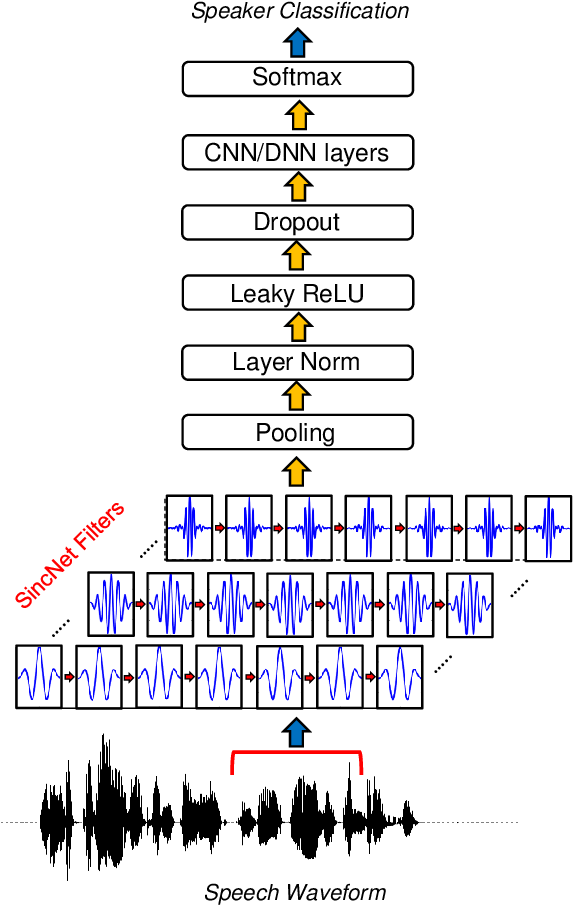
\includegraphics[width=120mm, keepaspectratio]{figures/sincnet-nn.png}
	\caption{SincNet architektúra~\cite{sincnet}.}
	\label{fig:sincnet-nn}
\end{figure}
\ \\
\newline
A SincNetet a TIMIT (462 beszélő) és Librispeech (2484 beszélő) adatbázisokkal tanították.
A beszédminták elejéről a szüneteket eltávolították, és LibriSpeech esetén azokat a mintákat, amelyek tartalmaztak legalább 125 ms hosszú szünetet, annak mentén feldarabolták. A TIMIT adatbázisnál egy beszélőtől 5 mintával tanítottak és 3 mintával teszteltek, míg LibriSpeechnél véletlenszerűen választott 12-16 másodperces mintákkal tanítottak és 2-6 másodpercesekkel teszteltek.
\newline
\begin{table}[!ht]
	\begin{tabular}{*3l} \toprule
		\bfseries Rendszer & \bfseries TIMIT & \bfseries LibriSpeech \\ \midrule
		DNN-MFCC & 0,99 & 2,02 \\
		\rowcolor{gray!10} 
		CNN-FBANK & 0,86 & 1,55 \\
		CNN-Raw  & 1,65 & 1,00 \\
		\rowcolor{gray!10} 
		SINCNET & 0,85 & 0,96 \\
		\bottomrule
		\hline
	\end{tabular}
	\centering
	\caption{Szöveg-független azonosítás eredményei adatbázisok szerint.}
	\label{fig:sincnet-identification}
\end{table}
\ \\
A \ref{fig:sincnet-identification}-es táblázat a CER (Classification Error Rate [\%]) hiba rátát mutatja. E szerint a SincNet jobban teljesít az MFCC, FBANK és nyers hullámformákkal tanított CNN-eknél mindkét adatbázis esetében, bár látható, hogy a sima CNN és a SincNet között minimális a különbség.
\newline
\begin{table}[!ht]
	\begin{tabular}{*3l} \toprule
		\bfseries Rendszer & \bfseries d-vector & \bfseries DNN-class \\ \midrule
		DNN-MFCC & 0,88 & 0,72 \\
		\rowcolor{gray!10} 
		CNN-FBANK & 0,60 & 0,37 \\
		CNN-Raw  & 0,58 & 0,36 \\
		\rowcolor{gray!10} 
		SINCNET & 0,51 & 0,32 \\
		\bottomrule
		\hline
	\end{tabular}
	\centering
	\caption{Szöveg-független ellenőrzés (verifikáció) eredményei.}
	\label{fig:sincnet-verification}
\end{table}
\ \\
\newline
A SincNettel nem jellemző vektorokat képeztek és a köztük lévő távolságot használták a hasonlóság mérésére, hanem osztályozással használják. Ebben az esetben zárt-halmazú beszélőazonosításról beszélünk. Ez sokkal kevésbé flexibilis, mert új beszélő esetén mindig újra kell tanítani a hálózatot, de cserébe jobb teljesítményre képes. A \ref{fig:sincnet-verification} ábrán egy d-vector nevű hangvektorokat képző neurális hálózatot hasonlítottak össze a SincNettel. Beszélőellenőrzés esetén a SincNet sokkal jobb EER-t ért el.
\newpage
\subsection{VoxCeleb2: Deep Speaker Recognition}

A VoxCeleb1 és VoxCeleb2 (2018) nagy méretű, beszélőfelismerés céljából készült adatbázisok. Az előbbi több mint 1000, utóbbi pedig több mint 6000 hangmintát tartalmaz hírességektől. Az adatbázisok felépítésének részleteit a \ref{voxceleb1} és \ref{voxceleb2} fejezetek ismertetik. Mindkét adatbázissal végeztek méréseket különböző neurális hálózatokkal, de a legjobb eredményeket illetve nyílt-halmazú beszélőfelismerést a VoxCeleb2-vel érték el~\cite{voxceleb2}.
\newline
\newline
Bemutatják a VGGVox nevű CNN alapú neurális hálózatot, amelyet spektrogramokkal tanítottak és hangvektorokat hoz létre. Előnye ennek a megoldásnak, hogy nyílt-halmazú beszélőfelismerésre használható, új beszélő esetén nem szükséges újra tanítani a hálózatot. 
\newline
\newline
Módosított VGG-M és ResNet architektúrákkal kísérleteztek. A modelleket contrastive loss veszteségfüggvénnyel tanították és előtanításra egy softmax réteget használtak keresztentrópiával, ami javította a modell teljesítményét. Tanító adathalmaznak a VoxCeleb2 adatbázist használták és a tesztelést a VoxCeleb1-el végezték. A méréseket EER és a \ref{eq:cdet} detektálási költség függvény szerint értékelték ki,

\begin{equation} \label{eq:cdet}
C_{det} = C_{miss} \cdot P_{miss} \cdot P_{target} + C_{fa} \cdot P_{fa} \cdot (1 - P_{target})
\end{equation}

ahol \emph{C\_miss} és \emph{C\_fa} alkalmazás specifikus paraméterek a hamis negatív és hamis pozitív hibák költsége, \emph{P\_miss} és \emph{P\_fa} pedig a hibák előfordulásának valószínűségét jelzik. \emph{P\_target} annak a valószínűsége, hogy a rendszer két olyan mintát hasonlít össze, amely egy embertől származik.
\newline
\begin{table}[!ht]
	\begin{tabular}{*4l} \toprule
		\bfseries Rendszer & \bfseries Tanítóhalmaz & \bfseries $C_{min}^{det}$ & \bfseries EER \\ \midrule
		I-vectors + PLDA & VoxCeleb1 & 0,73 & 8,8 \\
		VGG-M (Softmax) & VoxCeleb1 & 0,75 & 10,2 \\
		VGG-M & VoxCeleb1 & 0,71 & 7,8 \\
		VGG-M  & VoxCeleb2 & 0,609 & 5,94 \\
		ResNet-34 & VoxCeleb2 & 0,549 & 4,83 \\
		ResNet-50 & VoxCeleb2 & 0,429 & 3,95 \\
		\bottomrule
		\hline
	\end{tabular}
	\centering
	\caption{Beszélő ellenőrzés (verifikáció) eredményei.}
	\label{fig:sincnet-verification}
\end{table}

\newpage

\subsection{Utterance-level Aggregation for Speaker Recognition in the Wild}

A 2019-es cikk két fő témája egy olyan neurális hálózat létrehozása, amely képes különböző hosszúságú hangmintákból jellemző vektorokat képezni és olyan hangminták vizsgálata amelyek irreleváns zajokat is tartalmaznak~\cite{speaker_in_the_wild}.

\begin{figure}[!ht]
	\centering
	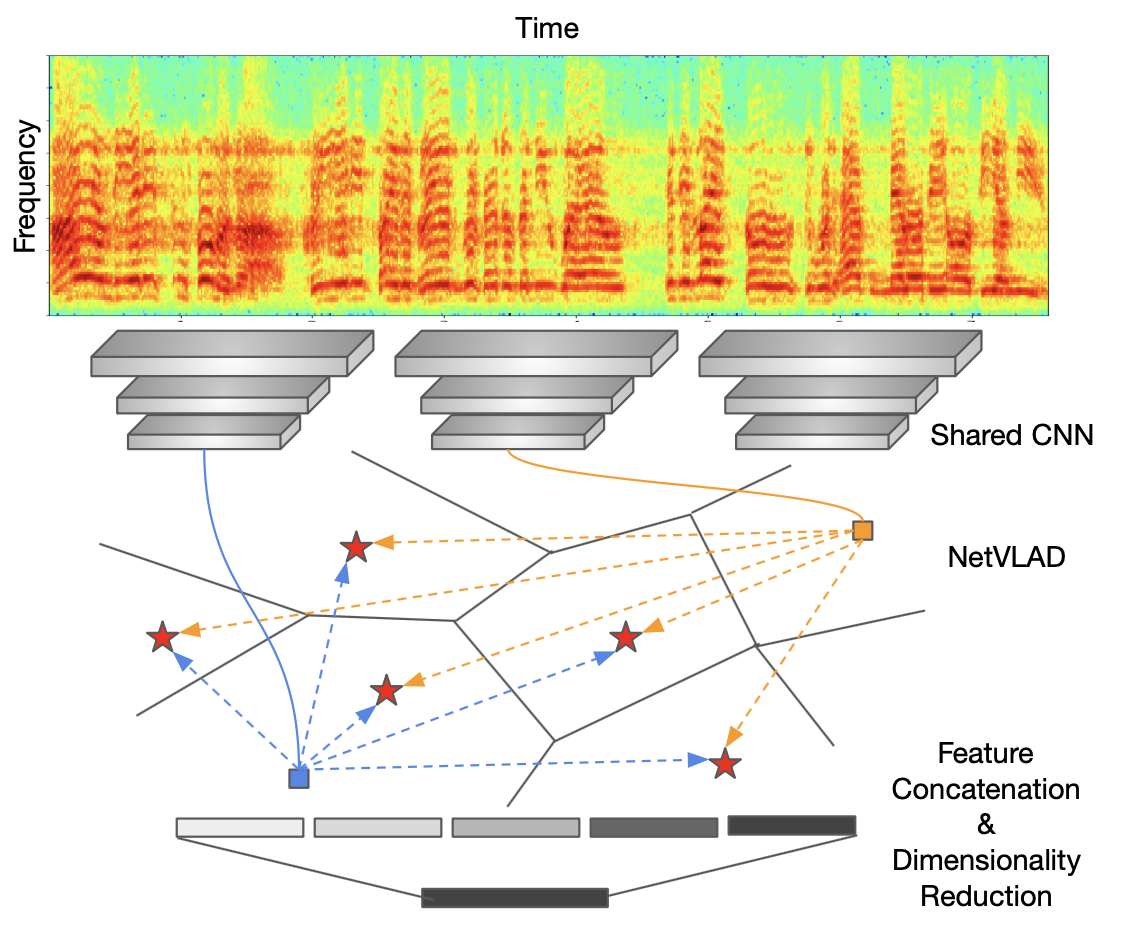
\includegraphics[width=150mm, keepaspectratio]{figures/frame-cnn.png}
	\caption{Neurális hálózat architektúra~\cite{speaker_in_the_wild}.}
	\label{fig:frame-cnn}
\end{figure}
\ \\
\newline
\newline
A hálózat három részből áll. Először egy módosított ResNet architektúrát használnak a keretszintű vektorok előállítására spektrogramokból. Az ábrán látható megosztott CNN-t hívjuk trönk hálózatnak. A keretszintű vektorok aggregálását a NetVLAD illetve GhostVLAD (Vector of Locally Aggregated Descriptors módszeren alapuló) hálózatokkal végzik. Legvégül egy FC (Fully Connected) réteget használnak a dimenzió 512-re csökkentésére.
\newline
\newline
A teljes modell end-to-end tanítására a VoxCeleb2 adatbázist használták és tesztelésként beszélőellenőrzést (verifikációt) mértek a VoxCeleb1-en.
\begin{figure}[!ht]
	\centering
	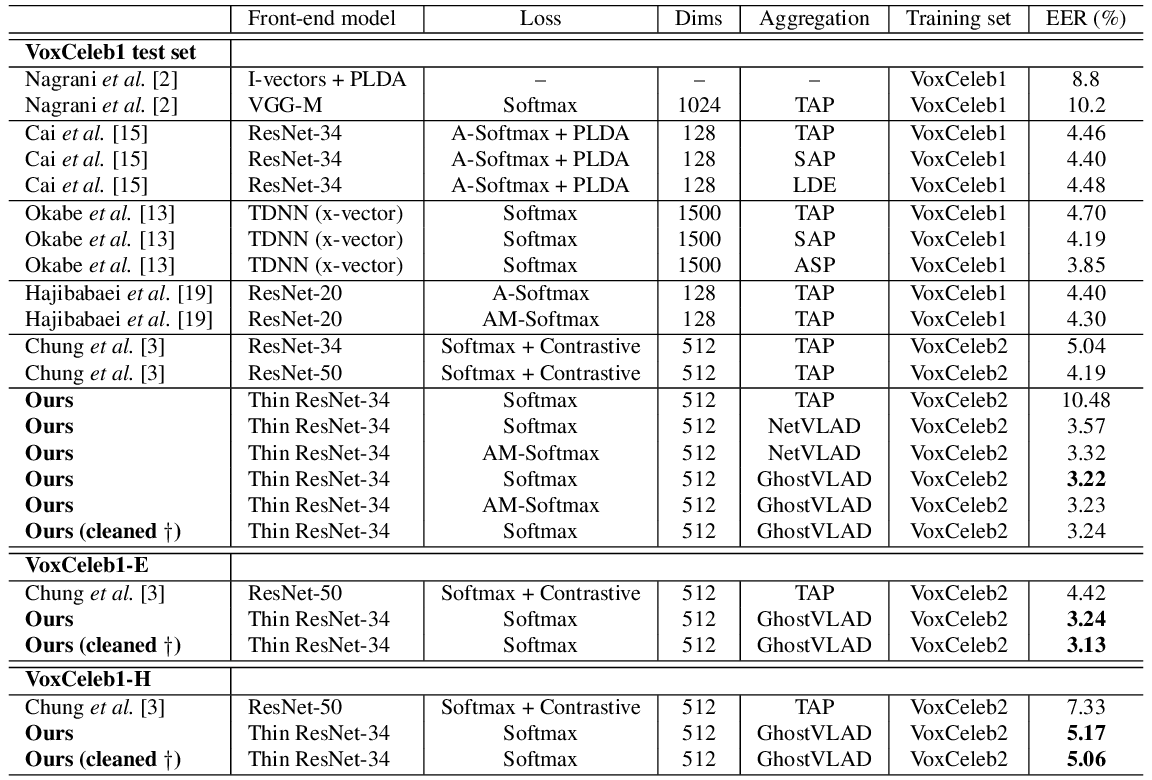
\includegraphics[width=150mm, keepaspectratio]{figures/frame-cnn-results.png}
	\caption{Neurális hálózat architektúra~\cite{speaker_in_the_wild}.}
	\label{fig:frame-cnn-results}
\end{figure}
\ \\
A \ref{fig:frame-cnn-results} táblázat mutatja a verifikációval mért EER-eket az akkori legkorszerűbb rendszerekkel szemben. Az addigiaknál lényegesen jobb EER-t értek el ezzel a módszerrel.

\section{A hangminták hossza}

Az eddigi rendszerekre hagyatkozva elmondható, hogy körülbelül 1-15 másodperces mintákkal tanították a neurális hálózatokat. Ez függ a beszédadatbázisban lévő hangminták méretétől, az előfeldolgozástól, és az határozza meg, hogy hiperparaméter optimizáció során mi bizonyul a legjobb értéknek. Ez rendszerenként változó. A \ref{section:modern_speaker_recognition} fejezetben ismertetett rendszerek és a voicemap kísérletek (\ref{section:voicemap_expermiments} fejezet) a következő eredményeket mutatták:

\begin{itemize}
	\item Deep speaker: 1-5 másodperces hangmintákból képzett 20-dimenziós MFCC-t használtak tanításhoz.
	\item LibriSpeech: 12-16 másodperces mintákkal tanítottak
	\item VoxCeleb2: 3 másodperces mintákból képzett spektrogrammokat használtak.
	\item Speaker Recognition in the Wild: Átlagosan 7-8 másodperces mintákat használnak (VoxCeleb2 adatbázis)
	\item voicemap: 3 másodperces minta volt a legjobb optimizálás után.
\end{itemize}

\section{Mérési környezet}

A mérésekhez a Google Colaboratoryt használtam, amely gépi tanulási kutatások és oktatás céljából felhő alapú környezetet biztosít. Hozzáférni Google fiókkal lehet, egy felhasználó egy virtuális gépet és egy Jupyter Notebookot kap. Választhatunk, hogy  a notebook a Python 2-es vagy 3-as verzióját támogassa, illetve, hogy CPU-n, GPU-n vagy TPU-n szeretnénk tanítani. A Tensor Processing Unit (TPU) a Google által fejlesztett gyorsító hardver egység Tensorflows tanításokhoz.
\newline
\newline
Az erőforrásokhoz fájlrendszert is kapunk. Ehhez hozzácsatolhatjuk a Google Drive fiókunkat, így elérhetjük a rajta tárolt adatokat. A notebookon keresztül elérjük a mögötte futó Linuxot is, lehet terminál parancsokat futtatni ha \emph{!} vagy \emph{\%} jelöléssel kezdjük a sort. Ez lehetővé teszi azt is, hogy pl. kisebb méretű dolgokat \emph{wget}tel töltsünk le vagy navigáljunk a fájlrendszerben, létrehozzunk új mappákat vagy töröljünk, áthelyezzünk fájlokat. Ugyan egyszerre több notebookot használhatunk, a fájlrendszer és a hardveres erőforrások ezek között megosztottak.

\subsection{Adatok előfeldolgozása}

Az előfeldolgozó szkript a TIMIT adatbázis esetében a hangmintákról eltávolítja a NIST Sphere fejlécet és a mondat előtti és utáni szüneteket. Ezután normalizálja a hangmintákat. A CMU Arctic esetében a hangminták alapból normalizálva vannak, ezért csak azonos méretűre kell vágni őket az egységes bemeneti dimenziók érdekében (ahogy a TIMIT esetében is).

\section{WaveNet classifier}

A \emph{WaveNet classifier} egy módosított WaveNet architektúra beszélőidentifikációhoz.

\subsection{WaveNet}

A WaveNet egy mély neurális hálózat audio hullámformák generálásához, amelyet a Google DeepMind publikált 2016-ban. Az ötletet az akkori felfedezések adták neurális autoregresszív generatív modellezés terén, amelyeket komplex eloszlások, például képek modellezésére használtak. Ezt felhasználva audio hullámformák generálásában új eredményeket értek el~\cite{wavenet}.

\begin{itemize}
	\item Képes olyan természetes hangzású beszéd hullámformák generálására, amit korábban parametrikus vagy konkatenatív beszédszintézissel sosem értek el. 
	\item Az audio hullámformák generáláshoz szükséges nagy receptív mezőt hatékonyan, nyújtott kauzális konvolúciókkal implementálja.
	\item Ha a modellt a beszélők identitásával tanítják, képes új hangok generálására.
	\item A zene generálás és a beszédfelismerés terén is ígéretesnek bizonyult.
\end{itemize}

\subsubsection{Nyújtott kauzális konvolúció}

A modell autoregresszív, vagyis a kimenete korábbi időpillanatokban felvett értékeitől függ. Ez azért fontos, mert a WaveNet egy generatív modell. A generált hullámforma \emph{t}-edik időpillanatbeli értéke nem függhet jövőbeli értékektől. A kauzalitás legegyszerűbb implementációja ha legalább \emph{kernel-1} méretű paddinget adunk a konvolúcióhoz.

\begin{figure}[!ht]
	\centering
	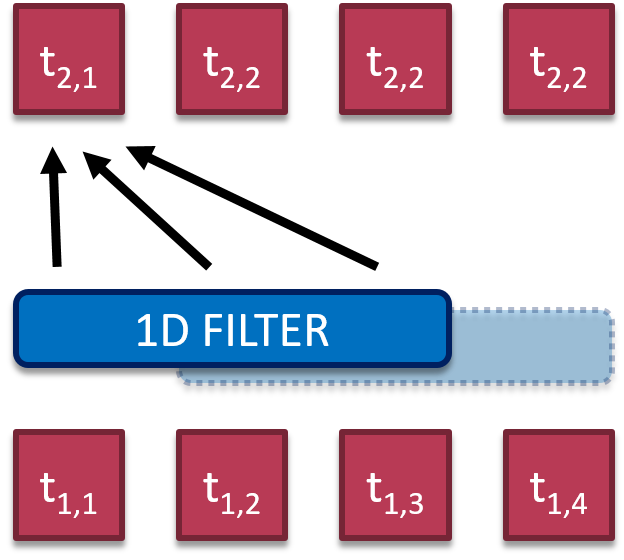
\includegraphics[width=80mm, keepaspectratio]{figures/1d-conv.png}
	\caption{1D nem kauzális konvolúció.}
	\label{fig:1d_noncausal_conv}
\end{figure}

\begin{figure}[!ht]
	\centering
	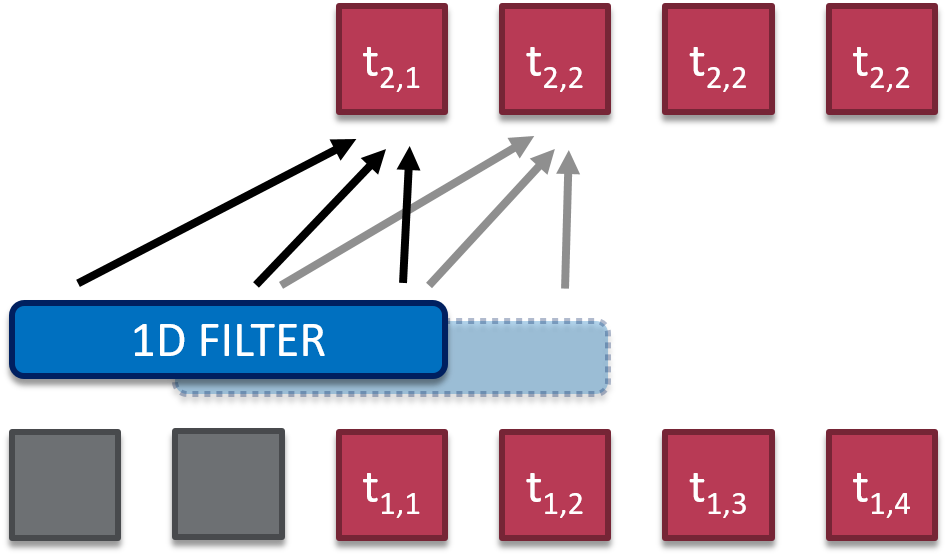
\includegraphics[width=120mm, keepaspectratio]{figures/1d-causal-conv.png}
	\caption{1D kauzális konvolúció paddinggel.}
	\label{fig:1d_causal_conv}
\end{figure}

\newpage

A \ref{fig:1d_noncausal_conv} ábra egy nem kauzális 1D konvolúciót mutat. A $t_{i, j}$ az i-edik rétegbeli j-edik neuron. Látható, hogy a $t_{2,1}$ jövőbeli időpillanatokból kap értékeket a szűrőn keresztül. Ennek megoldása a szűrő eltolása padding segítségével. Ezt szemlélteti a \ref{fig:1d_causal_conv} ábra, ahol az egyes neuronok csak korábbi időpillanatokból kapnak értékeket. 
\newline
\newline
A beszéd generálásánál a \emph{t}-edik időpillanatban a hullámforma értéke a korábbi adatoktól függ. Ahhoz, hogy magas frekvenciájú, pl. 16 kHz frekvencián mintavételezett 
hangadattal tanítsuk a hálózatot nagy receptív mezőre van szükség. A receptív mező az a szélesség, amit a szűrő lát a bemenetből. 16 kHz esetén egy másodpercnyi jelet 16000 szám reprezentál. Ahhoz, hogy a hálózat helyesen jósolja meg a következő generált értéket, a hosszú távú dependenciákat figyelembe kell vennie, tehát a receptív mező méretét elég nagyra kell megválasztani. A probléma ekkora mezők esetén, hogy sok konvolúciós réteget igényelnek (egy korábbi időpillanatbeli adat plusz egy konvolúciós réteget igényel), ami növeli a számítási komplexitást.
\newline
\newline
A nyújtott konvolúciók erre adnak hatékony megoldást. A filter meghatározott távolságokkal kihagy valamennyi inputot, majd figyelembe vesz egyet. Egymás utáni rétegekben a nyújtási tényezőt exponenciálisan növelve a receptív mező is exponenciálisan fog nőni.

\begin{figure}[!ht]
	\centering
	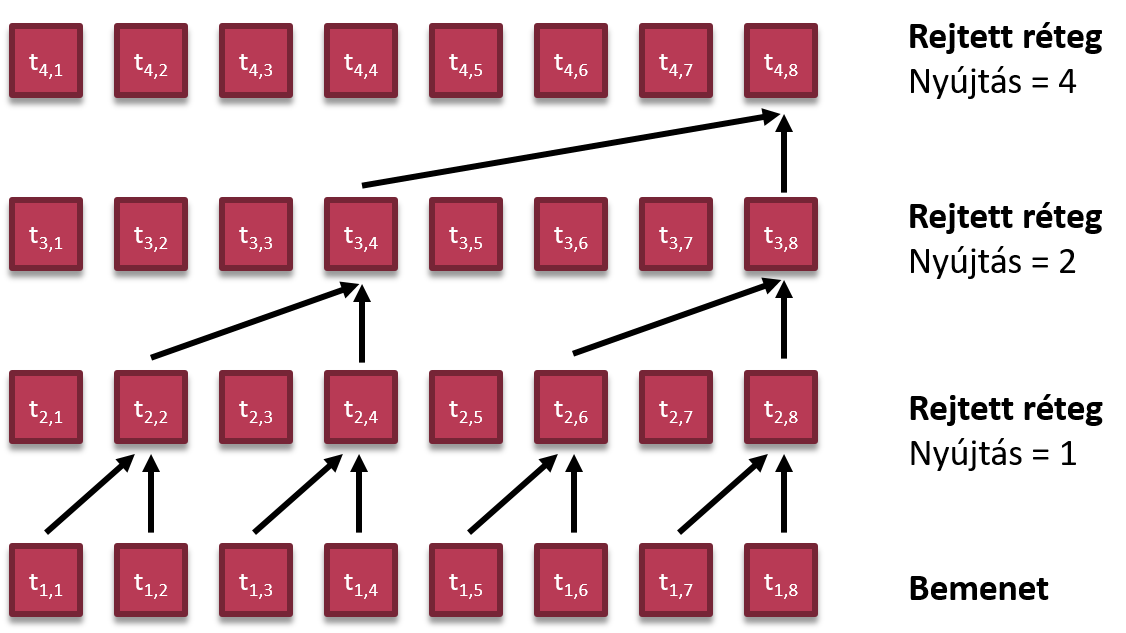
\includegraphics[width=150mm, keepaspectratio]{figures/1d-dilated-conv.png}
	\caption{1D nyújtott kauzális konvolúciós rétegek.}
	\label{fig:1d_dilated_conv}
\end{figure}

\subsubsection{SoftMax eloszlás}
A WaveNet SoftMax réteget használ a $p(x_t|x_1,\dots,x_t)$ feltételes valószínűségi eloszlás modellezésére.
Az audio jeleket általában 16 bites egészekkel kódolják, amelyek 65536 értéket vehetnek fel. Ebben az esetben a SoftMax rétegnek 65536 valószínűséget kell kimenetként adnia, melyek összege 1. A $\mu$-law kvantálást alkalmazva a beszédjel 256 biten kódolható és később az inverz transzformációval jó minőségben visszaállítható.
\newline
\newline
Az emberi hallás sokkal érzékenyebb alacsony amplitúdójú hangok kvantálási zajára, mint a magasabbakéra. Erre alapozva a $mu$-law kvantáló a jelet egy logaritmikus függvénnyel kvantálja úgy, hogy az alacsonyabb amplitúdójú jelek nagyobb felbontással (több bittel), a magasabbak pedig kisebbel lesznek kódolva. Ez növeli a SoftMax réteg hatékonyságát is, mert nagyobbak lesznek a valószínűségek közötti különbségek.
\newline
\newline
A tanítást a WaveNet klasszifikációs problémaként kezeli. A bemeneteket OneHot kódolással adjuk meg, a SoftMax réteg pedig az így kódolt egészekre ad valószínűségi eloszlást.

\subsubsection{Reziduális blokkok}

A WaveNet architektúra egymáshoz csatolt reziduális blokkokból és ún. kapcsolat-ugrásokból (skip-connection) épül föl. A reziduális hálózatok előnye, hogy orvosolják az elenyésző gradiens problémát, így sokkal mélyebb hálózat építhető.

\begin{figure}[!ht]
	\centering
	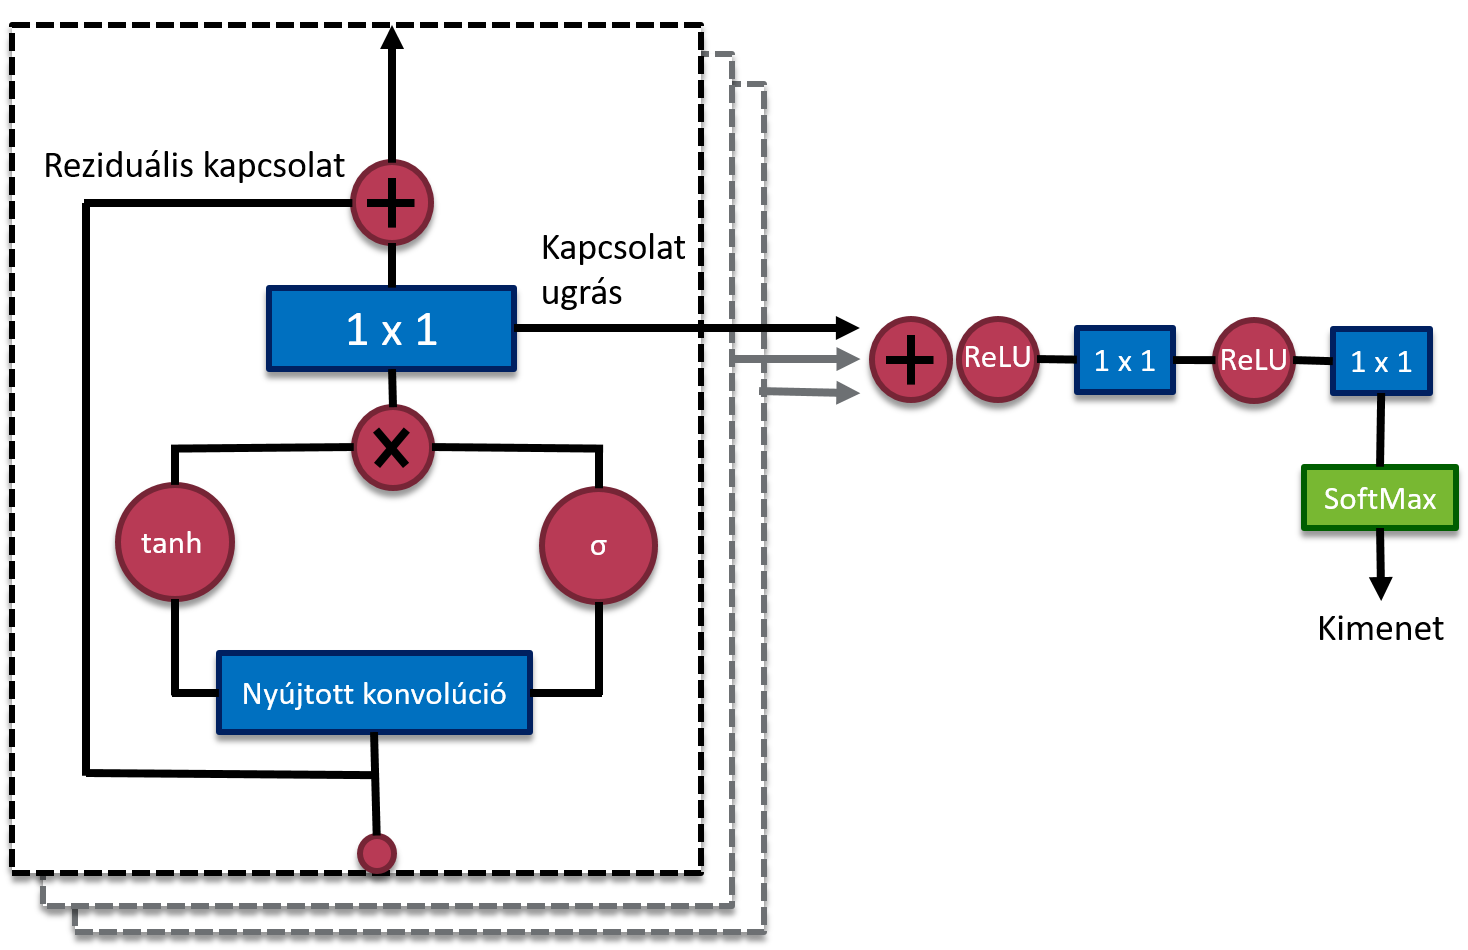
\includegraphics[width=150mm, keepaspectratio]{figures/wavenet_arch.png}
	\caption{WaveNet architektúra.}
	\label{fig:wavenet_arch}
\end{figure}

Egy reziduális blokk bemenete egy 2x1-es konvolúciós rétegen megy keresztül. Balra egy \emph{tanh}, jobbra egy szigmoid aktivációs függvényen haladnak át, majd elemenkénti szorzás és 1x1 konvolúció után egyrészt átugorja a reziduális kapcsolatot, illetve azzal együtt bemenetként szolgál a következő reziduális egységnek. Az 1x1 konvolúciós rétegek a dimenzionalitás változtatására szolgál. Külön 1x1 konvolúciós szűrők skálázzák a kimenetet a következő reziduális blokk bemenetére, és a kapcsolat-ugrásokhoz.

\subsection{Módosított WaveNet architektúra}

A módosított WaveNet architektúra segítségével a WaveNetet beszélőfelismerésre használhatjuk.
\bigskip
\begin{python}
	from WaveNetClassifier import WaveNetClassifier
	
	wnc = WaveNetClassifier((96000,), (10,), kernel_size = 2, dilation_depth = 9,
	                         n_filters = 40, task = 'classification')
	
	wnc.fit(X_train, y_train, validation_data = (X_val, y_val), epochs = 100,
	        batch_size = 32, optimizer='adam', save=True, save_dir='./')
	
	y_pred = wnc.predict(X_test)
	
\end{python}
\bigskip
A WaveNetClassifier objektum paraméterei:

\begin{itemize}
	\item \emph{input\_shape}: Bemeneti dimenziók tuple formájában. Például ha a bemenet egy 6 s hosszú hullámforma 16 kHz-en mintavételezve, a bemeneti dimenziók (96000,)
	\item \emph{output\_shape}: Kimeneti dimenziók tuple formájában. Például ha 100 osztály szerint klasszifikálunk, a kimeneti dimenziókból képzett tuple (100,).
	\item \emph{kernel\_size}: A konvolúciós filter/kernel mérete a reziduális blokkokban.
	\item \emph{dilation\_depth}: A reziduális blokkok száma.
	\item \emph{n\_filters}: A konvolúciós filterek száma a reziduális blokkokban.
	\item \emph{task}: Klasszifikáció vagy regresszió.
	\item \emph{regression\_range}: A regresszió céltartománya lista vagy tuple formátumban.
	\item \emph{load}: Előző WaveNetClassifier betöltése (bool).
	\item \emph{load\_dir}: A betölteni kívánt modell könyvtára.
\end{itemize}

\subsection{Eredmények}

A WaveNet classifiert TIMIT és CMU Arctic beszédadatbázisokkal teszteltem. A TIMIT beszédkorpusszal csak kevés beszélő esetén ért el jó eredményt, több mint 20 beszélő esetén a modell nem tanult. Ennek valószínűsített oka, hogy a TIMIT adatbázis beszélőnként 10 hangmintát tartalmaz.

\setlength\arrayrulewidth{0.6pt}

\begin{table}[!ht]
	\begin{tabular}{l|l} \toprule
		\bfseries Beszélők száma & 18 \\
		\rowcolor{gray!10}
		\bfseries Minta/beszélő & 100\\
		\bfseries Minta össz. & 1800 \\
		\rowcolor{gray!10}
		\bfseries Minta hossza & 4000 \\
		\bfseries Epochok száma & 43\\
		\rowcolor{gray!10}
		\bfseries Hiba & 0.0013 \\ 
		\bfseries Pontosság & 1.0 \\ 
		\bottomrule
		\hline
	\end{tabular}
	\centering
	\caption{Paraméterek CMU Arctic adatbázissal.}
	\label{fig:wavenet-arctic}
\end{table}
\ \\
A TIMIT TRAIN 630 beszélőt tartalmaz hangmintákat. Először lefuttattam rajta egy módosított előfeldolgozó szkriptet (LibriSpeech respository része), ami levágja a szüneteket a hangminták elejéről és végéről a WRD fájlnak megfelelően, majd normalizálja az amplitúdókat. ezekből kiválogattam azokat, amelyek legalább 2,5 mp hosszúak voltak, és beszélőnként 2:1 arányban tanító és teszthalmazra daraboltam őket.
Kevés, 10 beszélővel és 2,5 másodperces hangmintákkal tanítva, a teszt adathalmazon a hálózat 96.799 \%-os pontosságot ért el.
\newline
\newline
A CMU Arctic adatbázisokat letöltöttem a Google Colaboratory-s fájlrendszerre és egy mappa alá mozgattam őket. Ehhez csak az adatbázis kódjára volt szükség, mindegyik azonos kezdetű url-en található.
A CMU Arctic 16 bit-es wav fájlokat tartalmaz. Normalizálásként minden mintavételezett értéket leosztottam a maximális hosszal ($2^15 + 1$), hogy 0 és 1 közötti értéket vegyenek fel.
\newline
\newline
Tanítómintáknak 2-3 másodperces részeket választottam. A megfelelő hosszú wav fájlokból kivágtam a [0:40000] részt, így pontosan $40000/16000 = 2,5$ s-os szeleteket kaptam. Mind a 18 adatbázisból kiválasztottam 100 ilyen mintát. Ezeket véletlenszerűen összekevertem és ez az 1800 elemű halmazzal tanítottam. Az epochok száma 200 volt, de mivel a tanítás a 43-44. epochnál már 1-es pontosságot és közel 0 veszteséget mutatott, leállítottam a folyamatot. 
\newline
\newline
\begin{figure}[!ht]
	\centering
	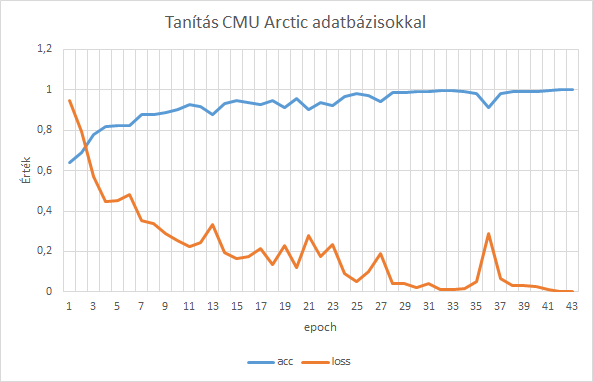
\includegraphics[width=150mm, keepaspectratio]{figures/wavenet-train-cmu-arctic.png}
	\caption{WaveNet tanítása CMU Arctic adatbázisokkal.}
	\label{fig:wavenet-train-cmu-arctic}
\end{figure}
A teszthalmazba a tanítómintákon kívüli minimum 40000 hosszú wav fájlok kerültek, összesen 10152 minta.
Az elvárt kimeneteket one-hot kódoltam és kiértékeltem a modellt a tesztadatokon. A felismerés pontossága $97,3$ \% volt 18 ember esetén.

\section{Voicemap}

A \emph{voicemap} egy nyílt forráskódú deep learning projekt beszélőfelismerő feladatok elvégzéséhez. A GitHub repository tartalmazza a modell kódját, a tanítást, különböző kísérleteket és egy hiperparaméter-optimizált, előre tanított modellt. Az implementációhoz \emph{Kerast} illetve újabb verziókban \emph{Pytorchot} használ~\cite{voicemap_github}.
\newline
\newline
A projekt célja, hogy későbbiekben egy olyan általános, pip által telepíthető csomag legyen, ami könnyen felhasználható beszélőfelismeréssel kapcsolatos feladatok elvégzésére.

\subsection{A projekt általános felépítése}

Mivel a saját alkalmazásomban felhasználtam és átalakítottam a projekt egyes részeit,
röviden bemutatom a felépítését.

\begin{itemize}
	\item \emph{models.py}: A konvolúciós enkóder létrehozását és a sziámi hálózat építését végzi el.
	\item \emph{librispeech.py}: Keras szekvencia osztály Librispeech beszédadatbázisból származó hangminták tárolására, előfeldolgozására és generálására tanításhoz. Fő paraméterei a következők:
	\begin{itemize}
		\item \emph{subsets}: Mely LibriSpeech adathalmazokat tartalmazza.
		\item \emph{seconds}: Az ennél rövidebb időtartamú hangmintákat figyelmen kívül hagyja.
		\item \emph{stochastic}: Sztochasztikus módban a mintákból véletlenszerűen vágjuk ki a \emph{seconds} hosszúságú darabot.
		\item \emph{pad}: Padding esetén a rövidebb hangmintákat nullával feltöltve a megadott méretre alakíthatjuk. Sztochasztikus mód esetén véletlenszerűen oszlik el a hangminta előtti és utáni nullák száma.
	\end{itemize}
	
	A két legfontosabb függvénye:
	
	\begin{itemize}
		\item \emph{build\_verification\_batch}: A sziámi hálózat teszteléséhez generál olyan batchet, amelyben az ugyanattól és az eltérő beszélőktől származó hangmintapárok száma azonos (50\%-50\%). A batch egy eleme két hangmintából és egy címkéből áll, ami jelzi, hogy egyazon vagy más-más beszélőktől származnak.
		\item \emph{build\_n\_shot\_task(k, n)}: Visszaad egy segédhalmazt $n$ mintával minden egyes $k$ beszélőhöz és visszaad egy mintát, amiről a modellnek el kell döntenie, hogy melyik beszélőhöz tartozik.
	\end{itemize}
	\item \emph{utils.py}: Fő feladata az adatok preprocesszálása és az \emph{n\_shot\_task\_evaluation} függvény által az \emph{n-shot k-way} feladat kiértékelése. A few-shot kiértékeléshez alábbi argumentumokat adhatjuk meg:
	
	\begin{itemize}
		\item  \emph{model}: A tesztelendő modell.
		\item  \emph{dataset}: A tesztmintákat tartalmazó adathalmaz objektum.
		\item  \emph{preprocessor}: Előfeldolgozó függvény a minták csökkentett mintavételezésére és standardizálására.
		\item  \emph{num\_task}: A feladatok száma.
		\item  \emph{n}: Hány hangminta tartozik egy beszélőhöz a segédhalmazban.
		\item  \emph{k}: Ennyi beszélő, azaz osztály van a segédhalmazban.
		\item  \emph{network\_type}: Sziámi vagy klasszifikációs.
		\item  \emph{distance\_metric}: Sziámi hálózat esetén a hangvektorok közötti távolságmetrika.
	\end{itemize}
\end{itemize}

\subsection{Az implementált modellek}

A projekt két modellt vizsgál; egy sziámi neurális hálózatot (a konvolúciós sziámi hálózat részletes leírása a \ref{section:siamese_conv} fejezetben található) és egy sima konvolúciósat klasszifikációval. Mindkét hálózat alapja alapja egy konvolúciós enkóder, amely a nyers hangmintákból kinyeri a jellemzőket és hangvektorokat állít elő belőlük. Az enkóder hálózat a több egymást követő konvolúciós blokk áll. Egy konvolúciós blokk felépítése a \ref{fig:conv_encoder_block} ábrán látható. Ezek egy konvolúciós rétegből és regularizációs
rétegekből tevődnek össze.

\begin{figure}[!ht]
	\centering
	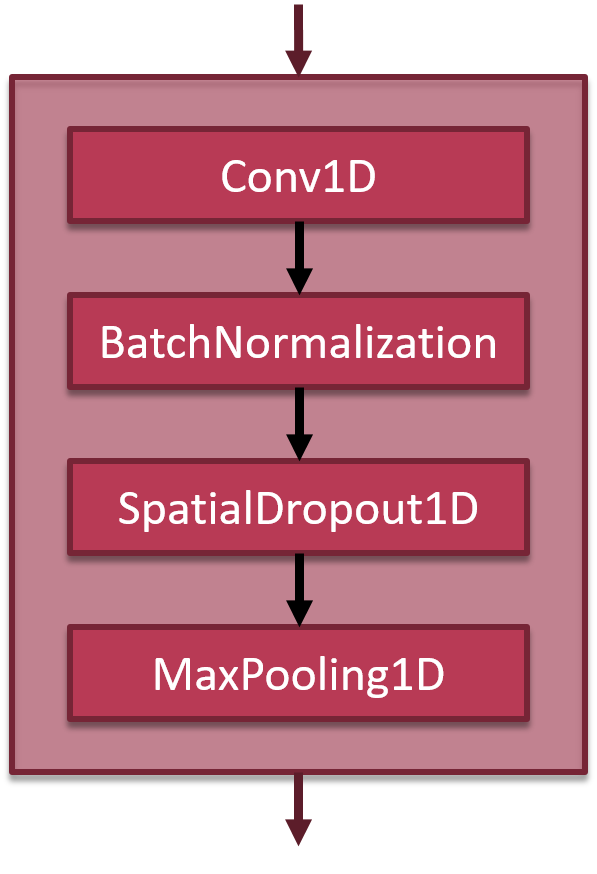
\includegraphics[width=80mm, keepaspectratio]{figures/conv_encoder_block.png}
	\caption{Egy konvolúciós enkóder blokk felépítése.}
	\label{fig:conv_encoder_block}
\end{figure}

\begin{itemize}
	\item Conv1D: 32-es méretű filterekkel, ahol a filterek száma arányosan nő azzal, hogy a blokk hányadik a sorban. Az aktivációs függvény \emph{ReLu}.
	\item BatchNormalization: Batchenként normalizálja az előző réteg kimeneteit úgy, hogy az átlag 0-hoz, a szórás 1-hez közelítsen. Regularizációra használják.
	\item SpatialDropout1D: Sima dropout réteg esetén az egyes neuronokat valamekkora valószínűséggel figyelmen kívül hagyjuk. Például egy [[1, 2, 3], [2, 3, 1]] tömbnek a kimenete sima dropout esetén lehet [[1, 0, 3], [0, 3, 1]], itt teljesen függetlenek egymástól a kinullázások. Spatial dropout esetén az adott dimenzió mentén mindent kinullázunk. Például [[1, 0, 3], [2, 0, 1]]. Regularizációra használják.
\end{itemize}
\ \\
Négy ilyen konvolúciós blokk követi egymást, majd további regularizáció: egy \emph{GlobalMaxPool1D} és egy \emph{Dense} réteg a hangvektor méretével.

\begin{figure}[!ht]
	\centering
	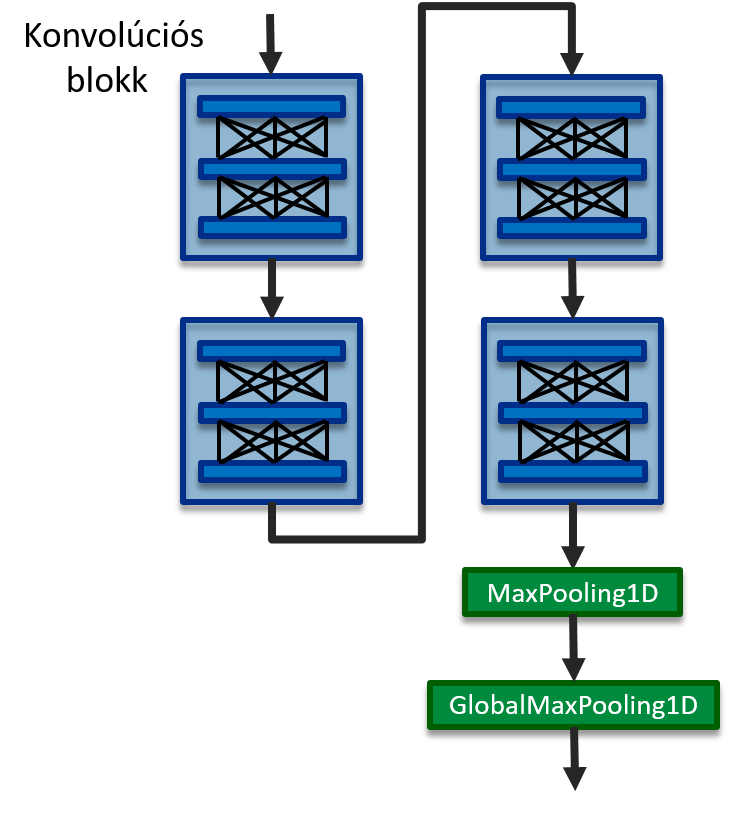
\includegraphics[width=100mm, keepaspectratio]{figures/conv_encoder.png}
	\caption{A konvolóciós enkóder felépítése.}
	\label{fig:conv_encoder}
\end{figure}
\ \\
A sziámi hálózat alapja két enkóder hálózat, amelynek súlyai megosztottak, tehát úgy is tekinthetünk rá, hogy egy enkóder hálózatra két bemenetet adhatunk. A hangminták a hálózaton áthaladva jellemző vektorokká alakulnak. Ezt a részt a konvolúciós enkóder végzi. Ezután a két vektor közötti távolságmetrikát a sziámi hálózat kiszámolja. Ezen távolság alapján számolja ki a veszteséget és javítja a súlyokat.
\ \\
Az implementált távolságmetrikák a következők:

\begin{itemize}
	\item \emph{weighted\_l1}: Az eredeti one-shot cikk szerinti távolságmetrika. $v_1$ és $v_2$ vektorokra $\sqrt{v_1-v_2}$.
	\item \emph{uniform\_euclidean}: Euklideszi távolság két vektor között.
	\item \emph{cosine\_distance}: Koszinusz távolság, azaz a két vektor által bezárt szög koszinuszát méri.
\end{itemize}

A kiszámolt távolság ezután minden esetben áthalad egy szigmoid aktivációs függvényű \emph{Dense} rétegen, ami $0$ és $1$ közé nyomja az eredményt.

\subsection{Beszédadatbázisok és generátorok}

A voicemap tanításhoz és teszteléshez a \emph{LibriSpeech} adatbázis \emph{dev-clean}, \emph{train-clean-100} és \emph{train-clean-360} adathalmazokat használja, amelyek sorban $40$, $251$ és $921$ különböző beszélőtől tartalmaznak nyers hangfájlokat.
\newline
\newline
Egy adathalmazt egy adatgenerátor osztály reprezentál ami a keras.util.Sequence osztályból származik. Az adatgenerátorok nagy adathalmazok esetén hasznosak, amikor az egész adathalmaz nem fér bele a memóriába. Ilyen esetekben egyesével generálnak adatokat.
\newline
\newline
A \emph{keras.util.Sequence} osztályból való leszármaztatás miatt az adatgenerátorban implementálni kell a \emph{\_\_len\_\_} és \emph{\_\_get\_item\_\_} függvényeket. Előbbi az adathalmaz méretét adja vissza, utóbbi annak indexelését teszi lehetővé. Továbbá biztosítja, hogy egy epochon belül egy mintával csak egyszer tanítjuk a modellt.

\subsection{Tanítás}

A sziámi és a sima klasszifikációs hálózat nagyrészt közös paraméterekkel rendelkeznek. A fő különbség, hogy míg a sziámi veszteségfüggvénye bináris keresztentrópia, és a veszteség az alapján dől el, hogy a hangminta pár egyazon vagy más beszélőktől származik, a klasszifikációs hálózat kategórikus keresztentrópiát használ, tehát a hangmintát megpróbálja besorolni $k$ osztály valamelyikébe $k$ beszélő esetén. A közös paraméterek:

\begin{itemize}
	\item hangminta hossza: 3 sec
	\item batchsize: 64
	\item filterek száma: 128
	\item jellemző vektor dimenzió: 64
	\item dropout: 0
	\item steps\_per\_epoch: 500
	\item kiértékelési feladatok száma: 500
	\item n\_shot\_klasszifikáció: 1
	\item k\_way\_klasszifikáció: 5
\end{itemize}

Tehát mindkét modell optimizált hiperparamétereket használ, \emph{Adam} optimizálót és veszteségfüggvényként keresztentrópiát. Egy epoch $500$ batch iterációból áll és egy batch méret $64$.
Az epochok végén három callback fut le.
\newline
\newline
Minden epoch végén kiértékelés történik: 500 \emph{1-shot 5-way} feladat átlagos eredménye jelzi a pontosságot. Amennyiben ez növekszik a modellről \emph{checkpoint} készül (\emph{ModelCheckpoint}).
Továbbá ha a kiértékelés során a pontosság nem nő, a \emph{ReduceLROnPlateau} csökkenti a tanulási rátát.


\subsection{Kísérletek és optimalizálás} \label{section:voicemap_expermiments}

A repositoryban számos kísérlet található a legjobb teljesítmény elérésére. A \emph{wide\_vs\_tall} szkript leméri, hogy a modell hogyan teljesít különböző hosszúságú hangmintákkal tanítva. A mérés alatt \emph{1-shot 5-way} feladatokkal, azaz 5 különböző beszélőtől 1-1 beszédmintával validálta a modellt~\cite{voicemap_medium}.

\begin{figure}[!ht]
	\centering
	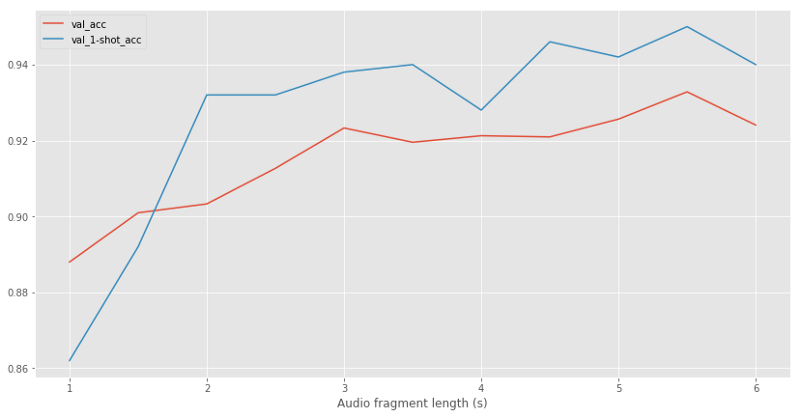
\includegraphics[width=150mm, keepaspectratio]{figures/voicemap-wide-vs-tall.png}
	\caption{Voicemap: Regisztrációs fázis.}
	\label{fig:voicemap-wide-vs-tall}
\end{figure}

A \ref{fig:voicemap-wide-vs-tall} ábrán látható, hogy a hangminta méretét növelve a modell valóban jobban tanul, de a több adat miatt megnövekedik a tanítási idő és több memóriára van szükség. A grafikon mutatja, hogy 3 másodperc után a validáció stagnálni kezd, ezért az erőforrásokat és a tanítási időt figyelembe véve ez tűnik a legjobb választásnak.
\newline
\newline
A \emph{grid\_search\_siamese\_network} szkript hiperparaméter optimizációt végez a sziámi hálózaton a filterek számát, a hangmintákból képzett vektorok hosszát és a dropoutot vizsgálva. A talált legjobb paraméterek:

\begin{itemize}
	\item filterek száma: 128
	\item jellemző vektor dimenzió: 64
	\item dropout: nincs
\end{itemize}
\ \\
A \emph{k\_way\_accuracy} kísérlet a hiperparaméter optimalizált modell teljesítményét méri le különböző \emph{n-shot k-way} feladatokkal. A pontosságot a \ref{fig:voicemap-n-shot-k-way} ábra mutatja.

\begin{figure}[!ht]
	\centering
	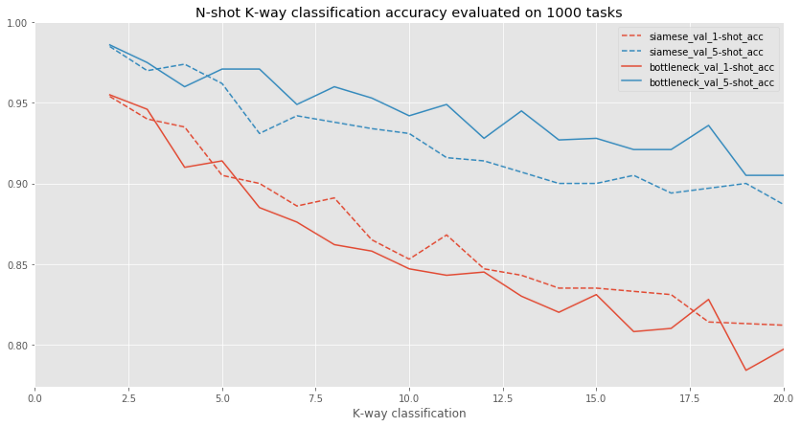
\includegraphics[width=150mm, keepaspectratio]{figures/voicemap-n-shot-k-way.png}
	\caption{Voicemap: n-shot k-way pontosság.}
	\label{fig:voicemap-n-shot-k-way}
\end{figure}
\ \\
\emph{1-shot k-way} feladatok esetén a sziámi hálózat átlagosan jobban teljesít sima klasszifikációsnál, de \emph{5-shot k-way} feladatok esetén már az utóbbi kerül fölénybe. Ez valószínűleg annak köszönhető, hogy 5 hangminta - beszélő párból a sima osztályozó hálózat már jobban meg tudta tanulni a beszélőket a sziáminál.


\begin{figure}[!ht]
	\centering
	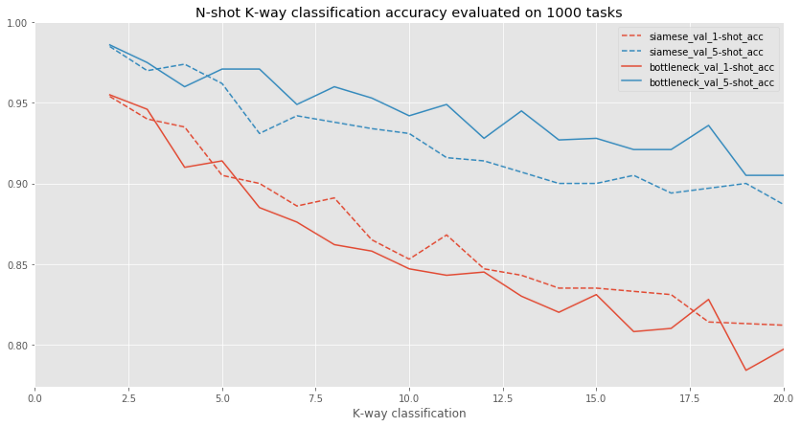
\includegraphics[width=150mm, keepaspectratio]{figures/voicemap-n-shot-k-way.png}
	\caption{Voicemap: n-shot k-way pontosság.}
	\label{fig:voicemap-n-shot-k-way}
\end{figure}

\newpage
\ \\
Lemértem sziámi hálózat esetén a contrastive loss és bináris keresztentrópia veszteségfüggvények közötti különbséget. Mindkét modellt az optimizált hiperparaméterekkel 50 epochon keresztül tanítottam.

\begin{figure}[!ht]
	\centering
	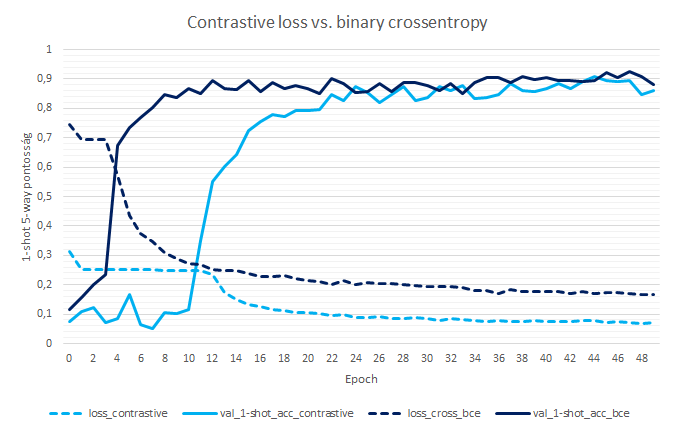
\includegraphics[width=150mm, keepaspectratio]{figures/contrastive_vs_bce.png}
	\caption{Voicemap: n-shot k-way pontosság.}
	\label{fig:contrastive_vs_bce}
\end{figure}
\ \\
A \ref{fig:contrastive_vs_bce} grafikon mutatja, hogy a \emph{1-shot 5-way} pontosság a 20. epochnál kezd 90\% fele konvergálni. A maximális pontosság contrastive lossnál a 44. epochnál 90,8\%, míg bináris keresztentrópia esetén a 47. epochnál 92,6\%.

\newpage

\subsection{Saját kísérlet: Triplet loss}


A sziámi hálózatoknak egy ismert költségfüggvénye a \emph{triplet loss} függvény. Ezt a \emph{gradient descent} módszerrel optimizálva tanítjuk a hálózatot. A triplet loss három bemenetet igényel, amelyek jelen példában a hangokból képzett jellemző vektorok. Az egyik egy rögzített hang vektora, ez az ún. \emph{anchor}. A másik kettő pedig egy pozitív és egy negatív minta. A pozitív ugyanattól a beszéltőtől származik mint az \emph{anchor} vektor, a másik különbözőtől~\cite{triplet_semi_hard}.
\begin{equation}\label{eq:4}
\mathcal{L}_{triplet}(A, P, N) = \max(d(A, P) - d(A, N) + m, 0)
\end{equation}
\ \\
A $d$ a távolságfüggvény, ami lehet például euklideszi távolság. A \emph{triplet loss} veszi az anchor és a pozitív meg az anchor és a negatív minta távolságainak különbségét, majd ezt eltolja az $m$ küszöbértékkel. Ha az előbbi pozitív ezt veszi eredményül, egyébként nullát.

\begin{figure}[!ht]
	\centering
	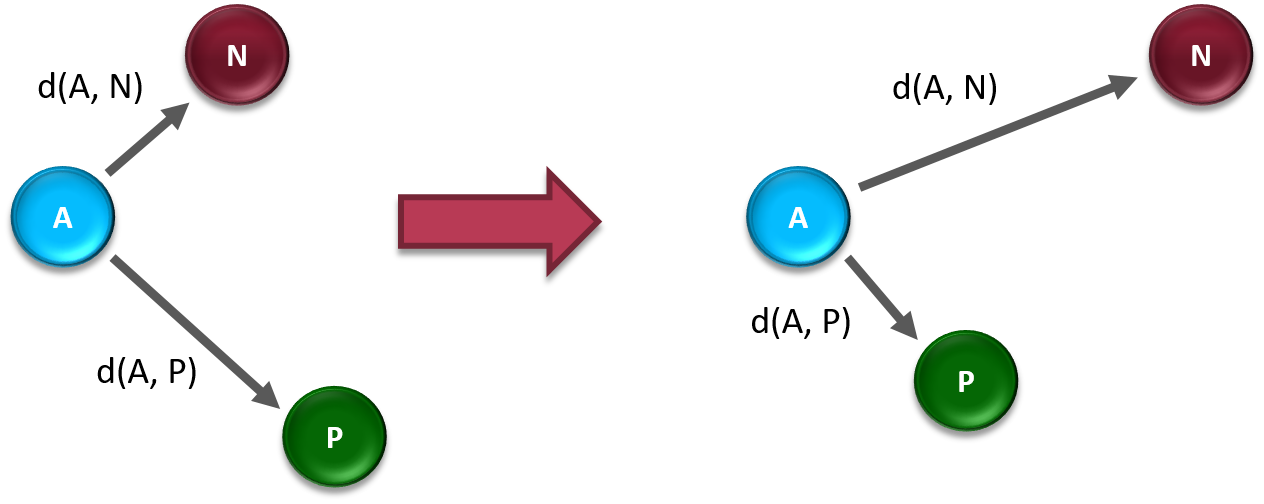
\includegraphics[width=100mm, keepaspectratio]{figures/triplet-loss.png}
	\caption{A triplet loss függvény csökkenti a távolságot a hasonló és növeli a különböző minták között.}
	\label{fig:triplet-loss}
\end{figure}
\ \\
Akkor jó a vektorok elhelyezkedése a metrikus térben, ha a hasonlók között a távolság kicsi, a különbözők között pedig nagy. Azt szeretnénk elérni, hogy
$d(A, P) \le d(A, N)$ fenn álljon. Átrendezve a $d(A, P) - d(A, N) \le 0$ egyenletet kapjuk. Ezt kielégíti a $d(A, P) = 0$, $d(A, N) = 0$ megoldás. A másik triviális megoldás, ha a pozitív és negatív minta kódolása ugyanaz lenne, ekkor ugyanis $d(A, P) = d(A, N)$ így $d(A, P) - d(A, N) = 0$. Szeretnénk, ha a neurális hálózat nem nullvektorokkal vagy azonos vektorokkal kódolná az összes képet, ezért hozzáadunk egy $m$ küszöbértéket az egyenlethez.

\begin{equation}\label{eq:5}
\begin{aligned}
d(A, P) + m \le d(A, N) \\
d(A, P) - d(A, N) + m \le 0
\end{aligned}
\end{equation}
\ \\
Ideális esetben a $d(A, P) - d(A, N) + m$ negatív, ilyenkor a veszteség 0. Ha nem így van, a triplet loss ezt a veszteséget adja vissza. A költségfüggvény a tanítóhalmazban lévő tripletekre alkalmazott triplet lossok összege. Ezt minimalizálva a \ref{fig:triplet-loss} ábrán látható távolságok csökkentése, növelése történik.
\newline
\newline
A tripletek kiválasztására többféle módszer létezik. A legegyszerűbb megoldás
-- amit én is használtam -- a véletlenszerű kiválasztás. Emelett a tripleteket három kategóriába sorolhatjuk~\cite{triplet_semi_hard}\cite{triplet_github}. Ezt a \ref{fig:triplet-type} ábra szemlélteti:
\begin{itemize}
	\item Könnyű (negatív) triplet: A 0 veszteségű tripletek, mivel $d(A, P) + m \le d(A, N)$.
	\item Nehéz (negatív) tripletek: A negatív közelebb van az anchorhoz mint a poztiív: $d(A, N) \le d(A, P)$
	\item Félnehéz (negatív) tripletek: Olyan tripletek, ahol a negatív nincs közelebb az anchorhoz mint a pozitív, de mégis nagyobb a veszteség nullánál: $d(A, P) \le d(A, N) \le d(A, P) + m$.
\end{itemize}

\begin{figure}[!ht]
	\centering
	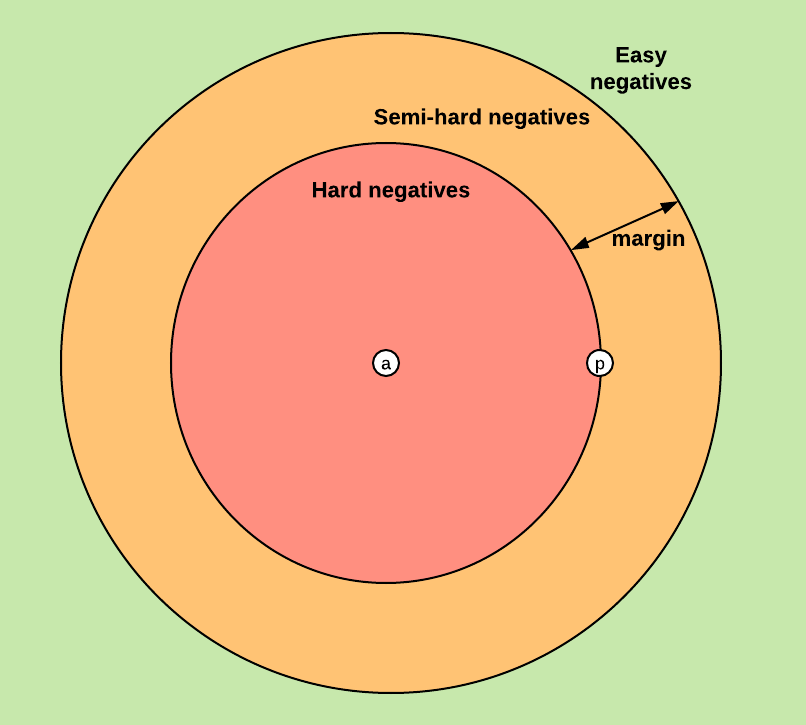
\includegraphics[width=120mm, keepaspectratio]{figures/triplet_type.png}
	\caption{A tripletek három típusa.}
	\label{fig:triplet-type}
\end{figure}

\ \\
Nehéz tripletek bányászása egy külön feladat és léteznek módszerek ún. offline (tanítás előtti) és online (tanítás közbeni) generálásra. Előnye, hogy gyorsabban konvergál a hálózat a veszteség minimuma felé. Ugyanakkor a FaceNet megjegyzi, hogy nehéz tripletekkel való tanítás az elején rossz lokális minimumhoz vezethet, ezért a félnehéz tripleteket ajánlja.

\subsubsection{Voicemap implementáció}

Létrehoztam egy bemenetként tripleteket fogadó neurális hálózatot \emph{triplet loss} veszteségfüggvénnyel (a triplet loss veszteségfüggvény részletes leírása a \ref{section:siamese_conv} fejezetben található). Egy bemenet egy olyan hangminta hármas (triplet), ami két azonos és egy különbözőtől beszélőtől tartalmaz hangmintát. 
\newline
\newline
A két azonos minta közül az egyik lesz az \emph{anchor} érték. Ehhez mérten számoljuk ki a pozitív (azonos beszélőtől származó) és negatív (különböző beszélőtől származó) távolságokat. 
\newline
\newline
Az alapja a konvolúciós enkóder. Ehhez csatlakozik három bemenet, a kimenetére pedig két lambda réteg ami a pozitív és negatív távolságokat számolja ki, majd még két lambda réteg kiszámolja a vektorok hosszát. A szubtrakciós réteg ezután a két kiszámolt vektort kivonja egymásból, ahogy a \ref{fig:triplet-network} ábrán látható.

\begin{figure}[!ht]
	\centering
	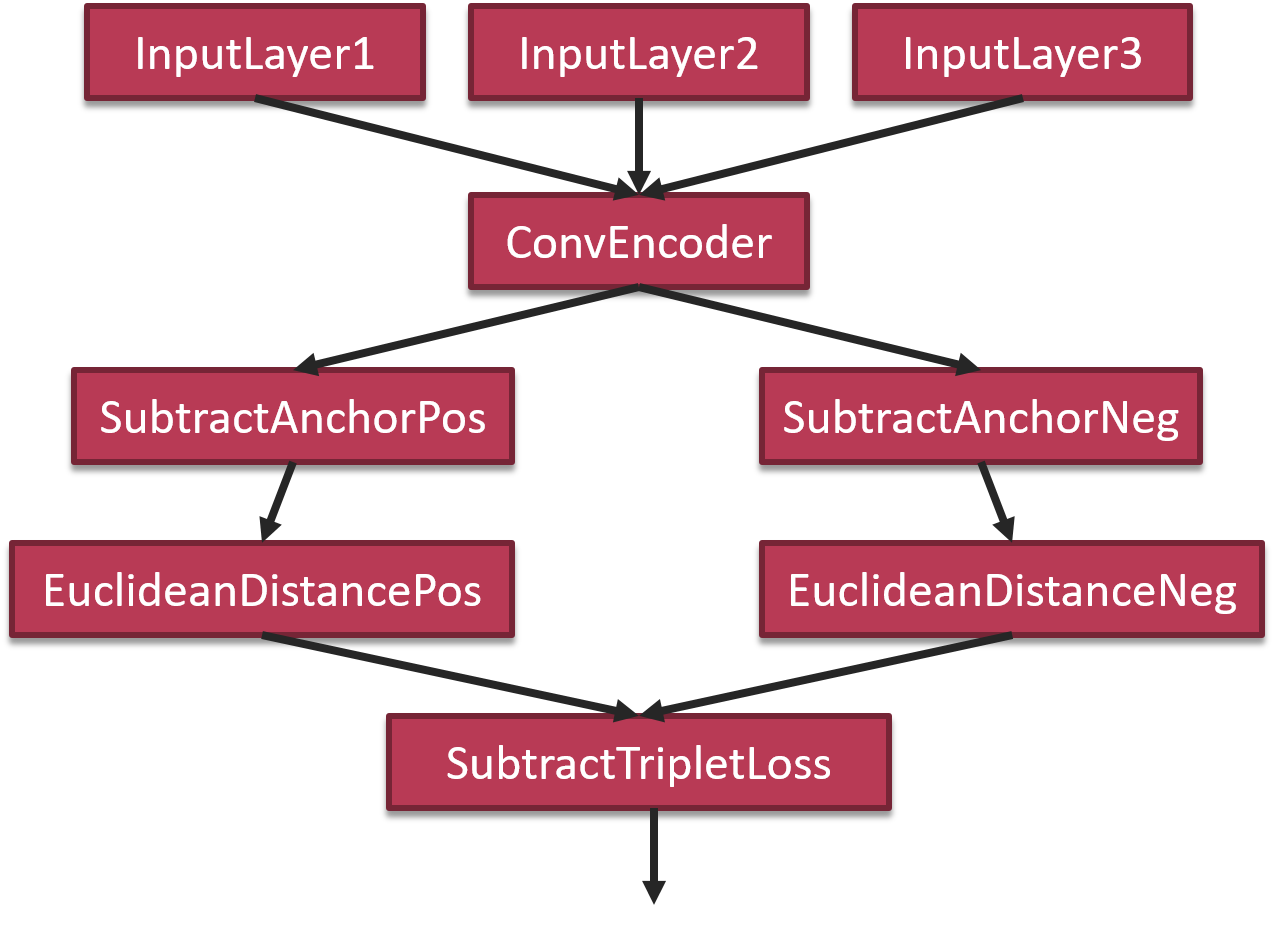
\includegraphics[width=120mm, keepaspectratio]{figures/triplet-network.png}
	\caption{Triplet hálózat.}
	\label{fig:triplet-network}
\end{figure}
\ \\
Tanításhoz a LibriSpeech adatbázist használtam. Ehhez módosítottam a \emph{LibriSpeechDataset} osztályt úgy, hogy képes legyen tripletekből álló batchek generálására is.
\newline
\newline
Az \emph{utils.py}-ben implementáltam magát a \emph{triplet loss} veszteségfüggvényt, módosítottam a BatchPreProcessor wrapper osztályt, hogy egységesen kezelje a triplet alakú tanítóadatokat a sziámi és sima konvolúciós bemenetekkel együtt, majd kiegészítettem az \emph{n\_shot\_task\_evaluation} függvényt úgy, hogy képes legyen \emph{k-way n-shot} feladat kiértékelést tripleteken is elvégezni.

\begin{figure}[!ht]
	\centering
	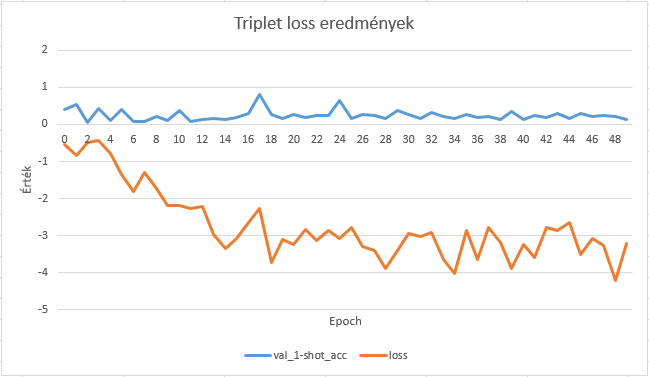
\includegraphics[width=150mm, keepaspectratio]{figures/triplet-loss-chart.png}
	\caption{Triplet lossal tanítás eredményei.}
	\label{fig:triplet-loss-chart}
\end{figure}
\ \\
A tanítás során minden batch végén 1-shot 5-way kiértékelés történik, azaz 5 beszélőtől egyelemű segédhalmazokkal próbálja a hálózat megtippelni, hogy melyik beszélőhöz tartozik a kérdéses hangminta.
\newline
\newline
A \ref{fig:triplet-loss-chart} grafikon azt mutatja, hogy az egyes epochok szerint hogyan változik a veszteség és a 1-shot 5-way pontosság. Látható, hogy a veszteség stagnálva, de csökken, ennek ellenére a validációs pontosság folyamatosan 0 és 1 között változik. A 17. és 24 epochnál megközelíti az 1-et, majd tovább romlik. A pontosság és a veszteség nem lassan, hanem egyáltalán nem konvergál, ezért feltételezhető, hogy nem a véletlenszerű tripletek kiválasztása a probléma. A tanítás nem volt sikeres.
%%----------------------------------------------------------------------------
\chapter{\bevezetes}
%----------------------------------------------------------------------------

A bevezető tartalmazza a diplomaterv-kiírás elemzését, történelmi előzményeit, a feladat indokoltságát (a motiváció leírását), az eddigi megoldásokat, és ennek tükrében a hallgató megoldásának összefoglalását.

A bevezető szokás szerint a diplomaterv felépítésével záródik, azaz annak rövid leírásával, hogy melyik fejezet mivel foglalkozik.

%%----------------------------------------------------------------------------
\chapter{\LaTeX-eszközök}
\label{sec:LatexTools}
%----------------------------------------------------------------------------
\section{A szerkesztéshez használatos eszközök}
%----------------------------------------------------------------------------
Ez a sablon TeXstudio 2.8.8 szerkesztővel készült. A TeXstudio egy platformfüggetlen, Windows, Linux és Mac OS alatt is elérhető \LaTeX-szerkesztőprogram számtalan hasznos szolgáltatással (\refstruc{fig:TeXstudio}). A szoftver ingyenesen letölthető\footnote{A TeXstudio hivatalos oldala: \url{http://texstudio.sourceforge.net/}}.

\begin{figure}[!ht]
\centering
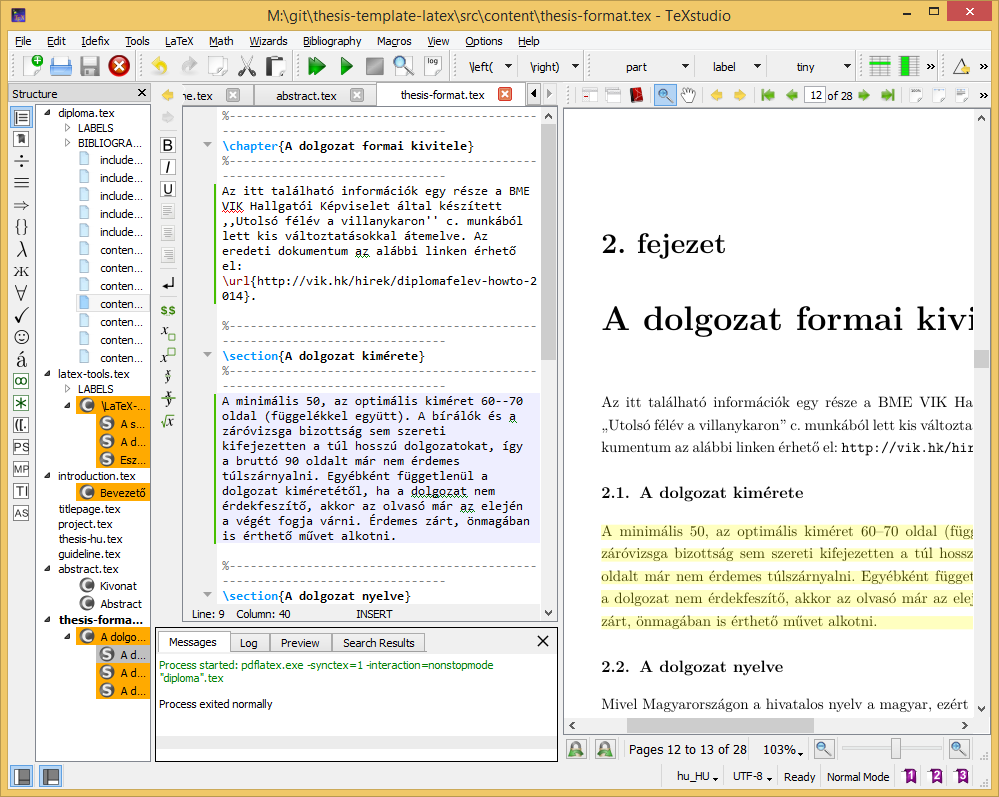
\includegraphics[width=150mm, keepaspectratio]{figures/TeXstudio.png}
\caption{A TeXstudio \LaTeX-szerkesztő.}
\label{fig:TeXstudio}
\end{figure}

A TeXstudio telepítése után érdemes még letölteni a magyar nyelvű helyesírásellenőrző-szótárakat hozzá. A TeXstudio az OpenOffice-hoz használatos formátumot tudja kezelni. A TeXstudio beállításainál a \verb+General+ fülön a \verb+Dictionaries+ résznél tudjuk megadni, hogy melyik szótárat használja.

Egy másik használható Windows alapú szerkesztőprogram a LEd\footnote{A LEd hivatalos oldala: \url{http://www.latexeditor.org/}} (LaTeX Editor), a TeXstudio azonban stabilabb, gyorsabb, és jobban használható.

%----------------------------------------------------------------------------
\section{A dokumentum lefordítása Windows alatt}
%----------------------------------------------------------------------------
A TeXstudio és a LEd kizárólag szerkesztőprogram (bár az utóbbiban DVI-nézegető is van), így a dokumentum fordításához szükséges eszközöket nem tartalmazza. Windows alatt alapvetően két lehetőség közül érdemes választani: MiKTeX (\url{http://miktex.org/}) és TeX Live (\url{http://www.tug.org/texlive/}) programcsomag. Az utóbbi működik Mac OS X, GNU/Linux alatt és Unix-származékokon is. A MiKTeX egy alapcsomag telepítése után mindig letölti a használt funkciókhoz szükséges, de lokálisan hiányzó \TeX-csomagokat, míg a TeX Live DVD ISO verzóban férhető hozzá. Ez a dokumentum TeX Live 2008 programcsomag segítségével fordult, amelynek DVD ISO verziója a megadott oldalról letölthető. A sablon lefordításához a disztribúcióban szereplő \verb+magyar.ldf+ fájlt a \verb+http://www.math.bme.hu/latex/+ változatra kell cserélni, vagy az utóbbi változatot be kell másolni a projekt-könyvtárba (ahogy ezt meg is tettük a sablonban) különben anomáliák tapasztalhatók a dokumentumban (pl. az ábra- és táblázat-aláírások formátuma nem a beállított lesz, vagy bizonyos oldalakon megjelenik alapértelmezésben egy fejléc). A TeX Live 2008-at még nem kell külön telepíteni a gépre, elegendő DVD-ről (vagy az ISO fájlból közvetlenül, pl. DaemonTools-szal) használni.

Ha a MiKTeX csomagot használjuk, akkor parancssorból a következő módon tudjuk újrafordítani a teljes dokumentumot:

\begin{lstlisting}[language=bash,frame=single,float=!ht]
$ texify -p thesis.tex
\end{lstlisting}

A \verb+texify+ parancs a MiKTex programcsomag \verb+miktex/bin+ alkönyvtárában található. A parancs gondoskodik arról, hogy a szükséges lépéseket (fordítás, hivatkozások generálása stb.) a megfelelő sorrendben elvégezze. A \verb+-p+ kapcsoló hatására PDF-et generál. A fordítást és az ideiglenes fájlok törlését elvégezhetjük a sablonhoz mellékelt \verb+manual_build.bat+ szkript segítségével is.

A \TeX-eszközöket tartalmazó programcsomag binárisainak elérési útját gyakran be kell állítani a szerkesztőprogramban, például TeXstudio esetén legegyszerűbben az \verb+Options / Configure TeXstudio... / Commands+ menüponttal előhívott dialógusablakban tehetjük ezt meg.

A PDF-\LaTeX~használata esetén a generált dokumentum közvetlenül PDF-formátumban áll rendelkezésre. Amennyiben a PDF-fájl egy PDF-nézőben (pl. Adobe Acrobat Reader vagy Foxit PDF Reader) meg van nyitva, akkor a fájlleírót a PDF-néző program tipikusan lefoglalja. Ilyen esetben a dokumentum újrafordítása hibaüzenettel kilép. Ha bezárjuk és újra megnyitjuk a PDF dokumentumot, akkor pedig a PDF-nézők többsége az első oldalon nyitja meg a dokumentumot, nem a legutóbb olvasott oldalon. Ezzel szemben például az egyszerű és ingyenes \textcolor{blue}{Sumatra PDF} nevű program képes arra, hogy a megnyitott dokumentum megváltozását detektálja, és frissítse a nézetet az aktuális oldal megtartásával.

%----------------------------------------------------------------------------
\section{Eszközök Linuxhoz}
%----------------------------------------------------------------------------
Linux operációs rendszer alatt is rengeteg szerkesztőprogram van, pl. a KDE alapú Kile jól használható. Ez ingyenesen letölthető, vagy éppenséggel az adott Linux-disztribúció eleve tartalmazza, ahogyan a dokumentum fordításához szükséges csomagokat is. Az Ubuntu Linux disztribúciók alatt például legtöbbször a \verb+texlive-*+ csomagok telepítésével használhatók a \LaTeX-eszközök. A jelen sablon fordításához szükséges csomagok (kb. 0,5 GB) az alábbi paranccsal telepíthetők:

\begin{lstlisting}[language=bash,morekeywords={sudo,apt\-get},alsoletter={-},breaklines=true]
$ sudo apt-get install texlive-latex-extra texlive-fonts-extra texlive-fonts-recommended texlive-xetex texlive-science
\end{lstlisting}

Amennyiben egy újabb csomag hozzáadása után hiányzó fájlra utaló hibát kapunk a fordítótól, telepítenünk kell az azt tartalmazó TeX Live csomagot. Ha pl. a \verb+bibentry+ csomagot szeretnénk használni, futtassuk az alábbi parancsot:

\begin{lstlisting}[language=bash,morekeywords={apt\-cache},alsoletter={-},breaklines=true]
$ apt-cache search bibentry
texlive-luatex - TeX Live: LuaTeX packages
\end{lstlisting}

Majd telepítsük fel a megfelelő TeX Live csomagot, jelen esetben a `texlive-lualatex`-et. (Egy LaTeX csomag több TeX Live csomagban is szerepelhet.)

Ha gyakran szerkesztünk más \LaTeX dokumentumokat is, kényelmes és biztos megoldás a teljes TeX Live disztribúció telepítése, ez azonban kb. 4 GB helyet igényel.

\begin{lstlisting}[language=bash,morekeywords={sudo,apt\-get},alsoletter={-},breaklines=true]
sudo apt-get install texlive-full
\end{lstlisting}

%%----------------------------------------------------------------------------
\chapter{A dolgozat formai kivitele}
%----------------------------------------------------------------------------
Az itt található információk egy része a BME VIK Hallgatói Képviselet által készített ,,Utolsó félév a villanykaron'' c. munkából lett kis változtatásokkal átemelve. Az eredeti dokumentum az alábbi linken érhető el: \url{http://vik.hk/hirek/diplomafelev-howto-2015}.

%----------------------------------------------------------------------------
\section{A dolgozat kimérete}
%----------------------------------------------------------------------------
Szakdolgozat esetében minimum 30, 45 körüli ajánlott oldalszám lehet az iránymutató. De mindenképp érdemes rákérdezni a konzulensnél is az elvárásokra, mert tanszékenként változóak lehetnek az elvárások.

Mesterképzésen a Diplomatervezés 1 esetében a beszámoló még inkább az Önálló laboratóriumi beszámolókhoz hasonlít, tanszékenként eltérő formai követelményekkel, -- egy legalább 30 oldal körüli dolgozat az elvárt -- és az elmúlt fél éves munkáról szól. De egyben célszerű, ha ez a végleges diplomaterv alapja is. (A végleges 60-90 oldal körülbelül a hasznos részre nézve)


%----------------------------------------------------------------------------
\section{A dolgozat nyelve}
%----------------------------------------------------------------------------
Mivel Magyarországon a hivatalos nyelv a magyar, ezért alapértelmezésben magyarul kell megírni a dolgozatot. Aki külföldi posztgraduális képzésben akar részt venni, nemzetközi szintű tudományos kutatást szeretne végezni, vagy multinacionális cégnél akar elhelyezkedni, annak célszerű angolul megírnia diplomadolgozatát. Mielőtt a hallgató az angol nyelvű verzió mellett dönt, erősen ajánlott mérlegelni, hogy ez mennyi többletmunkát fog a hallgatónak jelenteni fogalmazás és nyelvhelyesség terén, valamint -- nem utolsó sorban -- hogy ez mennyi többletmunkát fog jelenteni a konzulens illetve bíráló számára. Egy nehezen olvasható, netalán érthetetlen szöveg teher minden játékos számára.

%----------------------------------------------------------------------------
\section{A dokumentum nyomdatechnikai kivitele}
%----------------------------------------------------------------------------
A dolgozatot A4-es fehér lapra nyomtatva, 2,5 centiméteres margóval (+1~cm kötésbeni), 11--12 pontos betűmérettel, talpas betűtípussal és másfeles sorközzel célszerű elkészíteni.

Annak érdekében, hogy a dolgozat külsőleg is igényes munka benyomását keltse, érdemes figyelni az alapvető tipográfiai szabályok betartására~\cite{Jeney}.

%% !TeX spellcheck = hu_HU
% !TeX encoding = UTF-8
% !TeX program = xelatex
%----------------------------------------------------------------------------
\chapter{A \LaTeX-sablon használata}
%----------------------------------------------------------------------------

Ebben a fejezetben röviden, implicit módon bemutatjuk a sablon használatának módját, ami azt jelenti, hogy sablon használata ennek a dokumentumnak a forráskódját tanulmányozva válik teljesen világossá. Amennyiben a szoftver-keretrendszer telepítve van, a sablon alkalmazása és a dolgozat szerkesztése \LaTeX-ben a sablon segítségével tapasztalataink szerint jóval hatékonyabb, mint egy WYSWYG (\emph{What You See is What You Get}) típusú szövegszerkesztő esetén (pl. Microsoft Word, OpenOffice).

%----------------------------------------------------------------------------
\section{Címkék és hivatkozások}
%----------------------------------------------------------------------------
A \LaTeX~dokumentumban címkéket (\verb+\label+) rendelhetünk ábrákhoz, táblázatokhoz, fejezetekhez, listákhoz, képletekhez stb. Ezekre a dokumentum bármely részében hivatkozhatunk, a hivatkozások automatikusan feloldásra kerülnek.

A sablonban makrókat definiáltunk a hivatkozások megkönnyítéséhez. Ennek megfelelően minden ábra (\emph{figure}) címkéje \verb+fig:+ kulcsszóval kezdődik, míg minden táblázat (\emph{table}), képlet (\emph{equation}), fejezet (\emph{section}) és lista (\emph{listing}) rendre a \verb+tab:+, \verb+eq:+, \verb+sec:+ és \verb+lst:+ kulcsszóval kezdődik, és a kulcsszavak után tetszőlegesen választott címke használható. Ha ezt a konvenciót betartjuk, akkor az előbbi objektumok számára rendre a \verb+\figref+, \verb+\tabref+, \verb+\eqref+, \verb+\sectref+ és \verb+\listref+ makrókkal hivatkozhatunk. A makrók paramétere a címke, amelyre hivatkozunk (a kulcsszó nélkül). Az összes említett hivatkozástípus, beleértve az \verb+\url+ kulcsszóval bevezetett web-hivatkozásokat is a  \verb+hyperref+\footnote{Segítségével a dokumentumban megjelenő hivatkozások nem csak dinamikussá válnak, de színezhetők is, bővebbet erről a csomag dokumentációjában találunk. Ez egyúttal egy példa lábjegyzet írására.} csomagnak köszönhetően aktívak a legtöbb PDF-nézegetőben, rájuk kattintva a dokumentum megfelelő oldalára ugrik a PDF-néző vagy a megfelelő linket megnyitja az alapértelmezett böngészővel. A \verb+hyperref+ csomag a kimeneti PDF-dokumentumba könyvjelzőket is készít a tartalomjegyzékből. Ez egy szintén aktív tartalomjegyzék, amelynek elemeire kattintva a nézegető behozza a kiválasztott fejezetet.

%----------------------------------------------------------------------------
\section{Ábrák és táblázatok}
%----------------------------------------------------------------------------
Használjunk vektorgrafikus ábrákat, ha van rá módunk. PDFLaTeX használata esetén PDF formátumú ábrákat lehet beilleszteni könnyen, az EPS (PostScript) vektorgrafikus képformátum beillesztését a PDFLaTeX közvetlenül nem támogatja (de lehet konvertálni, lásd később). Ha vektorgrafikus formában nem áll rendelkezésünkre az ábra, akkor a  veszteségmentes PNG, valamint a veszteséges JPEG formátumban érdemes elmenteni.  Figyeljünk arra, hogy ilyenkor a képek felbontása elég nagy legyen ahhoz, hogy nyomtatásban is megfelelő minőséget nyújtson (legalább 300 dpi javasolt). A dokumentumban felhasznált képfájlokat a dokumentum forrása mellett érdemes tartani, archiválni, mivel ezek hiányában a dokumentum nem fordul újra. Ha lehet, a vektorgrafikus képeket vektorgrafikus formátumban is érdemes elmenteni az újrafelhasználhatóság (az átszerkeszthetőség) érdekében.

Kapcsolási rajzok legtöbbször kimásolhatók egy vektorgrafikus programba (pl. CorelDraw) és onnan nagyobb felbontással raszterizálva kimenthatők PNG formátumban. Ugyanakkor kiváló ábrák készíthetők Microsoft Visio vagy hasonló program használatával is: Visio-ból az ábrák közvetlenül PDF-be is menthetők.

Lehetőségeink Matlab ábrák esetén:
\begin{itemize}
	\item Képernyőlopás (\emph{screenshot}) is elfogadható minőségű lehet a dokumentumban, de általában jobb felbontást is el lehet érni más módszerrel.
	\item A Matlab ábrát a \verb+File/Save As+ opcióval lementhetjük PNG formátumban (ugyanaz itt is érvényes, mint korábban, ezért nem javasoljuk).
	\item A Matlab ábrát az \verb+Edit/Copy figure+ opcióval kimásolhatjuk egy vektorgrafikus programba is és onnan nagyobb felbontással raszterizálva kimenthatjük PNG formátumban (nem javasolt).
	\item Javasolt megoldás: az ábrát a \verb+File/Save As+ opcióval EPS \emph{vektorgrafikus} formátumban elmentjük, PDF-be konvertálva beillesztjük a dolgozatba.
\end{itemize}
Az EPS kép az \verb+epstopdf+ programmal\footnote{a korábban említett \LaTeX-disztribúciókban megtalálható} konvertálható PDF formátumba. Célszerű egy batch-fájlt készíteni az összes EPS ábra lefordítására az alábbi módon (ez Windows alatt működik).
\begin{lstlisting}[language=]
@echo off
for %%j in (*.eps) do (
  echo converting file "%%j"
  epstopdf "%%j"
)
echo done .
\end{lstlisting}

Egy ilyen parancsfájlt (\verb+convert.cmd+) elhelyeztük a sablon \verb+figures\eps+ könyvtárába, így a felhasználónak csak annyi a dolga, hogy a \verb+figures\eps+ könyvtárba kimenti az EPS formátumú vektorgrafikus képet, majd lefuttatja a \verb+convert.cmd+ parancsfájlt, ami PDF-be konvertálja az EPS fájlt.

Ezek után a PDF-ábrát ugyanúgy lehet a dokumentumba beilleszteni, mint a PNG-t vagy a JPEG-et. A megoldás előnye, hogy a lefordított dokumentumban is vektorgrafikusan tárolódik az ábra, így a mérete jóval kisebb, mintha raszterizáltuk volna beillesztés előtt. Ez a módszer minden -- az EPS formátumot ismerő -- vektorgrafikus program (pl. CorelDraw) esetén is használható.

A képek beillesztésére \az+\refstruc{sec:LatexTools}ben mutattunk be példát (\refstruc{fig:TeXstudio}). Az előző mondatban egyúttal az automatikusan feloldódó ábrahivatkozásra is láthatunk példát. Több képfájlt is beilleszthetünk egyetlen ábrába. Az egyes képek közötti horizontális és vertikális margót metrikusan szabályozhatjuk (\refstruc{fig:HVSpaces}). Az ábrák elhelyezését számtalan tipográfiai szabály egyidejű teljesítésével a fordító maga végzi, a dokumentum írója csak preferenciáit jelezheti a fordító felé (olykor ez bosszúságot is okozhat, ilyenkor pl. a kép méretével lehet játszani).

\begin{figure}[!ht]
	\centering
	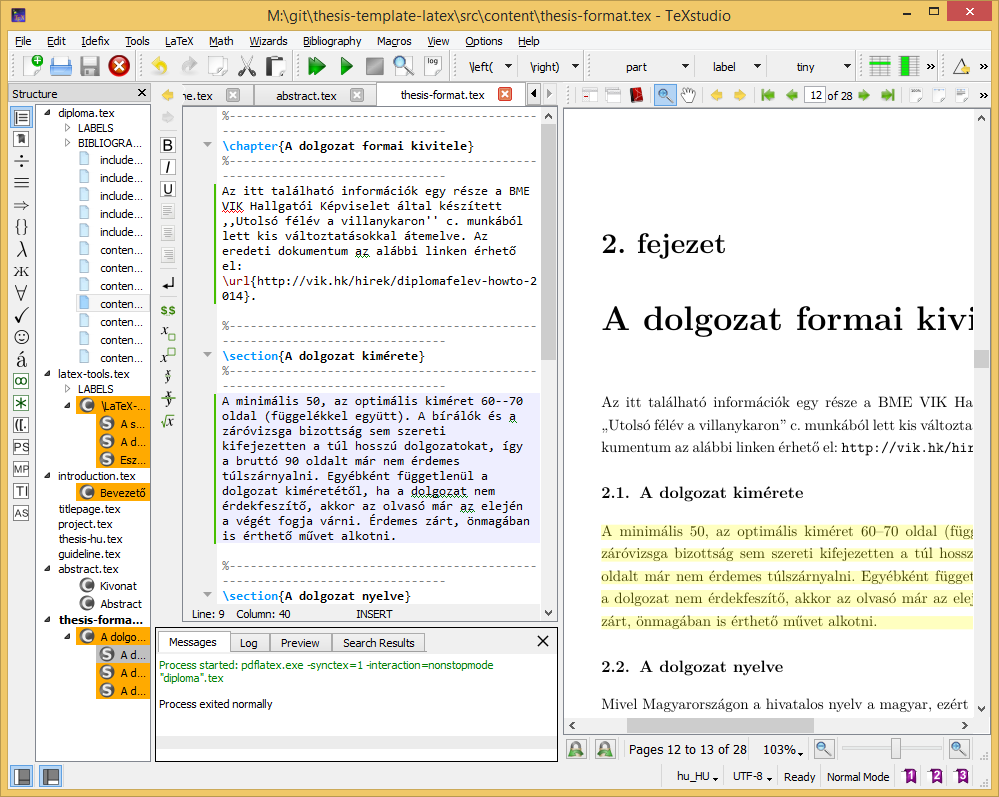
\includegraphics[width=67mm, keepaspectratio]{figures/TeXstudio.png}\hspace{1cm}
	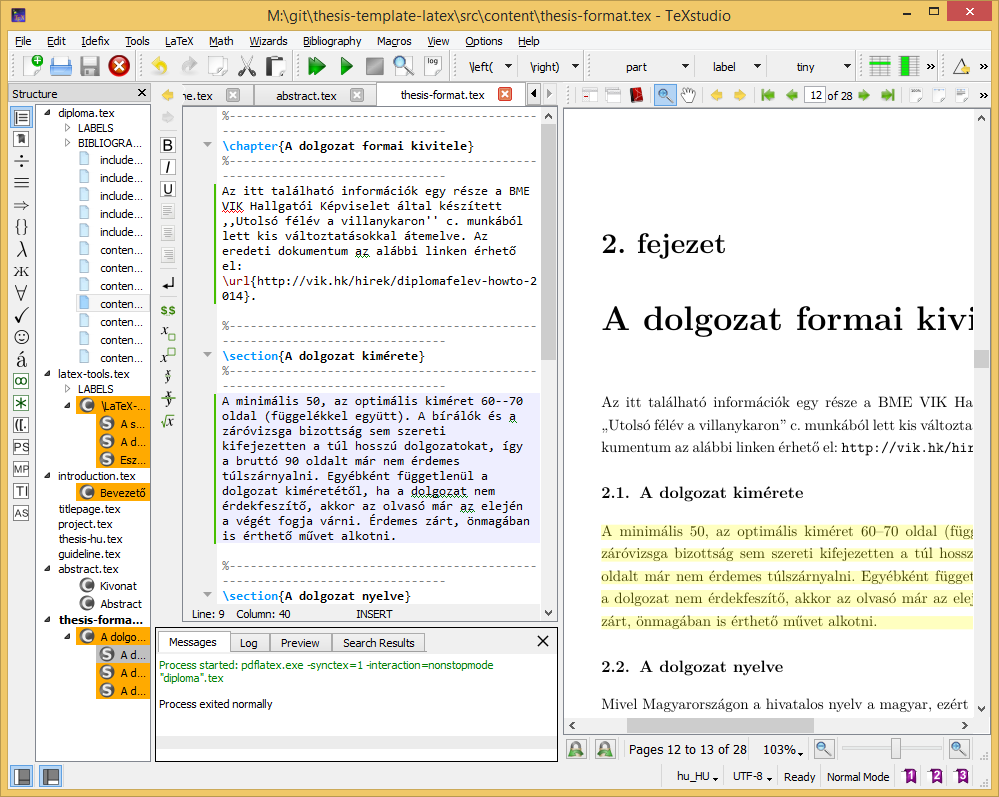
\includegraphics[width=67mm, keepaspectratio]{figures/TeXstudio.png}\\\vspace{5mm}
	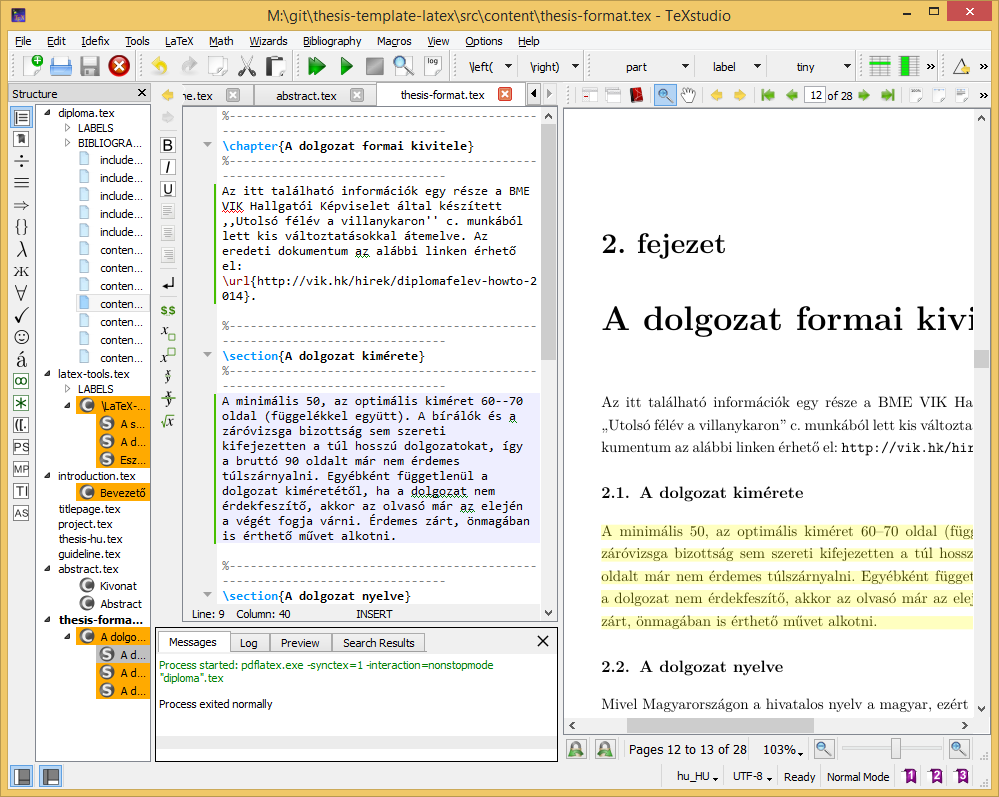
\includegraphics[width=67mm, keepaspectratio]{figures/TeXstudio.png}\hspace{1cm}
	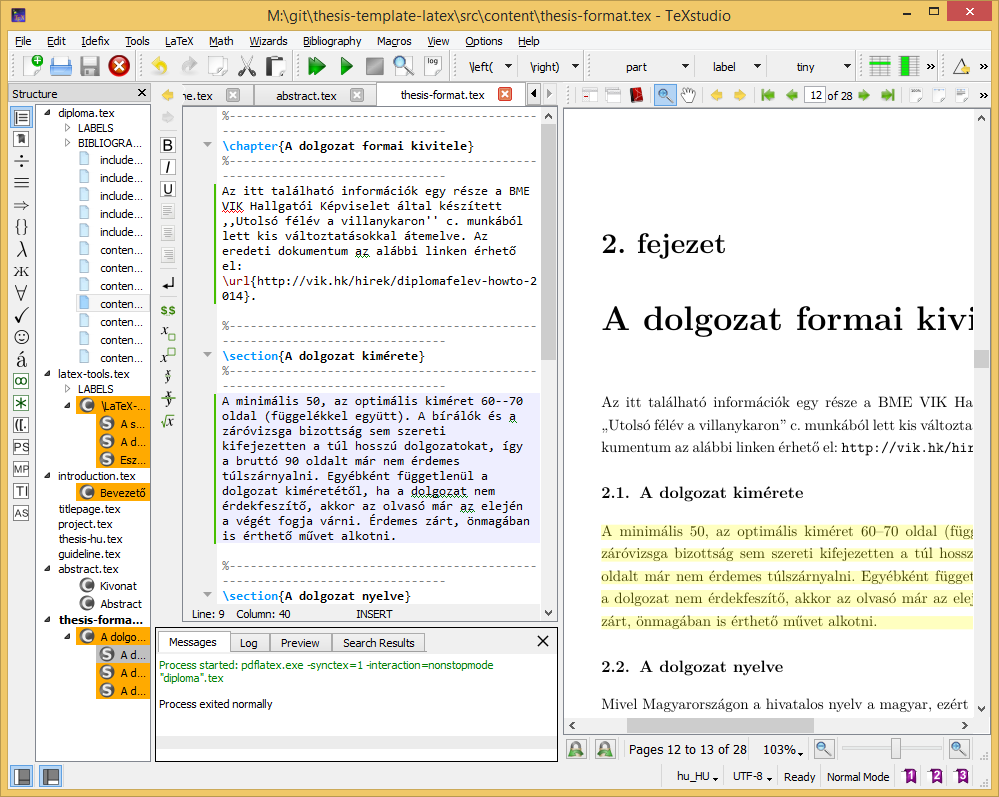
\includegraphics[width=67mm, keepaspectratio]{figures/TeXstudio.png}
	\caption{Több képfájl beillesztése esetén térközöket is érdemes használni.}
	\label{fig:HVSpaces}
\end{figure}

A táblázatok használatára \aref{tab:TabularExample}~táblázat mutat példát. A táblázatok formázásához hasznos tanácsokat találunk a \verb+booktabs+ csomag dokumentációjában.

\begin{table}[ht]
	\footnotesize
	\centering
	\begin{tabular}{ l c c }
		\toprule
		Órajel & Frekvencia & Cél pin \\
		\midrule
		CLKA & 100 MHz & FPGA CLK0\\
		CLKB & 48 MHz  & FPGA CLK1\\
		CLKC & 20 MHz  & Processzor\\
		CLKD & 25 MHz  & Ethernet chip \\
		CLKE & 72 MHz  & FPGA CLK2\\
		XBUF & 20 MHz  & FPGA CLK3\\
		\bottomrule
	\end{tabular}
	\caption{Az órajel-generátor chip órajel-kimenetei.}
	\label{tab:TabularExample}
\end{table}


%----------------------------------------------------------------------------
\section{Felsorolások és listák}
%----------------------------------------------------------------------------
Számozatlan felsorolásra mutat példát a jelenlegi bekezdés:
\begin{itemize}
	\item \emph{első bajusz:} ide lehetne írni az első elem kifejését,
	\item \emph{második bajusz:} ide lehetne írni a második elem kifejését,
	\item \emph{ez meg egy szakáll:} ide lehetne írni a harmadik elem kifejését.
\end{itemize}

Számozott felsorolást is készíthetünk az alábbi módon:
\begin{enumerate}
	\item \emph{első bajusz:} ide lehetne írni az első elem kifejését, és ez a kifejtés így néz ki, ha több sorosra sikeredik,
	\item \emph{második bajusz:} ide lehetne írni a második elem kifejését,
	\item \emph{ez meg egy szakáll:} ide lehetne írni a harmadik elem kifejését.
\end{enumerate}
A felsorolásokban sorok végén vessző, az utolsó sor végén pedig pont a szokásos írásjel. Ez alól kivételt képezhet, ha az egyes elemek több teljes mondatot tartalmaznak.

Listákban a dolgozat szövegétől elkülönítendő kódrészleteket, programsorokat, pszeudo-kódokat jeleníthetünk meg (\ref{lst:Example}.~kódrészlet).
\begin{lstlisting}[language=tex,caption=A fenti számozott felsorolás \LaTeX-forráskódja,label=lst:Example]
\begin{enumerate}
	\item \emph{els(*@ő@*) bajusz:} ide lehetne írni az els(*@ő@*) elem kifejését,
	és ez a kifejtés így néz ki, ha több sorosra sikeredik,
	\item \emph{második bajusz:} ide lehetne írni a második elem kifejését,
	\item \emph{ez meg egy szakáll:} ide lehetne írni a harmadik elem kifejését.
\end{enumerate}
\end{lstlisting}
A lista keretét, háttérszínét, egész stílusát megválaszthatjuk. Ráadásul különféle programnyelveket és a nyelveken belül kulcsszavakat is definiálhatunk, ha szükséges. Erről bővebbet a \verb+listings+ csomag hivatalos leírásában találhatunk.

%----------------------------------------------------------------------------
\section{Képletek}
%----------------------------------------------------------------------------
Ha egy formula nem túlságosan hosszú, és nem akarjuk hivatkozni a szövegből, mint például a $e^{i\pi}+1=0$ képlet, \emph{szövegközi képletként} szokás leírni. Csak, hogy másik példát is lássunk, az $U_i=-d\Phi/dt$ Faraday-törvény a $\rot E=-\frac{dB}{dt}$ differenciális alakban adott Maxwell-egyenlet felületre vett integráljából vezethető le. Látható, hogy a \LaTeX-fordító a sorközöket betartja, így a szöveg szedése esztétikus marad szövegközi képletek használata esetén is.

Képletek esetén az általános konvenció, hogy a kisbetűk skalárt, a kis félkövér betűk ($\mathbf{v}$) oszlopvektort -- és ennek megfelelően $\mathbf{v}^T$ sorvektort -- a kapitális félkövér betűk ($\mathbf{V}$) mátrixot jelölnek. Ha ettől el szeretnénk térni, akkor az alkalmazni kívánt jelölésmódot célszerű külön alfejezetben definiálni. Ennek megfelelően, amennyiben $\mathbf{y}$ jelöli a mérések vektorát, $\mathbf{\vartheta}$ a paraméterek vektorát és $\hat{\mathbf{y}}=\mathbf{X}\vartheta$ a paraméterekben lineáris modellt, akkor a \emph{Least-Squares} értelemben optimális paraméterbecslő $\hat{\mathbf{\vartheta}}_{LS}=(\mathbf{X}^T\mathbf{X})^{-1}\mathbf{X}^T\mathbf{y}$ lesz.

Emellett kiemelt, sorszámozott képleteket is megadhatunk, ennél az \verb+equation+ és a \verb+eqnarray+ környezetek helyett a korszerűbb \verb+align+ környezet alkalmazását javasoljuk (több okból, különféle problémák elkerülése végett, amelyekre most nem térünk ki). Tehát
\begin{align}
\dot{\mathbf{x}}&=\mathbf{A}\mathbf{x}+\mathbf{B}\mathbf{u},\\
\mathbf{y}&=\mathbf{C}\mathbf{x},
\end{align}
ahol $\mathbf{x}$ az állapotvektor, $\mathbf{y}$ a mérések vektora és $\mathbf{A}$, $\mathbf{B}$ és $\mathbf{C}$ a rendszert leíró paramétermátrixok. Figyeljük meg, hogy a két egyenletben az egyenlőségjelek egymáshoz igazítva jelennek meg, mivel a mindkettőt az \& karakter előzi meg a kódban. Lehetőség van számozatlan kiemelt képlet használatára is, például
\begin{align}
\dot{\mathbf{x}}&=\mathbf{A}\mathbf{x}+\mathbf{B}\mathbf{u},\nonumber\\
\mathbf{y}&=\mathbf{C}\mathbf{x}\nonumber.
\end{align}
Mátrixok felírására az $\mathbf{A}\mathbf{x}=\mathbf{b}$ inhomogén lineáris egyenlet részletes kifejtésével mutatunk példát:
\begin{align}
\begin{bmatrix}
a_{11} & a_{12} & \dots & a_{1n}\\
a_{21} & a_{22} & \dots & a_{2n}\\
\vdots & \vdots & \ddots & \vdots\\
a_{m1} & a_{m2} & \dots & a_{mn}
\end{bmatrix}
\begin{pmatrix}x_1\\x_2\\\vdots\\x_n\end{pmatrix}=
\begin{pmatrix}b_1\\b_2\\\vdots\\b_m\end{pmatrix}.
\end{align}
A \verb+\frac+ utasítás hatékonyságát egy általános másodfokú tag átviteli függvényén keresztül mutatjuk be, azaz
\begin{align}
W(s)=\frac{A}{1+2T\xi s+s^2T^2}.
\end{align}
A matematikai mód minden szimbólumának és képességének a bemutatására természetesen itt nincs lehetőség, de gyors referenciaként hatékonyan használhatók a következő linkek:\\
\indent\url{http://www.artofproblemsolving.com/LaTeX/AoPS_L_GuideSym.php},\\
\indent\url{http://www.ctan.org/tex-archive/info/symbols/comprehensive/symbols-a4.pdf},\\
\indent\url{ftp://ftp.ams.org/pub/tex/doc/amsmath/short-math-guide.pdf}.\\
Ez pedig itt egy magyarázat, hogy miért érdemes \verb+align+ környezetet használni:\\
\indent\url{http://texblog.net/latex-archive/maths/eqnarray-align-environment/}.

%----------------------------------------------------------------------------
\section{Irodalmi hivatkozások}
\label{sec:HowtoReference}
%----------------------------------------------------------------------------
Egy \LaTeX~dokumentumban az irodalmi hivatkozások definíciójának két módja van. Az egyik a \verb+\thebibliograhy+ környezet használata a dokumentum végén, az \verb+\end{document}+ lezárás előtt.
\begin{lstlisting}[language=tex]
\begin{thebibliography}{9}

\bibitem{Lamport94} Leslie Lamport, \emph{\LaTeX: A Document Preparation System}.
Addison Wesley, Massachusetts, 2nd Edition, 1994.

\end{thebibliography}
\end{lstlisting}

Ezek után a dokumentumban a \verb+\cite{Lamport94}+ utasítással hivatkozhatunk a forrásra. A fenti megadás viszonylag kötetlen, a szerző maga formázza az irodalomjegyzéket (ami gyakran inkonzisztens eredményhez vezet).

Egy sokkal professzionálisabb módszer a BiB\TeX{} használata, ezért ez a sablon is ezt támogatja. Ebben az esetben egy külön szöveges adatbázisban definiáljuk a forrásmunkákat, és egy külön stílusfájl határozza meg az irodalomjegyzék kinézetét. Ez, összhangban azzal, hogy külön formátumkonvenció határozza meg a folyóirat-, a könyv-, a konferenciacikk- stb. hivatkozások kinézetét az irodalomjegyzékben (a sablon használata esetén ezzel nem is kell foglalkoznia a hallgatónak, de az eredményt célszerű ellenőrizni). felhasznált hivatkozások adatbázisa egy \verb+.bib+ kiterjesztésű szöveges fájl, amelynek szerkezetét a \Aref{lst:Bibtex} kódrészlet demonstrálja. A forrásmunkák bevitelekor a sor végi vesszők külön figyelmet igényelnek, mert hiányuk a BiB\TeX-fordító hibaüzenetét eredményezi. A forrásmunkákat típus szerinti kulcsszó vezeti be (\verb+@book+ könyv, \verb+@inproceedings+ konferenciakiadványban megjelent cikk, \verb+@article+ folyóiratban megjelent cikk, \verb+@techreport+ valamelyik egyetem gondozásában megjelent műszaki tanulmány, \verb+@manual+ műszaki dokumentáció esetén stb.). Nemcsak a megjelenés stílusa, de a kötelezően megadandó mezők is típusról-típusra változnak. Egy jól használható referencia a \url{http://en.wikipedia.org/wiki/BibTeX} oldalon található.

\begin{lstlisting}[caption=Példa szöveges irodalomjegyzék-adatbázisra Bib\TeX{} használata esetén.,label=lst:Bibtex]
@book{Wettl04,
  author    = {Ferenc Wettl and Gyula Mayer and Péter Szabó},
  publisher = {Panem Könyvkiadó},
  title     = {\LaTeX~kézikönyv},
  year      = {2004},
}

@article{Candy86,
  author       = {James C. Candy},
  journaltitle = {{IEEE} Trans.\ on Communications},
  month        = {01},
  note         = {\doi{10.1109/TCOM.1986.1096432}},
  number       = {1},
  pages        = {72--76},
  title        = {Decimation for Sigma Delta Modulation},
  volume       = {34},
  year         = {1986},
}

@inproceedings{Lee87,
  author    = {Wai L. Lee and Charles G. Sodini},
  booktitle = {Proc.\ of the IEEE International Symposium on Circuits and Systems},
  location  = {Philadelphia, PA, USA},
  month     = {05~4--7},
  pages     = {459--462},
  title     = {A Topology for Higher Order Interpolative Coders},
  vol       = {2},
  year      = {1987},
}

@thesis{KissPhD,
  author      = {Peter Kiss},
  institution = {Technical University of Timi\c{s}oara, Romania},
  month       = {04},
  title       = {Adaptive Digital Compensation of Analog Circuit Imperfections for Cascaded Delta-Sigma Analog-to-Digital Converters},
  type        = {phdthesis},
  year        = {2000},
}

@manual{Schreier00,
  author       = {Richard Schreier},
  month        = {01},
  note         = {\url{http://www.mathworks.com/matlabcentral/fileexchange/}},
  organization = {Oregon State University},
  title        = {The Delta-Sigma Toolbox v5.2},
  year         = {2000},
}

@misc{DipPortal,
  author       = {{Budapesti Műszaki és Gazdaságtudományi Egyetem Villamosmérnöki és Informatikai Kar}},
  howpublished = {\url{http://diplomaterv.vik.bme.hu/}},
  title        = {Diplomaterv portál (2011. február 26.)},
}

@incollection{Mkrtychev:1997,
  author    = {Mkrtychev, Alexey},
  booktitle = {Logical Foundations of Computer Science},
  doi       = {10.1007/3-540-63045-7_27},
  editor    = {Adian, Sergei and Nerode, Anil},
  isbn      = {978-3-540-63045-6},
  pages     = {266-275},
  publisher = {Springer Berlin Heidelberg},
  series    = {Lecture Notes in Computer Science},
  title     = {Models for the logic of proofs},
  url       = {http://dx.doi.org/10.1007/3-540-63045-7_27},
  volume    = {1234},
  year      = {1997},
}
\end{lstlisting}

A stílusfájl egy \verb+.sty+ kiterjesztésű fájl, de ezzel lényegében nem kell foglalkozni, mert vannak beépített stílusok, amelyek jól használhatók. Ez a sablon a BiB\TeX-et használja, a hozzá tartozó adatbázisfájl a \verb+mybib.bib+ fájl. Megfigyelhető, hogy az irodalomjegyzéket a dokumentum végére (a \verb+\end{document}+ utasítás elé) beillesztett \verb+\bibliography{mybib}+ utasítással hozhatjuk létre, a stílusát pedig ugyanitt a  \verb+\bibliographystyle{plain}+ utasítással adhatjuk meg. Ebben az esetben a \verb+plain+ előre definiált stílust használjuk (a sablonban is ezt állítottuk be). A \verb+plain+ stíluson kívül természetesen számtalan más előre definiált stílus is létezik. Mivel a \verb+.bib+ adatbázisban ezeket megadtuk, a BiB\TeX-fordító is meg tudja különböztetni a szerzőt a címtől és a kiadótól, és ez alapján automatikusan generálódik az irodalomjegyzék a stílusfájl által meghatározott stílusban.

Az egyes forrásmunkákra a szövegből továbbra is a \verb+\cite+ paranccsal tudunk hivatkozni, így \aref{lst:Bibtex}.~kódrészlet esetén a hivatkozások rendre \verb+\cite{Wettl04}+, \verb+\cite{Candy86}+, \verb+\cite{Lee87}+, \verb+\cite{KissPhD}+, \verb+\cite{Schreirer00}+,
\verb+\cite{Mkrtychev:1997}+ és \verb+\cite{DipPortal}+. Az egyes forrásmunkák sorszáma az irodalomjegyzék bővítésekor változhat. Amennyiben az aktuális számhoz illeszkedő névelőt szeretnénk használni, használjuk az \verb+\acite{}+ parancsot.

Az irodalomjegyzékben alapértelmezésben csak azok a forrásmunkák jelennek meg, amelyekre található hivatkozás a szövegben, és ez így alapvetően helyes is, hiszen olyan forrásmunkákat nem illik az irodalomjegyzékbe írni, amelyekre nincs hivatkozás.

Mivel a fordítási folyamat során több lépésben oldódnak fel a szimbólumok, ezért gyakran többször is le kell fordítani a dokumentumot. Ilyenkor ez első 1-2 fordítás esetleg szimbólum-feloldásra vonatkozó figyelmeztető üzenettel zárul. Ha hibaüzenettel zárul bármelyik fordítás, akkor nincs értelme megismételni, hanem a hibát kell megkeresni. A \verb+.bib+ fájl megváltoztatáskor sokszor nincs hatása a változtatásnak azonnal, mivel nem mindig fut újra a BibTeX fordító. Ezért célszerű a változtatás után azt manuálisan is lefuttatni (TeXstudio esetén \verb+Tools/Bibliography+).

Hogy a szövegbe ágyazott hivatkozások kinézetét demonstráljuk, itt most sorban meghivatkozzuk a \cite{Wettl04}, \cite{Candy86}, \cite{Lee87}, \cite{KissPhD}, \cite{Schreier00} és \acite{Mkrtychev:1997}\footnote{Informatikai témában gyakran hivatkozunk cikkeket a Springer LNCS valamely kötetéből, ez a hivatkozás erre mutat egy helyes példát.} forrásmunkát, valamint \acite{DipPortal} weboldalt.

Megjegyzendő, hogy az ékezetes magyar betűket is tartalmazó \verb+.bib+ fájl az \verb+inputenc+ csomaggal betöltött \verb+latin2+ betűkészlet miatt fordítható. Ugyanez a \verb+.bib+ fájl hibaüzenettel fordul egy olyan dokumentumban, ami nem tartalmazza a \verb+\usepackage[latin2]{inputenc}+ sort. Speciális igény esetén az irodalmi adatbázis általánosabb érvényűvé tehető, ha az ékezetes betűket speciális latex karakterekkel helyettesítjük a \verb+.bib+ fájlban, pl. á helyett \verb+\'{a}+-t vagy ő helyett \verb+\H{o}+-t írunk.

Irodalomhivatkozásokat célszerű először olyan szolgáltatásokban keresni, ahol jó minőségű bejegyzések találhatók (pl. ACM Digital Library,\footnote{\url{https://dl.acm.org/}} DBLP,\footnote{\url{http://dblp.uni-trier.de/}} IEEE Xplore,\footnote{\url{http://ieeexplore.ieee.org/}} SpringerLink\footnote{\url{https://link.springer.com/}}) és csak ezek után használni kevésbé válogatott forrásokat (pl. Google Scholar\footnote{\url{http://scholar.google.com/}}). A jó minőségű bejegyzéseket is érdemes megfelelően tisztítani.\footnote{\url{https://github.com/FTSRG/cheat-sheets/wiki/BibTeX-Fixing-entries-from-common-sources}} A sablon angol nyelvű változatában használt \texttt{plainnat} beállítás egyik sajátossága, hogy a cikkhez generált hivatkozás a cikk DOI-ját és URL-jét is tartalmazza, ami gyakran duplikátumhoz vezet -- érdemes tehát a DOI-kat tartalmazó URL mezőket törölni. 

%----------------------------------------------------------------------------
\section{A dolgozat szerkezete és a forrásfájlok}
%----------------------------------------------------------------------------
A diplomatervsablonban a TeX fájlok két alkönyvtárban helyezkednek el. Az \verb+include+ könyvtárban azok szerepelnek, amiket tipikusan nem kell szerkesztenünk, ezek a sablon részei (pl. címoldal). A \verb+content+ alkönyvtárban pedig a saját munkánkat helyezhetjük el. Itt érdemes az egyes fejezeteket külön \TeX{} állományokba rakni.

A diplomatervsablon (a kari irányelvek szerint) az alábbi fő fejezetekből áll:
\begin{enumerate}
	\item 1 oldalas \emph{tájékoztató} a szakdolgozat/diplomaterv szerkezetéről (\verb+include/guideline.tex+), ami a végső dolgozatból törlendő,
	\item \emph{feladatkiírás} (\verb+include/project.tex+), a dolgozat nyomtatott verzójában ennek a helyére kerül a tanszék által kiadott, a tanszékvezető által aláírt feladatkiírás, a dolgozat elektronikus verziójába pedig a feladatkiírás egyáltalán ne kerüljön bele, azt külön tölti fel a tanszék a diplomaterv-honlapra,
	\item \emph{címoldal} (\verb+include/titlepage.tex+),
	\item \emph{tartalomjegyzék} (\verb+thesis.tex+),
	\item a diplomatervező \emph{nyilatkozat}a az önálló munkáról (\verb+include/declaration.tex+),
	\item 1-2 oldalas tartalmi \emph{összefoglaló} magyarul és angolul, illetve elkészíthető még további nyelveken is (\verb+content/abstract.tex+),
	\item \emph{bevezetés}: a feladat értelmezése, a tervezés célja, a feladat indokoltsága, a diplomaterv felépítésének rövid összefoglalása (\verb+content/introduction.tex+),
	\item sorszámmal ellátott \emph{fejezetek}: a feladatkiírás pontosítása és részletes elemzése, előzmények (irodalomkutatás, hasonló alkotások), az ezekből levonható következtetések, a tervezés részletes leírása, a döntési lehetőségek értékelése és a választott megoldások indoklása, a megtervezett műszaki alkotás értékelése, kritikai elemzése, továbbfejlesztési lehetőségek,
	\item esetleges \emph{köszönetnyilvánítás}ok (\verb+content/acknowledgement.tex+),
	\item részletes és pontos \emph{irodalomjegyzék} (ez a sablon esetében automatikusan generálódik a \verb+thesis.tex+ fájlban elhelyezett \verb+\bibliography+ utasítás hatására, \az+\refstruc{sec:HowtoReference}ban leírtak szerint),
	\item \emph{függelékek} (\verb+content/appendices.tex+).
\end{enumerate}

A sablonban a fejezetek a \verb+thesis.tex+ fájlba vannak beillesztve \verb+\include+ utasítások segítségével. Lehetőség van arra, hogy csak az éppen szerkesztés alatt álló \verb+.tex+ fájlt fordítsuk le, ezzel lerövidítve a fordítási folyamatot. Ezt a lehetőséget az alábbi kódrészlet biztosítja a \verb+thesis.tex+ fájlban.
\begin{lstlisting}
\includeonly{
	guideline,%
	project,%
	titlepage,%
	declaration,%
	abstract,%
	introduction,%
	chapter1,%
	chapter2,%
	chapter3,%
	acknowledgement,%
	appendices,%
}
\end{lstlisting}

Ha az alábbi kódrészletben az egyes sorokat a \verb+%+ szimbólummal kikommentezzük, akkor a megfelelő \verb+.tex+ fájl nem fordul le. Az oldalszámok és a tartalomjegyék természetesen csak akkor billennek helyre, ha a teljes dokumentumot lefordítjuk.

%----------------------------------------------------------------------------
\newpage
\section{Alapadatok megadása}
%----------------------------------------------------------------------------
A diplomaterv alapadatait (cím, szerző, konzulens, konzulens titulusa) a \verb+thesis.tex+ fájlban lehet megadni.

%----------------------------------------------------------------------------
\section{Új fejezet írása}
%----------------------------------------------------------------------------
A főfejezetek külön \verb+content+ könyvtárban foglalnak helyet. A sablonhoz 3 fejezet készült. További főfejezeteket úgy hozhatunk létre, ha új \TeX~fájlt készítünk a fejezet számára, és a \verb+thesis.tex+ fájlban, a \verb+\include+ és \verb+\includeonly+ utasítások argumentumába felvesszük az új \verb+.tex+ fájl nevét.


%----------------------------------------------------------------------------
\section{Definíciók, tételek, példák}
%----------------------------------------------------------------------------

\begin{definition}[Fluxuskondenzátor térerőssége]
Lorem ipsum dolor sit amet, consectetur adipiscing elit, sed do eiusmod tempor incididunt ut labore et dolore magna aliqua. Ut enim ad minim veniam, quis nostrud exercitation ullamco laboris nisi ut aliquip ex ea commodo consequat.
\end{definition}

\begin{example}
Példa egy példára. Duis aute irure dolor in reprehenderit in voluptate velit esse cillum dolore eu fugiat nulla pariatur. Excepteur sint occaecat cupidatat non proident, sunt in culpa qui officia deserunt mollit anim id est laborum.
\end{example}

\begin{theorem}[Kovács tétele]
Duis aute irure dolor in reprehenderit in voluptate velit esse cillum dolore eu fugiat nulla pariatur. Excepteur sint occaecat cupidatat non proident, sunt in culpa qui officia deserunt mollit anim id est laborum.
\end{theorem}



% Acknowledgements
%~~~~~~~~~~~~~~~~~~~~~~~~~~~~~~~~~~~~~~~~~~~~~~~~~~~~~~~~~~~~~~~~~~~~~~~~~~~~~~~~~~~~~~
%----------------------------------------------------------------------------
\chapter*{\koszonetnyilvanitas}\addcontentsline{toc}{chapter}{\koszonetnyilvanitas}
%----------------------------------------------------------------------------

Ez nem kötelező, akár törölhető is. Ha a szerző szükségét érzi, itt lehet köszönetet nyilvánítani azoknak, akik hozzájárultak munkájukkal ahhoz, hogy a hallgató a szakdolgozatban vagy diplomamunkában leírt feladatokat sikeresen elvégezze. A konzulensnek való köszönetnyilvánítás sem kötelező, a konzulensnek hivatalosan is dolga, hogy a hallgatót konzultálja.


% List of Figures, Tables
%~~~~~~~~~~~~~~~~~~~~~~~~~~~~~~~~~~~~~~~~~~~~~~~~~~~~~~~~~~~~~~~~~~~~~~~~~~~~~~~~~~~~~~
%\listoffigures\addcontentsline{toc}{chapter}{\listfigurename}
%\listoftables\addcontentsline{toc}{chapter}{\listtablename}


% Bibliography
%~~~~~~~~~~~~~~~~~~~~~~~~~~~~~~~~~~~~~~~~~~~~~~~~~~~~~~~~~~~~~~~~~~~~~~~~~~~~~~~~~~~~~~
\addcontentsline{toc}{chapter}{\bibname}
\bibliography{bib/mybib}


% Appendix
%~~~~~~~~~~~~~~~~~~~~~~~~~~~~~~~~~~~~~~~~~~~~~~~~~~~~~~~~~~~~~~~~~~~~~~~~~~~~~~~~~~~~~~
%----------------------------------------------------------------------------
\appendix
%----------------------------------------------------------------------------
\chapter*{\fuggelek}\addcontentsline{toc}{chapter}{\fuggelek}
\setcounter{chapter}{\appendixnumber}
%\setcounter{equation}{0} % a fofejezet-szamlalo az angol ABC 6. betuje (F) lesz
\numberwithin{equation}{section}
\numberwithin{figure}{section}
\numberwithin{lstlisting}{section}
%\numberwithin{tabular}{section}

%----------------------------------------------------------------------------
\section{A TeXstudio felülete}
%----------------------------------------------------------------------------
\begin{figure}[!ht]
\centering
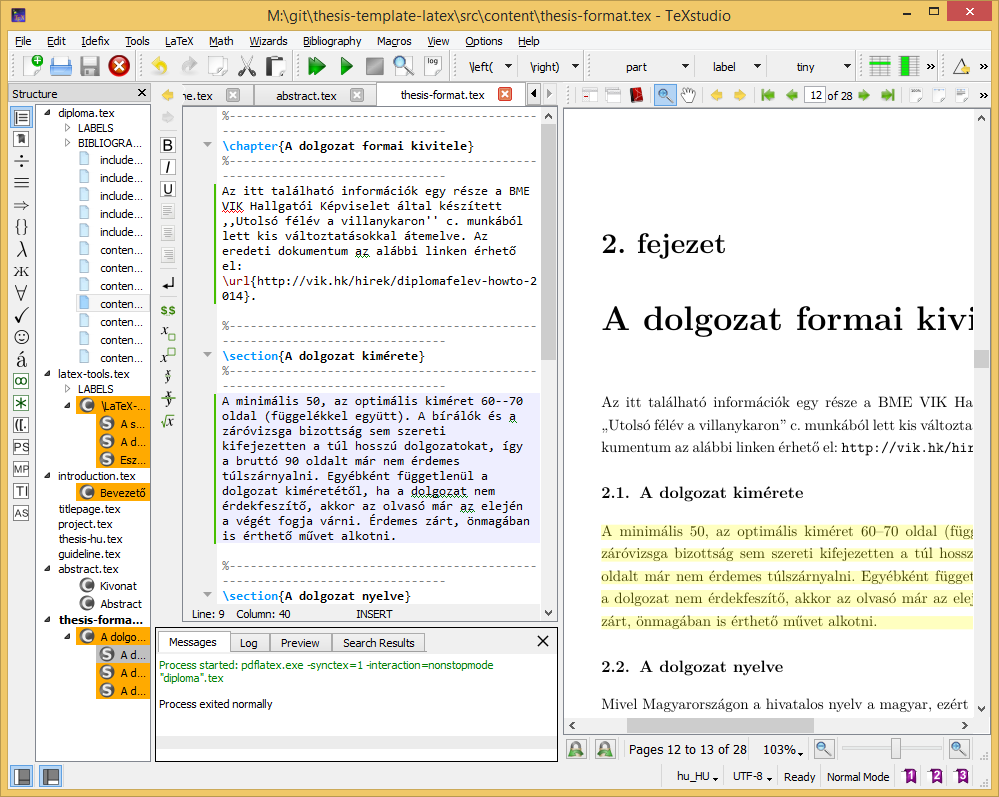
\includegraphics[width=150mm, keepaspectratio]{figures/TeXstudio.png}
\caption{A TeXstudio \LaTeX-szerkesztő.} 
\end{figure}

%----------------------------------------------------------------------------
\clearpage\section{Válasz az ,,Élet, a világmindenség, meg minden'' kérdésére}
%----------------------------------------------------------------------------
A Pitagorasz-tételből levezetve
\begin{align}
c^2=a^2+b^2=42.
\end{align}
A Faraday-indukciós törvényből levezetve
\begin{align}
\rot E=-\frac{dB}{dt}\hspace{1cm}\longrightarrow \hspace{1cm}
U_i=\oint\limits_\mathbf{L}{\mathbf{E}\mathbf{dl}}=-\frac{d}{dt}\int\limits_A{\mathbf{B}\mathbf{da}}=42.
\end{align}


%\label{page:last}
\end{document}
